%
% Adaptation of the Thesis Template bei Philip Döbler shared under CC-BY 3.0
% Ergänzungen von:
% Till Tantau (teilweise entfernt)
% André Calero Valdez
% Tim Schrills


\documentclass[
    paper = a4,
    fontsize = 12pt,
    headinclude = true,
    % start chapters on the right side
    open = right,
    % Use twosided layout? Every chapter starts on the right side, therefore sometimes blank pages are added between chapters.
    twoside = false,
    BCOR = 10mm,
    % add lists and bibliography to table of contents
    toc = listofnumbered,
    toc = bibnumbered,
    % enumerate chapters as x.y instead of x.y.
    numbers = noendperiod
]{scrreprt}

\setcounter{secnumdepth}{6}
% use some additional package, add your own below if required
\usepackage[utf8]{inputenc}
\usepackage[T1]{fontenc}
% package for code listings
\usepackage{listings}
% package providing colors (e.g. for syntax highlighting in listings)
\usepackage{xcolor}
% package for german language, change to english if required
\usepackage[german=quotes]{csquotes}
\usepackage{xpatch}
\usepackage{hyphenat}
% package to set the line spacing
\usepackage{setspace}
% package for hyperlinks (e.g., in the table of contents) and set links to same style as text
\usepackage[hidelinks]{hyperref}
% package to create acronyms
\usepackage[acronym]{glossaries}
% package for pseudocode
\usepackage[german, algochapter, linesnumbered]{algorithm2e}
% package to create diagrams
\usepackage{tikz}
\usetikzlibrary{positioning}
\usetikzlibrary{shapes.geometric, arrows}
\tikzset{font={\fontsize{10pt}{12}\selectfont}}

\usepackage{tabularx}
\usepackage{rotating}
\usepackage{subcaption}
\usepackage{siunitx}
\usepackage{graphicx}
\usepackage{xparse}


\setcounter{tocdepth}{6}
\setcounter{secnumdepth}{6}
\RedeclareSectionCommand[runin=false,afterskip=0pt,afterindent=false]{paragraph}
\RedeclareSectionCommand[afterskip=1sp]{subparagraph} % 1sp is the smallest non-zero unit

\makeatletter
\renewcommand\subparagraph{\@startsection{subparagraph}{5}{0pt}% no indentation
  {\z@}% no additional space before the title
  {1sp}% minimal space after the title, forces a new line
  {\raggedsection\normalfont\sectfont\nobreak\size@subparagraph}% style of the title
}
\makeatother

%%% additions by ACV
\usepackage{hyperref}
\usepackage{url}
% Citations using APA style with biblatex
%\usepackage[style=apa,backend=biber,backref=true,maxbibnames=20]{biblatex}
% Biblatex allows multiple bib-files
%\addbibresource{bibliography/references.bib}
%\addbibresource{bibliography/websources.bib}
%\addbibresource{bibliography/normen.bib}
%\bibliographystyle{plain} % We choose the "plain" reference style


% Tables using APA Style
\usepackage{booktabs}

% use microkerning for improved typesetting
\usepackage{microtype}

% include acronyms
\cleardoublepage

\chapter*{Acronyms}

\begin{acronym}[PCI Express]


\acro{afdx}[AFDX]{Avionics Full-Duplex Switched Ethernet}
\acro{api}[API]{Application Programming Interface}
\acro{arp}[ARP]{Address Resolution Protocol}

\acro{cgroup}[Cgroups]{Control Groups}
\acro{CPU}[CPU]{Central Processing Unit}
\acro{crc}[CRC]{Cyclic Redundancy Check}
\acro{csmacd}[CSMA/CD]{Carrier-Sense Multiple Access with Collision Detection}

\acro{dma}[DMA]{Direct Memory Access}
\acro{dml}[DML]{Data Management Layer}
\acro{dpdk}[DPDK]{Data Plane Development Kit}

\acro{fifo}[FIFO]{First in, First out}

\acro{ieee}[IEEE]{Institute of Electrical and Electronics Engineers}
\acro{io}[I/O]{Input/Output}
\acro{ip}[IP]{Internet Protocol}

\acro{mac}[MAC]{Medium Access Control}
\acro{mtu}[MTU]{Maximum Transmission Unit}

\acro{nic}[NIC]{Network Interface Card}
\acroplural{nic}[NIC]{Network Interface Cards}
\acro{numa}[NUMA]{Non-Uniform Memory Access}

\acro{oomk}[OOM Killer]{Out Of Memory Killer}
\acro{osi}[OSI]{Open Systems Interconnection}

\acro{pcie}[PCI Express]{Peripheral Component Interconnect Express}
\acro{pid}[PID]{Process ID}
\acro{posix}[POSIX]{Portable Operating System Interface}
\acro{ptp}[PTP]{Precision Time Protocol}
\acro{pu}[PU]{Processing Units}

\acro{qdisc}[QDisc]{Queueing Disciplines}
\acro{qos}[QoS]{Quality of Service}

\acro{rss}[RSS]{Receive Side Scaling}

\acro{sfp}[SFP]{Small Form-Factor Pluggable}

\acro{tcp}[TCP]{Transmission Control Protocol}

\acro{udp}[UDP]{User Datagram Protocol}
\acro{upi}[UPI]{Ultra Path Interconnect}

\acro{xml}[XML]{Extensible Markup Language}


\end{acronym}

% avoid bold caption for algorithms to be consistent with other captions
\SetAlCapSty{}
\SetNlSty{footnotesize}{}{}

% definitions for syntax highlighting in listings environment
% define custom colors for syntax highlighting in code listings
\definecolor{lst_comments}{rgb}{0, 0.75, 0}
\definecolor{lst_linenumbers}{rgb}{0.2, 0.2, 0.2}
\definecolor{lst_keywords}{rgb}{0, 0, 0.75}
\definecolor{lst_strings}{rgb}{0.75, 0, 0}
\definecolor{lst_background}{rgb}{0.97, 0.97, 0.97}

% define style for listings
\lstdefinestyle{msqc_style}{
    backgroundcolor=\color{lst_background},   
    commentstyle=\color{lst_comments},
    keywordstyle=\color{lst_keywords},
    stringstyle=\color{lst_strings},
    % style of the line numbers on the left side
    numberstyle=\tiny\color{lst_linenumbers},
    % use monospace font for code and set size to the size of footnotes
    basicstyle=\footnotesize,
    xleftmargin=2em,
    % break long lines, if this happens it might be better to manually add a line break at an appropriate place
    breaklines = true,
    % place caption below the listing
    captionpos = b,
    % don't drop spaces to fix alignment and always convert tabs to spaces
    keepspaces = true,
    % place line numbers on the left side
    numbers = left,
    % distance between line numbers and listing
    numbersep = 7pt,
    % don't show special characters for spaces
    showspaces = false,
    % don't show special characters for spaces in strings
    showstringspaces = false,
    % don't show special characters for tabs
    showtabs = false,
    % set size of tab to 4 spaces
    tabsize = 4
}
% set style for the document
\lstset{style=msqc_style}

% set line spacing to 1.5
\onehalfspacing

\begin{document}
	
	%   ___     _  _            _         _ 
	%  | _ \_ _(_)(_)__ _ _ __ | |__  ___| |
	%  |  _/ '_/ _` / _` | '  \| '_ \/ -_) |
	%  |_| |_| \__,_\__,_|_|_|_|_.__/\___|_|
    %

    \pagenumbering{Roman}				% römische Seitenzahlen
    
    %\begin{titlepage}
    \begin{center}
        %% TODO: find hires figure.
        
\includegraphics{figures/logo.png}\\
        \normalsize
        \sffamily
        %{\color{gray}Direktor:in Prof. Dr. rer. nat. Nicole Jochems\\}
        
        \vspace{3cm} 
        
        \Huge
        \textbf{Titel der Arbeit}
        \vfill
        
        \normalsize
        % change accordingly for Master Thesis
        \textbf{Masterarbeit/Bachelorarbeit} \\
        \vspace{0.4cm}
        
        im Rahmen des Studiengangs\\
        \textbf{Medieninformatik}\\
        der Universität zu Lübeck\\

        
        \vspace{0.8cm}
        vorgelegt von: \\
        \large
        \textbf{Vorname Nachname}\\ 
        %(Matrikelnummer)\\
        
        \normalsize
        \vspace{0.8cm}
        ausgegeben und betreut von:\\ 
        \large
        \textbf{Titel Name Erstgutachter}\\
        \vspace{0.3cm}
        \normalsize
        mit Unterstützung von:\> \\ 
        \large
        \textbf{Titel Name Betreuer} \\
        \normalsize
        \vspace{0.5cm}
        % This is optional
        \textit{[Optional:]}
        Die Arbeit ist im Rahmen einer Tätigkeit bei der Firma XYZ entstanden.\\
        \vspace{0.3cm}
        Lübeck, Tag. Monat. Jahr\\
    \end{center}
\end{titlepage}			% Titelseite
    %\cleardoublepage

\chapter*{Abstract}
    
    \large
    \textbf{Version 0.4}
    \normalsize
    vom 22.01.2023 \\
   
   	\begin{itemize}
   		\item Präambel
		\begin{itemize}
  			\item \textit{neu:} Deckblatt
  			\item \textit{neu:} Eigenständigkeitserklärung
		\end{itemize}

		\item Kapitel 1 (Introduction)
		\begin{itemize}
  			\item \textit{neu:} Kapitel hinzugefügt
		\end{itemize}
		
		\item Kapitel 2 (Background)
		\begin{itemize}
  			\item \textit{neu:} Umstrukturierung des Abschnitts zu DML zur Verbesserung der Verständlichkeit
  			\item \textit{überarbeitet:} Lesbarkeit der Grafiken zu DML
		\end{itemize}

		\item Kapitel 3 (Methodology)
		\begin{itemize}
  			\item \textit{überarbeitet:} Formatierung aller Tabellen
  			\item \textit{überarbeitet:} Beschreibung der \texttt{SCHED\_FIFO} Policy
  			\item \textit{überarbeitet:} Grafiken der Topologie
  			\item \textit{überarbeitet:} Beschreibung zur Aufzeichnung der Zeitstempel und Verdeutlichung mit Grafik
  			\item \textit{neu:} Beschreibung von PTP zur Synchronisierung
		\end{itemize}
		
		\item Kapitel 4 (Reliability)
		\begin{itemize}
  			\item \textit{neu:} Konkretisierung der Erfolgsbedingungen der Tests in Bezug auf die Verwendung in einem Test Support System
  			\item \textit{überarbeitet:} Nummerierung der Insights
		\end{itemize}
		
		\item Kapitel 5 (Performance)
		\begin{itemize}
  			\item \textit{neu:} Konkretisierung der Erfolgsbedingungen der Tests in Bezug auf die Verwendung in einem Test Support System
  			\item \textit{überarbeitet:} Darstellung der Gründe für die Latenz
  			\item \textit{überarbeitet:} Inhalt von Accuracy of Measurements
  			\item \textit{neu:} Beschreibung von Gründen für die Latenzunterschiede in Richtung `H' und `R'
  			\item \textit{überarbeitet:} Nummerierung der Insights
		\end{itemize}
		
		\item Kapitel 6 (Conclusion)
		\begin{itemize}
  			\item \textit{neu:} Kapitel hinzugefügt
		\end{itemize}
		
		\item Kapitel 7 (Outlook)
		\begin{itemize}
  			\item \textit{neu:} Kapitel hinzugefügt
		\end{itemize}
		
		\item Anhang
		\begin{itemize}
  			\item \textit{überarbeitet:} Literaturverzeichnis nach Richtlinien
  			\item \textit{neu:} Inhalt des digitalen Anhangs
		\end{itemize} 
	\end{itemize}
			% Abstract
    
    
    \Huge
    \textbf{Version 0.3}
    \normalsize
    vom 16.01.2023 \\
   
   	\begin{itemize}
		\item Kapitel 2
		\begin{itemize}
  			\item \textit{überarbeitet:} Grafiken zum Data Management Layer
		\end{itemize}

		\item Kapitel 3
		\begin{itemize}
  			\item \textit{überarbeitet:} Einordnung der Überschift 'Latency' in korrekter Hierarchieebene (3.3.3.4 statt 3.3.4)
		\end{itemize}
		
		
		\item Kapitel 4
		\begin{itemize}
  			\item \textit{überarbeitet:} Änderung der Diagrammart für Grafik \ref{fig:srpr4} um Aussage besser darzustellen
		\end{itemize}
		
		\item Kapitel 5
		\begin{itemize}
  			\item \textit{neu:} Kapitel hinzugefügt
		\end{itemize} 
	\end{itemize}
    
    
    \tableofcontents					% Inhaltsverzeichnis
    

    %  _  _                _   _       _ _ 
 	% | || |__ _ _  _ _ __| |_| |_ ___(_) |
	% | __ / _` | || | '_ \  _|  _/ -_) | |
	% |_||_\__,_|\_,_| .__/\__|\__\___|_|_|
	%                |_|                   
    
    \cleardoublepage
    \pagenumbering{arabic}				% arabische Seitenzahlen
    \setlength{\parindent}{0pt}			% Paragrapheneinzug
    \setlength{\parskip}{10pt}			% Abstand zwischen Paragraphen
    
    
    \chapter{Introduction} \label{chap:introduction}
Testing is an essential aspect of validating and verifying software for airborne systems in an aircraft. This includes testing of components as well as integration and system testing. The purpose of these tests is to demonstrate compliance with specified requirements and they are also required for aircraft certification.

An essential component of these tests is the Test Support System. It is connected to the components to be tested via hardware buses and is used for data acquisition, stimulation, and data analysis. The Test Support System essentially consists of a host computer for controlling and monitoring the tests, a real-time computer for data acquisition and stimulation via the hardware buses, and the components to be tested, referred to as the system under test.

The Distributed Test Support System is a specialized case where there are multiple real-time computers in the same system. Therefore, it is necessary to exchange data between these independent computers. The Distributed Test Support System currently uses a proprietary technology based on \ac{pcie} for data exchange. This solution provides high reliability and low latency.

In order to reduce the dependency on this proprietary technology and to reduce costs, the aim of this thesis is to analyze whether standard Ethernet with off-the-shelf components also offers the potential for use in the Distributed Test Support System from a reliability and performance perspective.

Ethernet networks are based on open standards. There are also a large number of manufacturers that produce network interfaces for Ethernet, which reduces dependency on a single supplier. Additionally, Ethernet and the commonly used TCP/IP protocol family are widely supported by operating systems.


\section{Objectives} \label{chap:introduction:research_questions}
This thesis examines the reliability and performance of Ethernet-based networks, with a focus on communication via the \ac{udp}. As defined by Postel in \cite{introRelW04}, \ac{udp} provides faster and more efficient performance than the \ac{tcp}, making it more suitable for time-critical applications such as the Distributed Test Support System.

 The focus will be on the following aspects:

\begin{enumerate}[label=\arabic*.]
    \item The \textbf{reliability} of the test setup under different operating conditions shall be investigated by analyzing the \textbf{packet losses}. This involves investigating the conditions under which packet losses occur with the hardware used and determining the reliability through measurements. To achieve this, a measurement setup should be designed and implemented that allows high quality measurements.
    \item The \textbf{performance} of an Ethernet-based solution in different operating states shall be determined. For this, the \textbf{latency} should be evaluated. A measurement setup that allows high quality measurements should also be used.
\end{enumerate}


\section{Related Work} \label{chap:introduction:related_work}
The standards describing Ethernet and \ac{udp} were developed in the early 1980s \cite{introRelW04}. Recently, Ethernet-based solutions have been increasingly used in real-time systems, with \ac{afdx} being a prominent example. However, this thesis will focus on the use of standard Ethernet with off-the-shelf componets under Linux.

Gong et al. address the problems of real-time performance and reliability of Ethernet in an industrial context in \cite{introRelW02}. The paper highlights the challenges of meeting the stringent real-time requirements of industrial applications and examines the limitations of standard Ethernet in this context. It proposes solutions that incorporate advanced network architectures and protocols. These solutions focus on optimizing data transmission and reducing latency.

Soares et al. highlight in \cite{introRelW03} the challenges related to the reliability of Ethernet technology in automotive communication networks. They focus on the challenges of real-time communication, especially for safety-critical systems. It highlights the adverse effects of increasing traffic load on network efficiency and safety and discusses solutions to mitigate these challenges.

This thesis also examines the reliability and performance of an Ethernet-based network. In contrast to existing work, a selection of which was presented above, the focus is specifically on the conditions in a Distributed Test Support System. This includes, for example, the use of the operating system used in a Distributed Test Support System or an investigation of the typical operating conditions.
    % !TeX spellcheck = en_US 

\chapter{Background}

\section{Data Management Layer}
A distributed Test Support System consists of multiple independent computer systems called nodes. A node may have hardware interfaces to communicate with different bus systems. Additionally, processes, called Processing Units (PU) are executed on a node to process data from the hardware interfaces or to generate data for transmission. The nodes collaborate in a common test environment, therefore it is necessary to exchange data between them. The exchange of data between hardware interfaces and Processing Units, including the exchange between different nodes, called Multi Node Mode, is facilitated by the Data Management Layer (DML).

This chapter provides an overview of the DML and explains the process of sending and receiving data according to \cite{dml01}.

\subsection{Fundamentals}
DML uses a publish-subscribe model to exchange data with the Processing Units. This enables the Processing Units to receive only the required messages from the interfaces. This principle is implemented through the use of a 64-bit identifier called a DML ID. Each message has a unique DML ID.  The structure of the DML ID is shown in Figure \ref{fig:DmlId}.

\begin{figure}[h!]
    \centering
    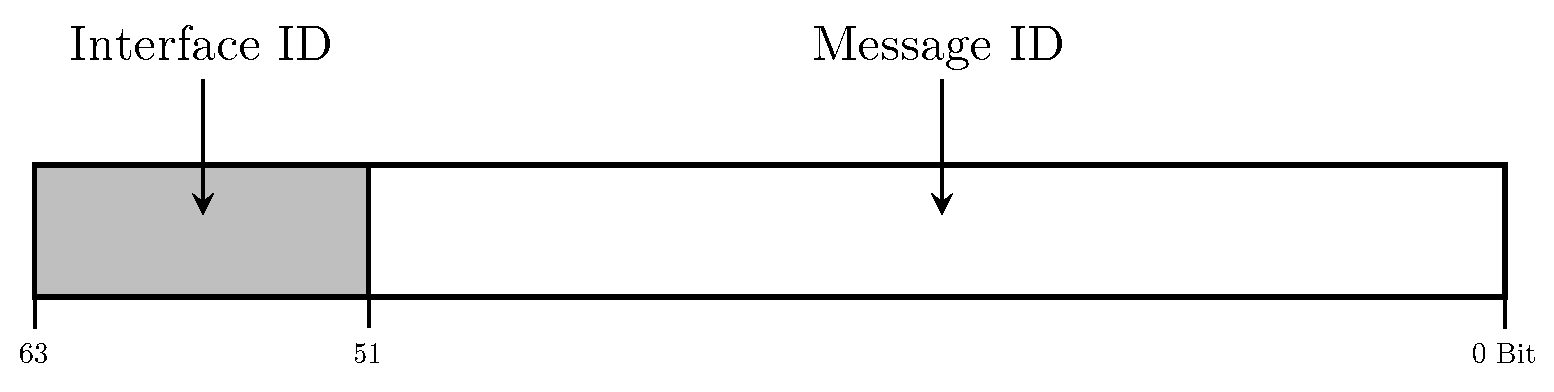
\includegraphics[width=0.8\linewidth]{figures/dml/dml01.pdf}
    \caption[Structure of the DML ID]{Structure of the DML ID. Adapted from: \cite{dml01}.}
    \label{fig:DmlId}
\end{figure}

The DML ID consists a 12-bit \textit{Interface ID} assigned to each interface by the Test Support System. In addition, a 52-bit \textit{Message ID} is part of the DML ID. This contains fields for the unique identification of a message, depending on the bus system implemented at the respective hardware interface.

The current implementation connects the involved asynchronous computer systems using a Dolphin Interconnect based on PCI Express. This connection is the focus of this thesis, since an Ethernet network based on UDP is to be investigated as a possible alternative.

Direct Memory Access (DMA) is primarily used as a method of communication between all components involved. It is described in chapter \ref{chap:hwdependcode}.

\subsection{Receive Path}

When a message is received by a hardware interface (see Figure \ref{fig:DmlRecSingleNode} and Figure \ref{fig:DmlRecMultiNode}, Arrow 1), the interface uses DMA to copy the data to a FIFO buffer (see Figure \ref{fig:DmlRecSingleNode} and Figure \ref{fig:DmlRecMultiNode}, Arrow 2). A FIFO buffer is implemented as a ring buffer and is located in the main memory of the node. Each interface has a separate FIFO buffer, which allows for asynchronous access without mutual exclusion, as the FIFO buffer is only written to by the respective interface.

The Data Manager, a process running on each node, polls all of the FIFO buffers of the node at a specified time interval. If a new message is found in a FIFO and there is a subscriber for that message, it is processed further.

If a subscriber exists on the local node, referred to as Single Node Mode, the Data Manager copies the message to the monitor memory (see Figure \ref{fig:DmlRecSingleNode}, Arrow 3). From there, it can be read by a Processing Unit.

If a subscriber for a message exists on another node, referred to as Multi Node Mode, the message must be forwarded. To achieve this, the nodes exchange subscriber lists. This forwarding process is illustrated in Figure \label{fig:DmlRecMultiNode}, Arrow 3. The Data Manager of the local node copies the message by DMA over the Dolphin Interconnect into a FIFO buffer of the remote node. Each node has, in addition to the FIFO buffers for each interface in the node, a FIFO buffer for each remote node in the distributed Test Support System.

The Data Manager of the remote node then copies the message to the monitor memory (see Figure \label{fig:DmlRecMultiNode}, Arrow 4), similar to the local distribution.

\subsection{Transmit Path}

Whenever a processing unit wants to send a message on a bus system using a hardware interface, it writes it into a FIFO buffer (see Figure \ref{fig:DmlTransSingleNode} and Figure \ref{fig:DmlTransMultiNode}, Arrow 1). These FIFO buffers are separate from the ones on the receiving side. Each node has a FIFO for every processing unit and for every other remote node in the distributed Test Support System.

The Data Manager also polls these FIFO buffers. To forward a message, it is distinguished whether the interface is located on the same node or on a remote node.

If the message is intended for an interface on the same node, referred to as Single Node Mode, the Data Manager copies it into the Transmit FIFO (Tx FIFO) of that interface (see Figure \label{fig:DmlTransSingleNode}, Arrow 2). The interface then copies the message that will be sent out next on the bus system into the Tx buffer. A composer mechanism is used to reuse certain parts of a previous message, which allows a Processing Unit to send only the parts that have changed from the prior message. The composer then builds the complete message based on this information. It is then transmitted through the front end of interface in accordance with the timing of the corresponding bus system.

If the message is intended for an interface of a remote node, the Data Manager of the local node copies it using DMA over the Dolphin Interconnect to its FIFO buffer on the remote node (see Figure \label{fig:DmlTransMultiNode}, Arrow 2). The Data Manager of the remote node then places it in the Tx FIFO of the corresponding interface (see Figure \label{fig:DmlTransMultiNode}, Arrow 3), from where it is processed and finally sent as described above.

\clearpage

\begin{figure}[!htbp]
    \centering
    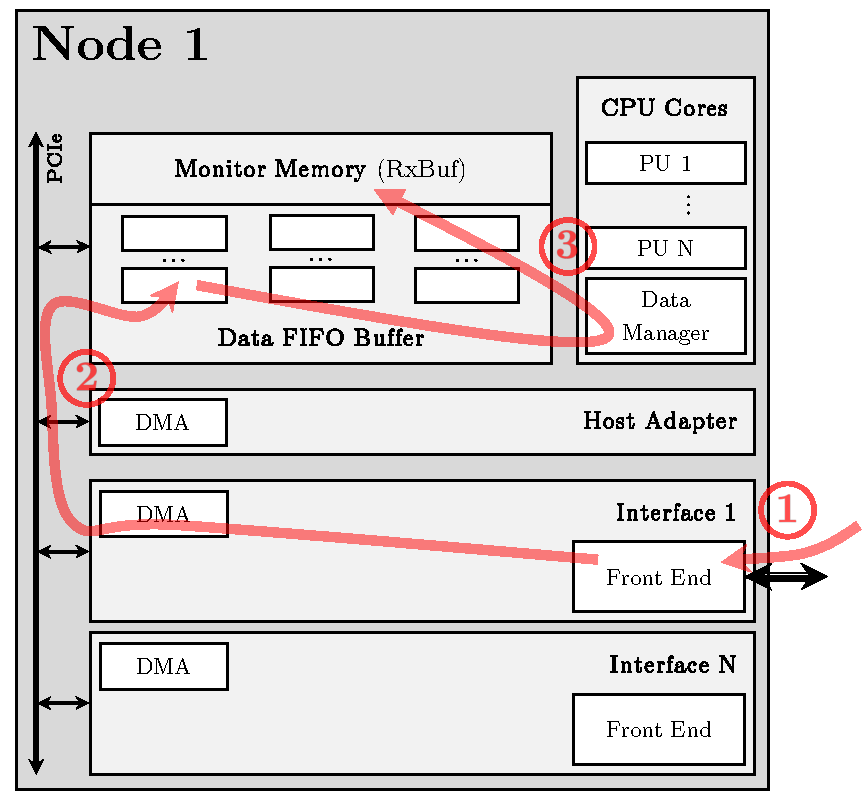
\includegraphics[width=0.58\linewidth]{figures/dml/dml02a.pdf}
    \caption[DML Receive Path in Single Node Mode]{DML Receive Path in Single Node Mode. Adapted from: \cite{dml01}.}
    \label{fig:DmlRecSingleNode}
\end{figure}

\vspace{20pt}

\begin{figure}[!htbp]
    \centering
    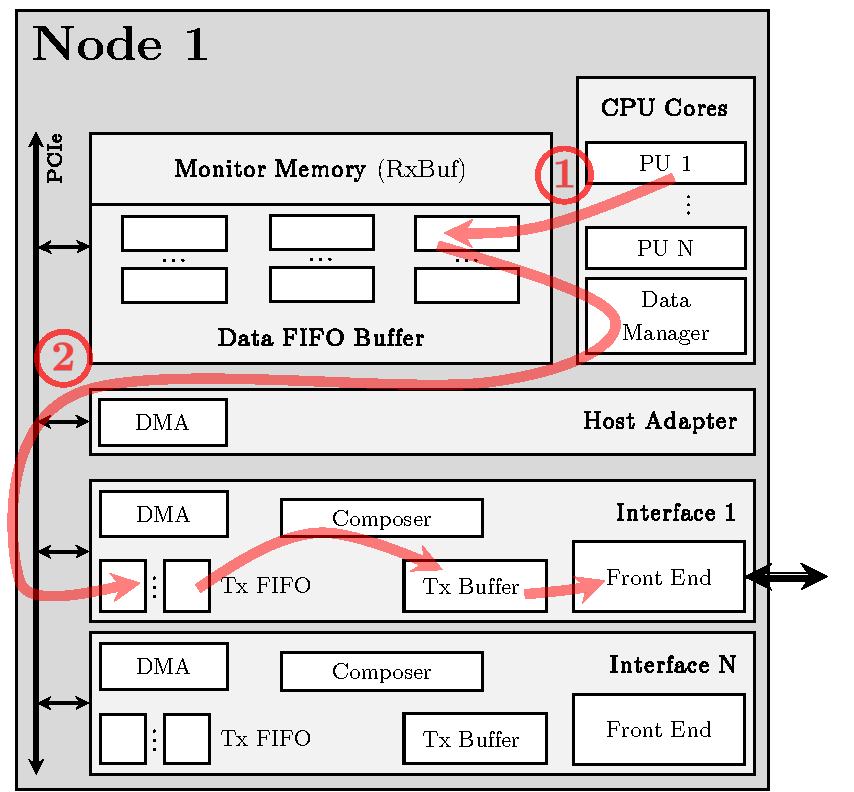
\includegraphics[width=0.58\linewidth]{figures/dml/dml03a.pdf}
    \caption[DML Transmit Path in Single Node Mode]{DML Transmit Path in Single Node Mode. Adapted from: \cite{dml01}.}
    \label{fig:DmlTransSingleNode}
\end{figure}

\begin{sidewaysfigure}[h!]
    \centering
    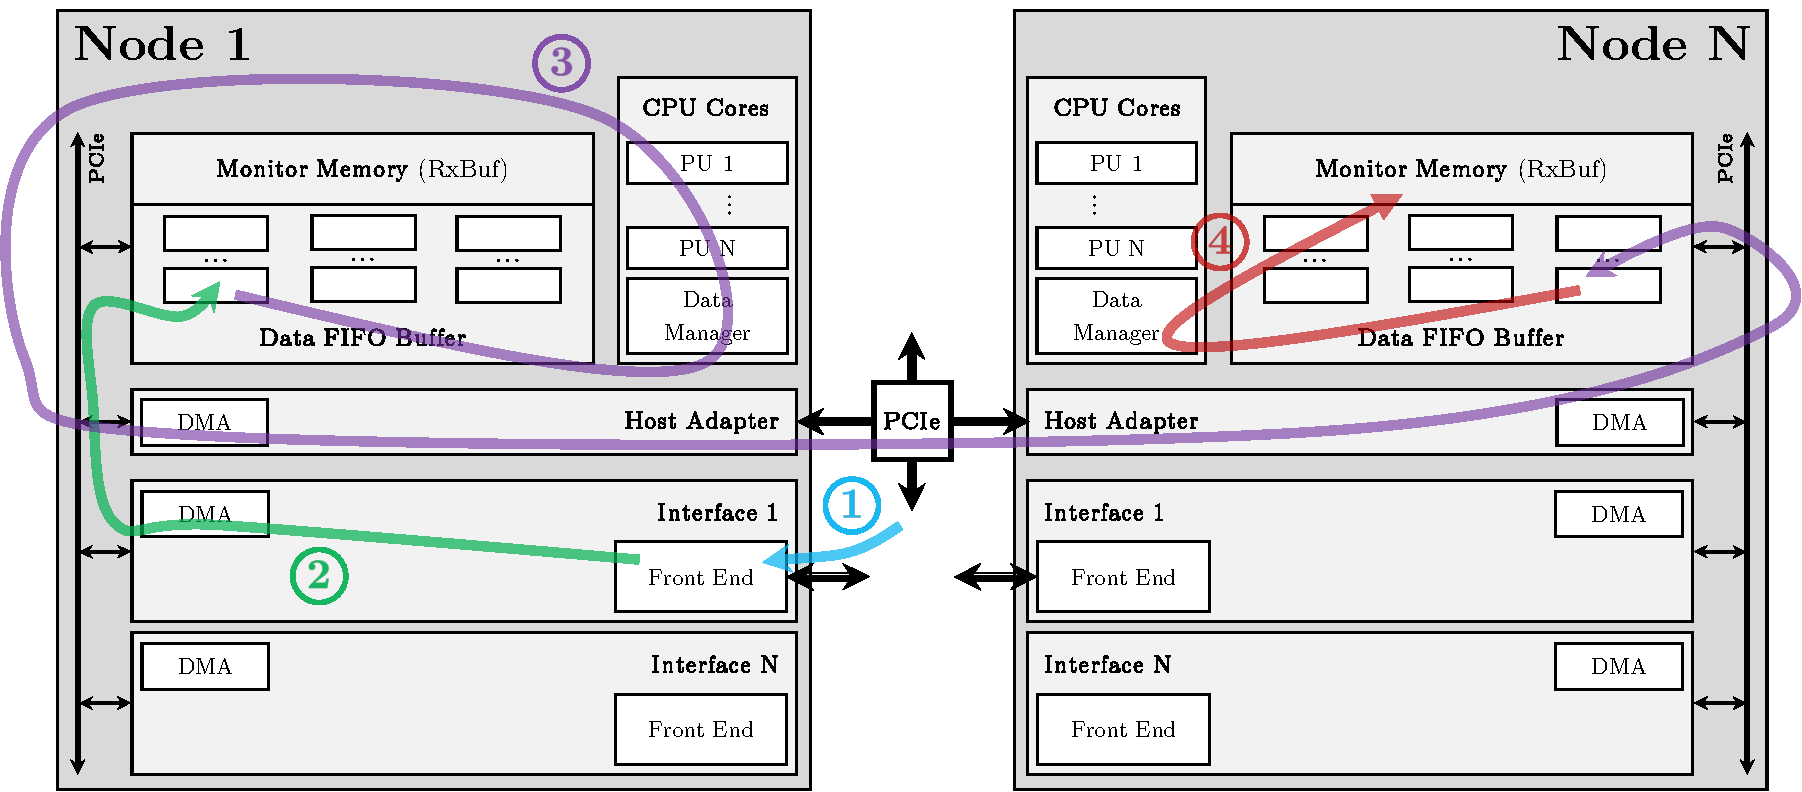
\includegraphics[width=1\linewidth]{figures/dml/dml02b.pdf}
    \caption[DML Receive Path in Multi Node Mode]{DML Receive Path in Multi Node Mode. Adapted from: \cite{dml01}.}
    \label{fig:DmlRecMultiNode}
\end{sidewaysfigure}

\begin{sidewaysfigure}[h!]
    \centering
    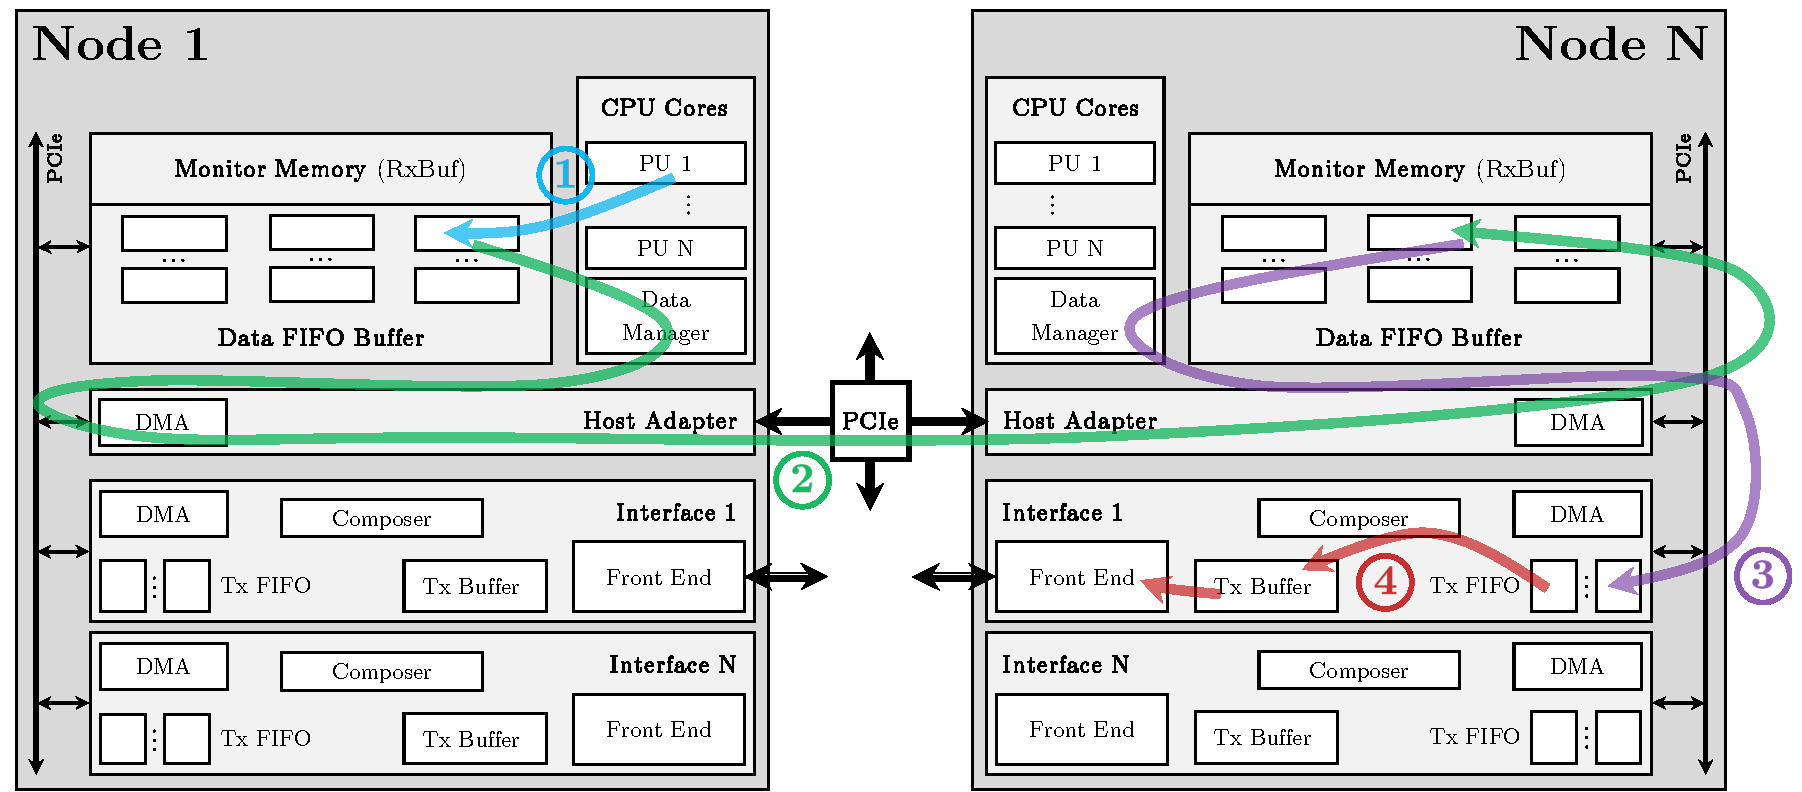
\includegraphics[width=1\linewidth]{figures/dml/dml03b.pdf}
    \caption[DML Transmit Path in Multi Node Mode]{DML Tranismit Path in Multi Node Mode. Adapted from: \cite{dml01}.}
    \label{fig:DmlTransMultiNode}
\end{sidewaysfigure}

\clearpage


\section{TCP/IP Reference Model} \label{chap:RefModel}

Protocols are the basis for communication between instances in a network. They specify rules that must be followed by all communication partners \cite{Tanenbaum2010}. Reference models arrange protocols hierarchically in layers. Each layer solves a specific part of the communication task and uses the services of the layer below while providing certain services to the layer above \cite{Weigel2021}.

\begin{figure}[h]
    \centering
    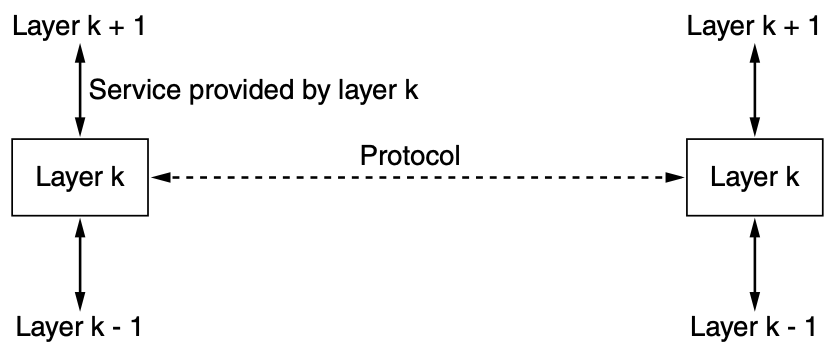
\includegraphics[width=0.7\linewidth]{figures/tcpip_refmodel/image1.png}
    \caption[Relationship between service and protocol]{Relationship between service and protocol. Source: \cite{Tanenbaum2010}.}
    \label{fig:ServiceProtRelation}
\end{figure}

Figure \ref{fig:ServiceProtRelation} illustrates the relationship between service and protocol. A service refers to a set of operations that a layer provides to the layer above it, and it defines the interface between the two layers \cite{Tanenbaum2010}.

A protocol is a set of rules that define the format of messages exchanged within a layer \cite{Tanenbaum2010}. These rules define the implementation of the service offered by the layer The transparency principle applies, meaning that the implementing protocol is transparent to the service user and can be changed as long as the service offered remains unchanged \cite{Weigel2021}.

\begin{figure}[h!]
    \centering
    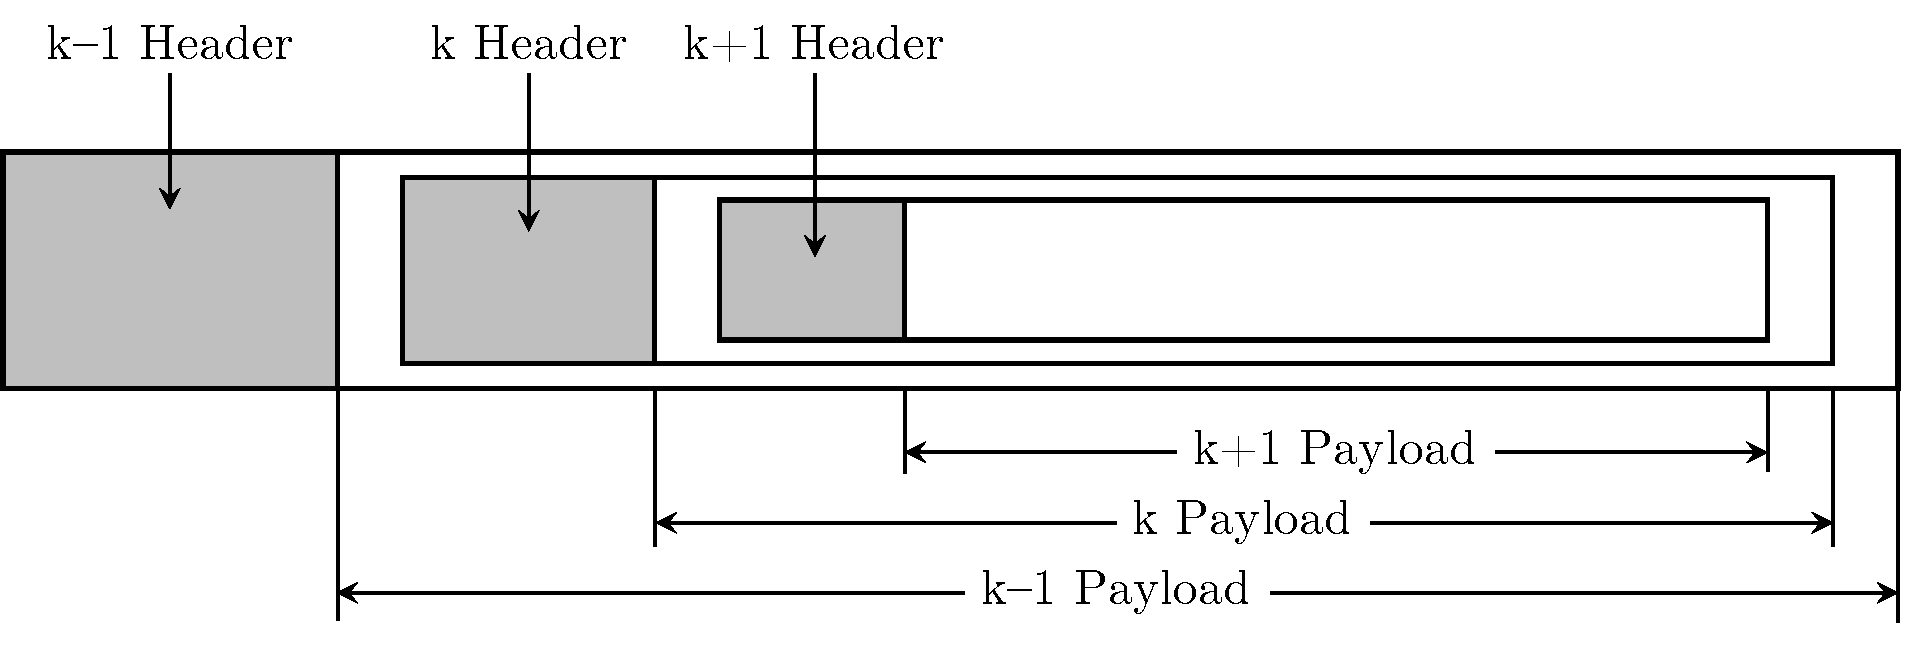
\includegraphics[width=1\linewidth]{figures/tcpip_refmodel/image2.pdf}
    \caption[Encapsulation Principle]{Encapsulation Principle. Adapted from: \cite{Tanenbaum2010}.}
    \label{fig:EncapsulationPrinciple}
\end{figure}

Protocols define the format of control information required by layer k to provide the service. This information is attached as a header or trailer to the data of layer k + 1, known as the payload, and is removed by the receiving instance. This principle is known as the 'Encapsulation Principle' and is illustrated in Figure \ref{fig:EncapsulationPrinciple} \cite{Tanenbaum2010}.



\subsection{Introduction of the Reference Model}

The following section presents a explanation of the TCP/IP reference model. Throughout this section, we will refer to the hybrid reference model proposed by Andrew S. Tanenbaum in \cite{Tanenbaum2010}. Figure \ref{fig:RefModel} shows this hybrid reference model. The physical layer is at the bottom, and the application layer is at the top. The tasks of each layer are briefly described here. For additional information, please refer to \cite{Tanenbaum2010}.

\begin{figure}[h]
    \centering
    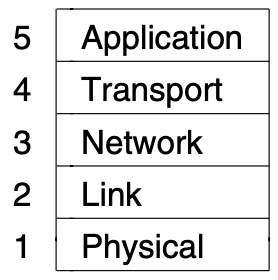
\includegraphics[width=0.25\linewidth]{figures/tcpip_refmodel/image3.png}
    \caption[Hybrid TCP/IP Reference Model]{Hybrid TCP/IP Reference Model. Source: \cite{Tanenbaum2010}.}
    \label{fig:RefModel}
\end{figure}
	
	
\begin{itemize}
\item The \textbf{Physical Layer} serves as the interface between a network node and the transmission medium, responsible for transmitting a bit stream. This involves line coding, which converts binary data into a signal. Additionally, the physical layer encompasses the transmission medium and the connection to this medium \cite{Tanenbaum2010, Weigel2021}.
\item The \textbf{Link Layer} facilitates reliable transmission of a sequence of bits (called a frame) between adjacent network nodes. This encompasses frame synchronization, which involves detecting frame boundaries in the bit stream, error protection, flow control, channel access control, and addressing \cite{Weigel2021}.
\item The \textbf{Network Layer} provides end-to-end communication between two network nodes. This includes addressing and routing \cite{Tanenbaum2010, Weigel2021}.
\item The \textbf{Transport Layer} provides the transfer of a data stream of any length between two application processes. This involves collecting outgoing messages from all application processes and distributing incoming messages to them \cite{Weigel2021}.
\item The \textbf{Application Layer} serves as the interface to the application. It is responsible for implementing protocols for network use, such as file transfer or network management \cite{Weigel2021}.
\end{itemize}



\subsection{Protocols of the Reference Model} \label{chap:ProtosRefModel}

\begin{figure}[h]
    \centering
    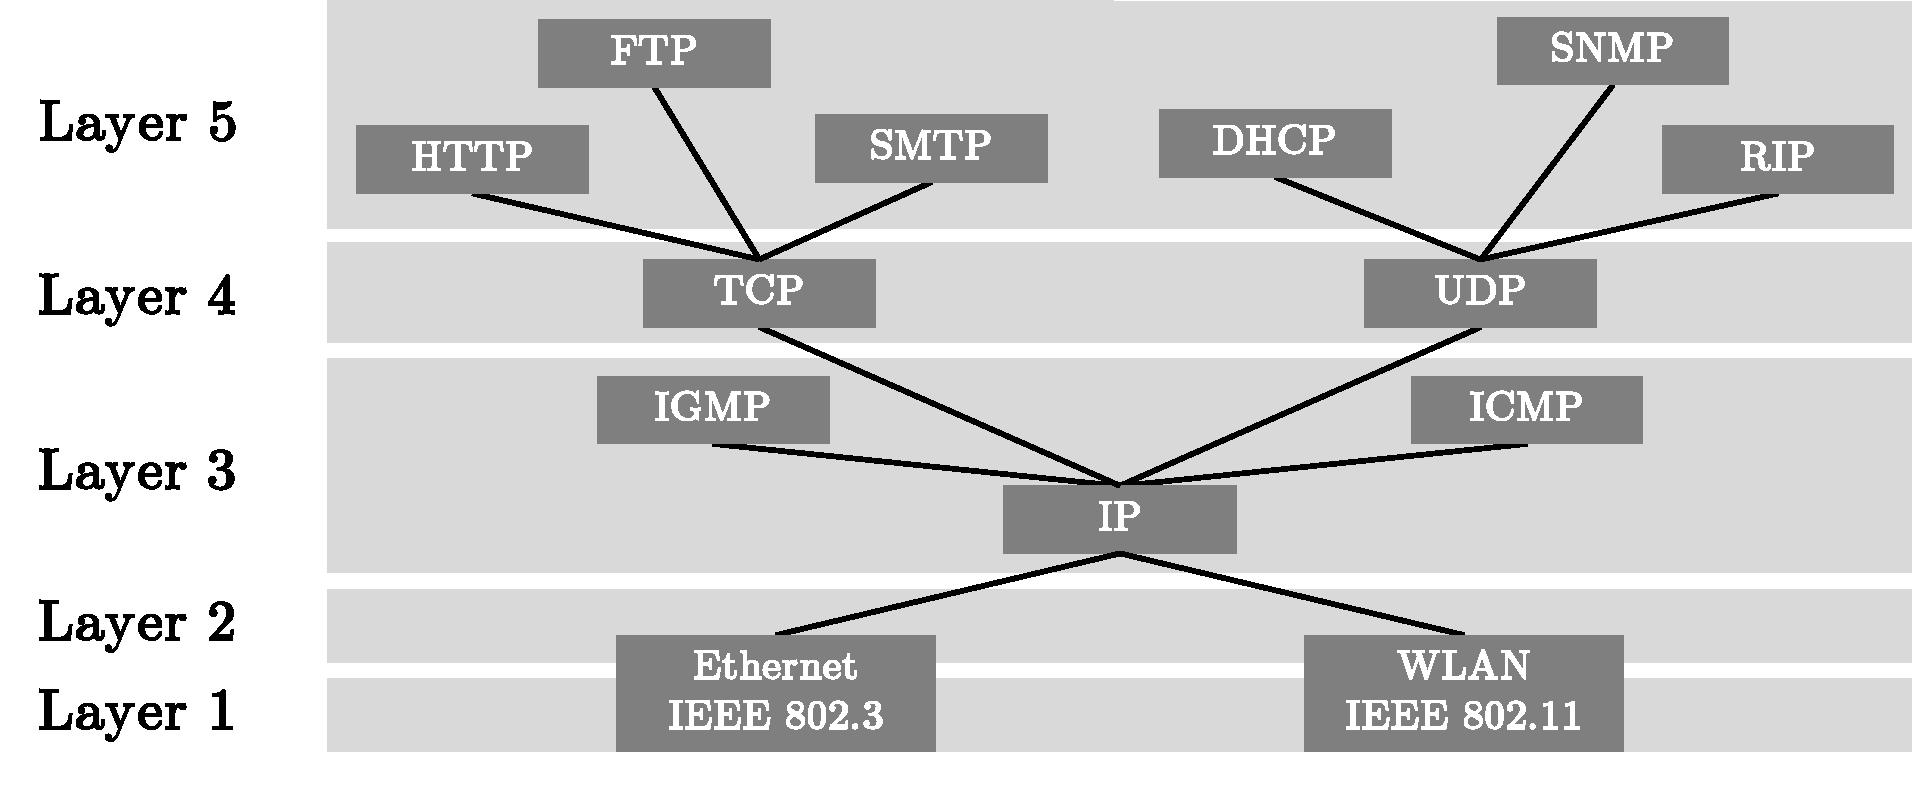
\includegraphics[width=1\linewidth]{figures/tcpip_refmodel/image4.pdf}
    \caption[Selection of important protocols of the hybrid TCP/IP Reference Model]{Selection of important protocols of the hybrid TCP/IP Reference Model. Adapted from: \cite{Weigel2021}.}
    \label{fig:RefModelProtos}
\end{figure}

Figure \ref{fig:RefModelProtos} shows a selection of important protocols of the TCP/IP reference model including their assignment to the respective layer. The illustration also shows the dependency of the protocols on each other.

In this section, the characteristics of the protocols TCP, UDP, IP and Ethernet (IEEE 802.3), which are relevant for this work, are explained in detail according to \cite{Tanenbaum2010}. Further information about the protocols of the TCP/IP reference model can be found in \cite{Tanenbaum2010}.


\subsubsection{Ethernet (IEEE 802.3)}
Ethernet, as defined by IEEE standard 802.3, specifies both hardware and software for wired data networks.  This means that Ethernet includes both the physical layer and the link layer of the presented hybrid TCP/IP reference model.


\paragraph{Ethernet Physical Layer}
The Ethernet physical layer consists of a number of standards that define different media types associated with different transmission rates and cable lengths. 

Ethernet defines physical layer standards with transmission rates ranging from 10 Mbit/s to 1.6 Tbit/s, which is currently under development as the 802.3dj standard \cite{IEEEOpeningPlenary}. Both fiber and copper are used as transmission media. In the following, the 802.3an standard will be briefly discussed, since it is the one that will be used most in this thesis.

The 802.3an standard was published in 2006 and defines data transmission with a transmission rate of 10 Gbit/s over twisted-pair cables \cite{10GigabitEthernet}, also referred to as 10 GbE. Twisted-pair cables are copper cables in which pairs of copper wires are twisted together to reduce electromagnetic interference. Twisted-pair cables are divided into categories based on various characteristics, such as shielding or twist strength \cite{isoiec11801}. For 802.3an, a maximum cable length of 100 meters is specified in conjunction with Cat7 cables. 802.3an specifies the RJ45 connector as the plug connector.

According to 802.3an, the PAM16 line coding is used for Ethernet at 10 Gbps. It uses the principle of pulse amplitude modulation, which is described in detail in \cite{PulseAmplitudeModulation}. PAM16 allows the transmission of data by varying the amplitude of a signal in 16 different stages. Each stage represents four bits of information.

In addition to 802.3an, the Ethernet physical layer according to 802.3ae was also used in this work. This also defines the physical layer with a transmission rate of 10 Gbit/s. However, fiber optic cables are used in conjunction with transceiver modules called SPF+ SR \cite{10GigabitEthernet}.

\paragraph{Ethernet Link Layer} \label{chap:EthLinkLayer}
At the link layer, Ethernet defines frame formatting, addressing, error detection, and access control. This is also called the Medium Access Control (MAC) sublayer.

\begin{figure}[h]
    \centering
    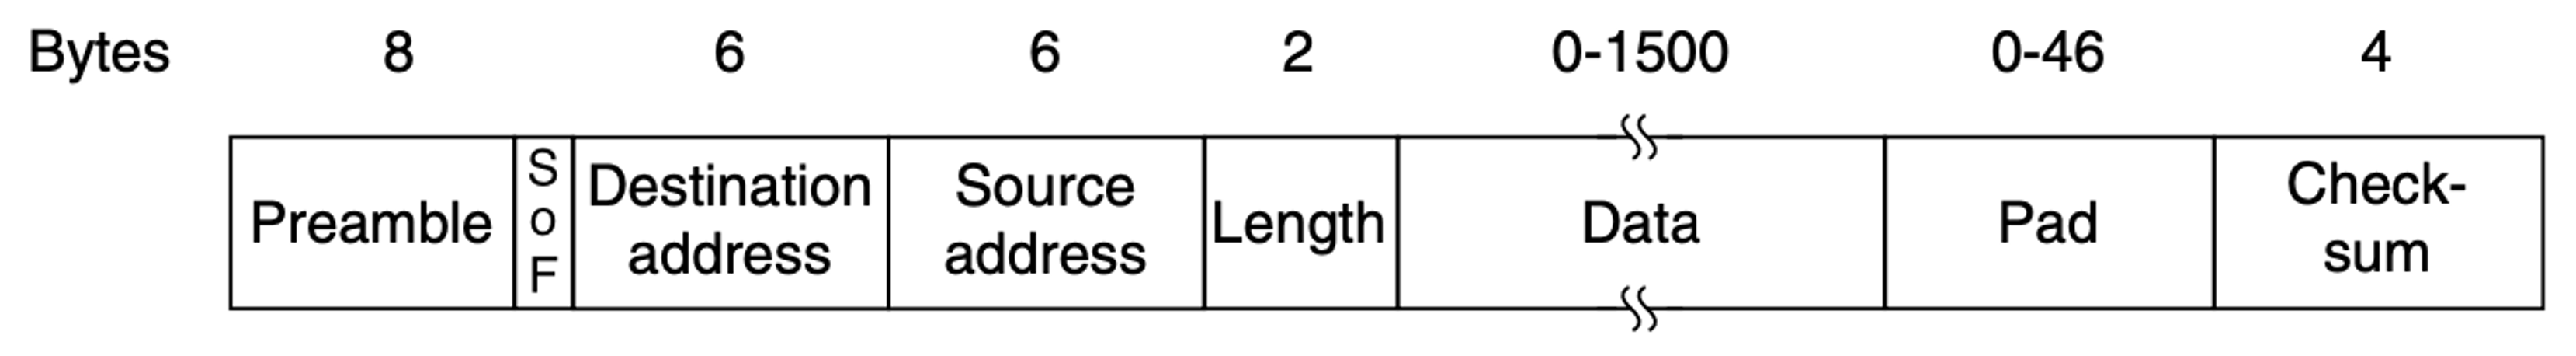
\includegraphics[width=1\linewidth]{figures/tcpip_refmodel/image5.png}
    \caption[Structure of the Ethernet frame]{Structure of the Ethernet frame. Source: \cite{Tanenbaum2010}.}
    \label{fig:EthernetFrame}
\end{figure}

Figure \ref{fig:EthernetFrame} shows the IEE 802.3 frame format. The Ethernet header consists of the fields '\textit{Destination address}', '\textit{Source address}' and '\textit{Length}' and therefore has a size of 14 bytes.

Each frame begins with a \textit{preamble}. This has a length of 8 bytes and contains the bit sequence 10101010. An exception is the last byte, which contains the bit sequence 10101011 and is referred to as the \textit{Start of Frame} (SoF). The preamble is used for synchronization between the sender and receiver. The last byte of the preamble marks the start of a frame \cite{Tanenbaum2010}.

This is followed by the \textit{destination} and \textit{source address}. This is the MAC address, which is uniquely assigned globally to a network interface \cite{Weigel2021}. This consists of a manufacturer code with a length of 3 bytes, followed by the serial number of the network interface, which also has a length of 3 bytes. The MAC address enables the Ethernet protocol to uniquely identify a station in the local network.

The \textit{Length} field specifies the length of the data field. In IEEE 802.3 Ethernet, this has a maximum length, called the Maximum Transfer Unit (MTU), of 1500 bytes. However, there are Ethernet implementations that use a larger MTU than specified in the original standard. These are known as jumbo frames \cite{EthernetJumboFrames2009}. Jumbo frames can increase network throughput and reduce CPU usage, as demonstrated in studies \cite{swsetup03}. It is important to ensure that all network participants support jumbo frames to avoid packet loss \cite{swsetup04}.

In addition to a maximum length, the Ethernet standard also specifies a minimum length. An entire Ethernet frame must therefore have a minimum length of 64 bytes from the destination address to the checksum. To ensure that this can be achieved even with a small data field, padding information is added. The specification of the minimum length is related to the access control used.

The Ethernet frame ends with a 4-byte \textit{checksum} that is used for the Cyclic Redundancy Check (CRC) based on polynomial divisions, as explained in \cite{Tanenbaum2010}.  This checksum serves to detect errors during transmission.

Ethernet originally used a shared transmission medium, allowing multiple communication participants to use it simultaneously. To control access, the MAC sublayer employs the CSMA/CD algorithm, ensuring that only one device transmits data at a time. Each device listens to the medium (carrier sense) before sending data to determine whether it is free. It also performs collision detection to determine whether two devices have started sending at the same time. In such a case, the devices stop the transmission and retry it after a random waiting time to avoid the collision \cite{Tanenbaum2010}.

The 802.3an specification for 10 Gigabit Ethernet is exclusively for point-to-point full-duplex connections, which eliminates the need for access control such as CSMA/CD. As a result, it is no longer included in the specification \cite{10GbEDefinition}.

In order to connect multiple network devices with point-to-point connections, Ethernet switches are used. They have multiple ports and forward packets based on the MAC address. Ethernet switches operate on layer 2 of the reference model.

To summarise, with Ethernet there is no guarantee that data will be transmitted reliably and without loss. Although Ethernet uses CRC for error detection, faulty frames are generally discarded. Additionally, Ethernet does not provide flow control or overload detection, which must be performed by a higher layer.


\subsubsection{IP}

The Internet Protocol (IP) is a central protocol in the TCP/IP reference model. Its tasks include connecting different networks, addressing network participants, and fragmenting packets \cite{Weigel2021}. IP is a connectionless protocol that operates on the 'best effort' principle, meaning it does not guarantee delivery.

There are two versions of the Internet Protocol: IPv4 and IPv6. As this work uses the IPv4 protocol, it is presented in more detail below.

\paragraph{IP Header} \label{chap:ipheader}

The IPv4 datagram is divided into a header and a payload. The header typically spans 20 bytes, but may also include an optional variable-length section. The header is shown in Figure \ref{fig:IPHeader}.

\begin{figure}[h]
    \centering
    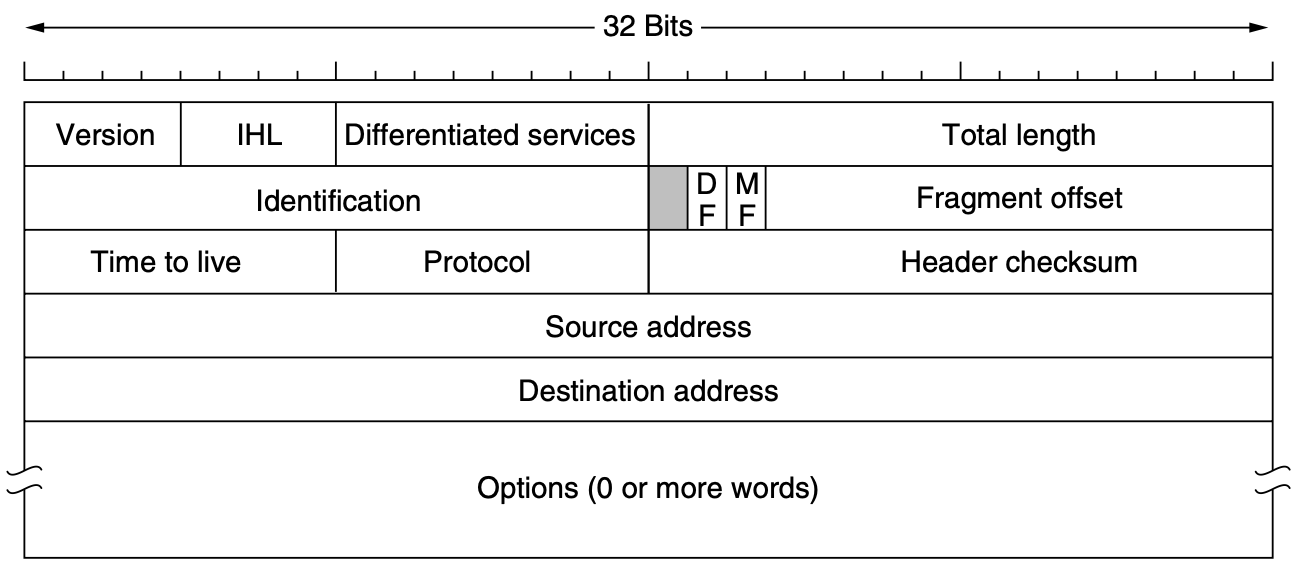
\includegraphics[width=1\linewidth]{figures/tcpip_refmodel/image7.png}
    \caption[Structure of the IP Header]{Structure of the IP Header. Source: \cite{Tanenbaum2010}.}
    \label{fig:IPHeader}
\end{figure}

The first field in the header is the 4-bit \textit{Version} field. This indicates the IP version used. For IPv4, the value is always 4.

The \textit{IHL} (Internet Header Length) field specifies the number of 32-bit words in the header. This is necessary because the header can contain options and therefore has a variable length. The minimum value of the field is 5 if there are no options.

The \textit{Differenciated Services} field specifies the service class of a packet, allowing for prioritisation of certain data traffic using Quality of Service (QoS). For a more detailed description of Quality of Service, please refer to section \ref{background:tuning:qualityofservice}.

The \textit{Total Length} field indicates the total length of the datagram, including the header. Due to the field size of 16 bits, the maximum length is 65535 bytes. However, a packet's length is also limited by the Layer 2 MTU \cite{Weigel2021}, resulting in datagrams being split into multiple packets, known as fragmentation. 

The \textit{Identification} field is assigned a number by the sender, which is shared by all fragments of a datagram.

A flag field with a length of 3 bits follows, with the first bit being unused. The second section includes the 'Don't Fragment' (\textit{DF}) flag, which indicates that intermediate stations should not fragment this packet. The third section contains the 'More Fragments' (\textit{MF}) flag, which indicates whether additional fragments follow. This flag is set for all fragments except the last one of a datagram.

The \textit{Fragment Offset} field specifies the position of a fragment in the entire datagram.

The \textit{Time to live} (TTL) field specifies the maximum lifetime of a packet. The TTL value is measured in seconds and can be set to a maximum of 255 seconds. This is done to prevent packets from endlessly circulating in the network.

The \textit{Protocol} field identifies the Layer 4 protocol used for the service. This allows the network layer to forward the packet to the corresponding protocol of the transport layer. The numbering of the protocols is standardized throughout the Internet.

The \textit{Header checksum} field contains the checksum of the fields in the IP header. The IP datagram's user data is not verified for efficiency reasons \cite{Holtkamp2024Internet}. The checksum is calculated by taking the 1's complement of the sum of all 16-bit half-words in the header. It is assumed that the checksum is zero at the start of the calculation for the purpose of this algorithm.

The two 32-bit fields \textit{Source Address} and \textit{Destination Address} contain the Internet Protocol address, called the IP address. Section \ref{chap:IPandRouting} provides further details on this topic.

The \textit{Options} field can be used to add additional information to the IP protocol. For example, there are options to mark the route of a packet.


\paragraph{IP Addresses and Routing} \label{chap:IPandRouting}

This section provides a brief description of the structure and important properties of IP addresses. The network examined in this thesis is an isolated local network that is not connected to other networks. As a result, the network layer does not perform any routing based on IP addresses. For further information on routing, please refer to \cite{Tanenbaum2010}.

\begin{figure}[h]
    \centering
    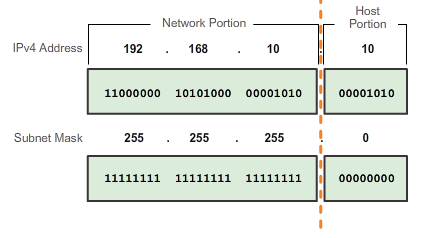
\includegraphics[width=0.8\linewidth]{figures/tcpip_refmodel/image8.png}
    \caption[Structure of the IP address and subnet mask]{Structure of the IP address and subnet mask. Source: \cite{CSE252ImageSubnet}.}
    \label{fig:IPSubnet}
\end{figure}

Every participant on the Internet has a unique address, known as an IP address. This has a total length of 32 bits and a hierarchical structure that divides the IP address into a network portion and a host portion. The division between the two parts is variable and is defined by a so-called subnet mask, which is illustrated in Figure \ref{fig:IPSubnet}. The bits of the network portion of the IP address are marked with ones.

\begin{itemize}
\item The \textbf{network portion} identifies a specific network, such as a local Ethernet network, and is the same for all participants in this network.
\item The \textbf{host portion} identifies a specific device within this network.
\end{itemize}

Routing, which is another important task of the network layer, is based on IP addresses. The packet can be directed to its destination using the network portion of the IP address. The path to the destination is determined by specific routing algorithms. As mentioned earlier, the thesis only considers an isolated local network, so further discussion on routing will be omitted.


\paragraph{Address Resolution Protocol}

The Address Resolution Protocol, abbreviated to ARP, is an auxiliary protocol of the network layer. Its task is to map the IP addresses to a MAC address and vice versa, as the sending and receiving of data in the underlying link layer is based on these MAC addresses \cite{Weigel2021}.


\paragraph{Fragmentation and Defragmentation} \label{chap:frag}

As explained in \ref{chap:EthLinkLayer}, the link layer defines a maximum data size known as MTU. Since IPv4 datagrams have a maximum size of 65535 bytes, they must be divided into smaller packets, or fragments, each with its own IP header.

The IP header (refer to Figure \ref{fig:IPHeader}) contains information necessary for the target system to assemble fragmented packets, a process known as defragmentation. This includes the ID that assigns all fragmented packets to a datagram, as well as the fragment offset that specifies their position within the datagram. The 'More Fragment' flag indicates whether additional fragments will follow.

Fragmentation has the advantage of allowing IPv4 datagrams larger than the MTU to be sent, but the disadvantage is that the loss of a single fragment results in the loss of the entire datagram. Additionally, fragmentation can cause packet reordering \cite{IPFragDetail}.

\subsubsection{TCP and UDP}
TPC and UDP are transport layer protocols. As a service, they provide the transmission of a data stream of any length between two application processes. The services of the network layer are used for this purpose.

\paragraph{TCP}

TCP provides \textbf{reliable} transmission of a byte stream in a \textbf{connection-oriented} manner. A virtual connection is established between the two instances before transmission, which is terminated after transmission.

TCP also implements flow control to ensure reliable data transfer between sender and receiver without losses and to prevent overloading at the receiver.  TCP provides congestion control to prevent network overload and ensures reliable transmission using Positive Acknowledgement with Re-Transmission (PAR) algorithm \cite{Holtkamp2024Transport}.  

TCP is known for its secure data transmission. However, it requires a significant amount of control information to implement its functions. The Transmission Control Protocol (TCP) header is 20 bytes in size. In addition to an application identifier (port number), it contains flow control and congestion control information. This overhead can negatively impact transmission speed. Additionally, the data loss from the underlying layers combined with the flow control used by TCP leads to delays and reduced throughput, which can have a significant impact on the performance of the application.

\paragraph{UDP}

In contrast to TCP, UDP is an \textbf{unreliable} and \textbf{connectionless} protocol. The protocol sends packets, called datagrams or segments, individually. UDP lacks mechanisms for detecting the loss of individual datagrams, and the correct sequence of these is not guaranteed.

\begin{figure}[h]
    \centering
    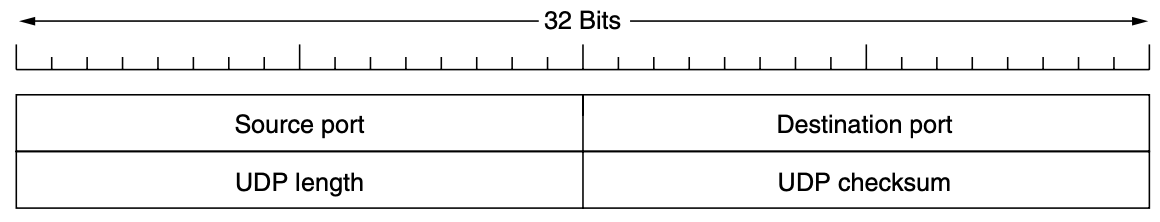
\includegraphics[width=1\linewidth]{figures/tcpip_refmodel/image6.png}
    \caption[Structure of the UDP Header]{Structure of the UDP Header. Source: \cite{Tanenbaum2010}.}
    \label{fig:UDPHeader}
\end{figure}

Figure \ref{fig:UDPHeader} displays the UDP header, which has a size of 8 bytes. It is considerably smaller than the TPC header, which has a size of 20 bytes.

The header includes the fields \textit{Source port} and \textit{Destination port} to identify the endpoints in the respective instance. When a packet arrives, the payload is passed to the application using the appropriate port number via the UDP protocol.

The \textit{UDP length} field indicates the length of the segment, including the header. The maximum length of data that can be transmitted via UDP is limited to 65,515 bytes due to the underlying Internet Protocol.

The last field of the header is a 16-bit \textit{UDP checksum}. This checksum is formed via the so-called IP pseudoheader, which contains the source and destination IP address, the protocol number from the IP header, and the \textit{UDP length} field of the UDP header.

Compared to TCP, UDP can achieve higher data transmission speeds due to its lower protocol overhead, ase the UDP header is only 8 bytes in size. Furthermore, UDP does not require an acknowledgement of the transport or other mechanisms used by TCP to provide a reliable connection. This makes it very efficient and reduces processing overhead.








\section{Linux Kernel}

The Linux kernel is an operating system kernel that is available under a free software license and has been under development since 1991 \cite{like01}. The Linux kernel is the main component of a Linux operating system and is used by a large number of operating systems, called distributions. Popular examples of such distributions are Ubuntu or Linux Mint, which are used in this thesis.

This chapter will take a closer look at the Linux kernel. However, due to the scope of the Linux kernel, readers are referred to \cite{like02}, \cite{like03} and \cite{like08}, which provide a detailed and comprehensible insight into the Linux kernel. Additionally, a basic knowledge of operating systems is required, which can be obtained from \cite{like05}.

An operating system kernel serves as the interface between the hardware and the processes of a computer system \cite{like04}. It manages hardware resources, schedules processes, and facilitates communication between application software and hardware \cite{like06}.

\begin{figure}[h]
    \centering
    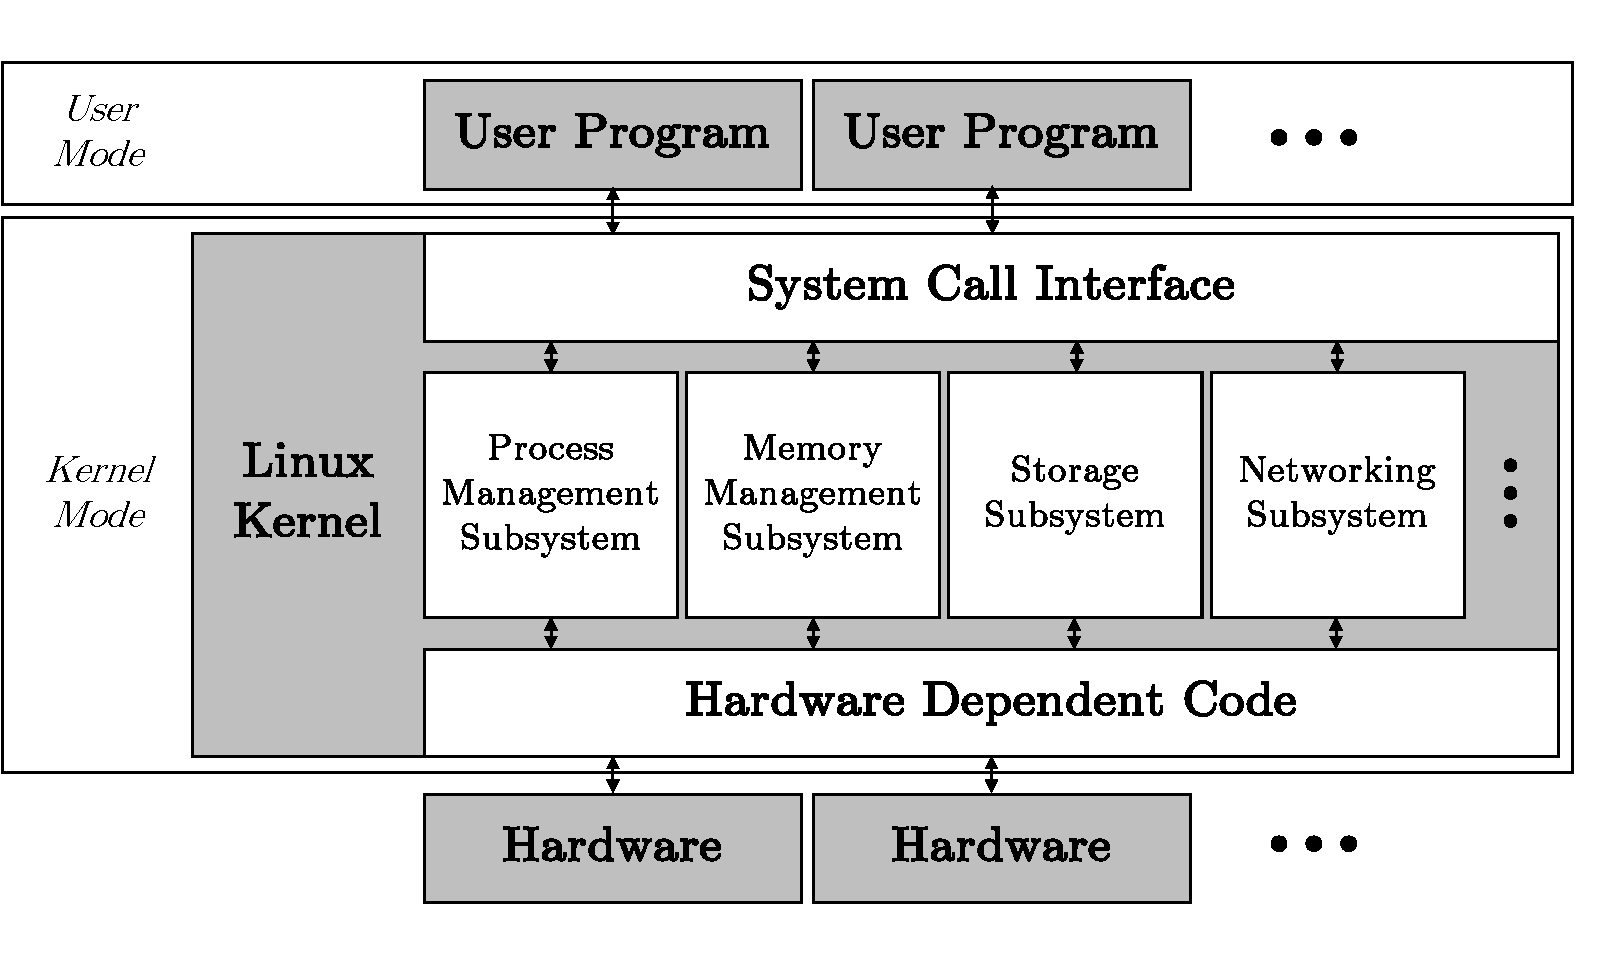
\includegraphics[width=1\linewidth]{figures/linux_kernel/image01.pdf}
    \caption[Simplified representation of the Linux Kernel with selected Subsystems]{Simplified representation of the Linux Kernel with selected Subsystems.}
    \label{fig:LinuxKernel}
\end{figure}

Figure \ref{fig:LinuxKernel} presents a condensed overview of the architecture of a Linux operating system. The illustration highlights some selected features of the kernel.

Linux consists of a monolithic kernel. This means that the entire kernel is implemented as a single program, and all kernel services run in a single address space. Communication within the kernel is achieved through function calls \cite{like02}.

This is in contrast to the microkernel, which divides functionalities into separate modules and uses message passing for communication between them. Although the Linux kernel is based on a monolithic approach, it adopts some aspects of a microkernel, such as a modular architecture with different subsystems or the ability to load modules dynamically. However, communication within the kernel occurs through function calls, which provides better performance compared to message passing \cite{like08}.

In the following, the characteristics of the Linux kernel and its environment shown in Figure \ref{fig:LinuxKernel} are described.


\subsection{User Mode and Kernel Mode}

The Linux architecture distinguishes between two basic execution environments: user mode and kernel mode. Application processes run in user mode with restricted rights, while the Linux kernel, which is the main part of the operating system, runs in kernel mode \cite{like02}.

This separation requires corresponding support in the processor. This system monitors aspects such as memory access, branches, or the executed instruction set in user mode and intervenes in the event of unauthorized access, for example, by stopping the process \cite{like06}. The transition between the different execution environments occurs as part of a system call.


\subsection{System Call Interface}

Processes that request a service from the Linux kernel use system calls. These calls are made through a software interrupt (trap), which causes the CPU to switch to kernel mode and call the so-called system call handler. In the handler, the requested service is identified using an ID transmitted by the user process, and the corresponding instructions are invoked \cite{like02}. A process or application executes a system call in kernel space. This is also referred to as the kernel running in the context of the process.

In the monolithic kernel, individual instructions call other instructions of the kernel.  This sequence of instructions, executed during a system call, is referred to as the \textit{kernel control path} \cite{like07}.

The Linux kernel is a \textit{reentrant kernel}. Several processes can be executed simultaneously in kernel mode, which also means that the process can be interrupted while instructions are being executed in kernel mode. Functions in a reentrant kernel should therefore only change local variables and not affect global data structures. However, there are also non-reentrant functions in the kernel, for which corresponding locking mechanisms are used \cite{like02}.

It should be noted here that system calls are not the only way to execute instructions in the kernel. According to \cite{like02}, there exist other ways besides system calls:

\begin{itemize}
\item A exception is reported by the CPU, which are handled by the kernel for the originating process. An example of this is the execution of an invalid instruction.
\item A peripheral device sends an interrupt signal to the CPU, which is processed by a function called the interrupt handler. As peripheral devices work asynchronously to the CPU, interrupts occur at unpredictable times.
\item A kernel thread is executed. These run in kernel mode and are mainly used to perform certain tasks periodically.
\end{itemize}


\subsection{Hardware and Hardware Dependent Code} \label{chap:hwdependcode}

As already mentioned, the kernel is the interface between the hardware and the processes of a system. Many operations in the kernel are related to the access of physical hardware.

The Linux kernel distinguishes between three different types of hardware devices [8]:

\begin{itemize}
\item \textbf{Block Devices} – devices with block-oriented addressable data storage (e.g. hard drives)
\item \textbf{Character Devices} – devices that handle data as a stream of characters or bytes (e.g. keyboards)
\item \textbf{Network Devices} – devices that provide access to a network
\end{itemize}

The abstraction layer between the physical hardware and the Linux kernel are device drivers. Their primary function is to initialize the device and register its capabilities with the kernel. Additionally, drivers enable the kernel to access, control, and communicate with the device. Each driver is specific to a device and implements certain predefined interface functions to the Linux kernel, depending on the type of the device. The device drivers are available as modules that can be loaded dynamically at runtime \cite{like09}.

One way for the physical hardware to interact with the kernel via the device drivers is through interrupts, which is referred to as \textit{Interrupt-Driven I/O}. The hardware uses \textit{interrupt requests} to inform about certain events, and the driver implements the associated \textit{interrupt handler} to process the request \cite{like09}.

\textit{Direct Memory Access} (DMA) is another way of interaction between the hardware and a system, which is mainly used by block devices or network devices [9]. DMA is a mechanism that allows hardware devices to transfer data directly to or from system memory, bypassing the CPU. This method enhances data throughput and system performance, as it reduces CPU overhead during high-volume data transfers \cite{like05}.

Additional information regarding the interface between the Linux kernel and hardware, as well as device drivers, can be found in \cite{like09}.


\subsection{Kernel Subsystems}

As previously stated, the Linux kernel is a monolithic kernel that is subdivided into various subsystems. A subsystem is a group of functions that work together to perform a specific task. Figure \ref{fig:LinuxKernel} displays the most significant subsystems, which are further explained below based on \cite{like03} and \cite{like09}.

\subsubsection{Process Management Subsystem}
The process management subsystem is responsible for the administration of processes. This task can be divided into three main parts:

\begin{itemize}
\item Creation and termination of processes and their related resources
\item Communication between different processes (e.g. with \textit{Signals} or \textit{Pipes})
\item Scheduling
\end{itemize}

\subsubsection{Memory Management Subsystem}
The primary function of the memory management subsystem is \textit{Virtual Memory Management}. This enables more efficient use of RAM. Each process is assigned a virtual address space, and parts of it that are not currently required can be swapped to disk. This is based on the locality principle of programs. Additionally, \textit{Virtual Memory Management} enables isolation between processes.

The memory management subsystem in the Linux kernel provides memory for other kernel modules, for example through malloc/free operations.

\subsubsection{Storage Subsystem}
The storage subsystem is responsible for creating and managing the file system on the physical media, such as the disk.


\subsubsection{Networking Subsystem}
The networking subsystem handles the sending and receiving of packets in networks and their distribution to applications in user space. Additionally, it implements network protocols such as those used by the TCP/IP protocol stack presented in \ref{chap:ProtosRefModel}.

A detailed description of specific parts of the networking subsystem can be found in chapter \ref{chap:LinuxUDPNWStack}.







\section{UDP communication with a Linux Operating System} \label{chap:LinuxUDPNWStack}
The purpose of this chapter is to explain UDP communication using a Linux operating system. The fundamental processes are described, with an emphasis on the interaction among the different components.

\begin{figure}[h]
    \centering
    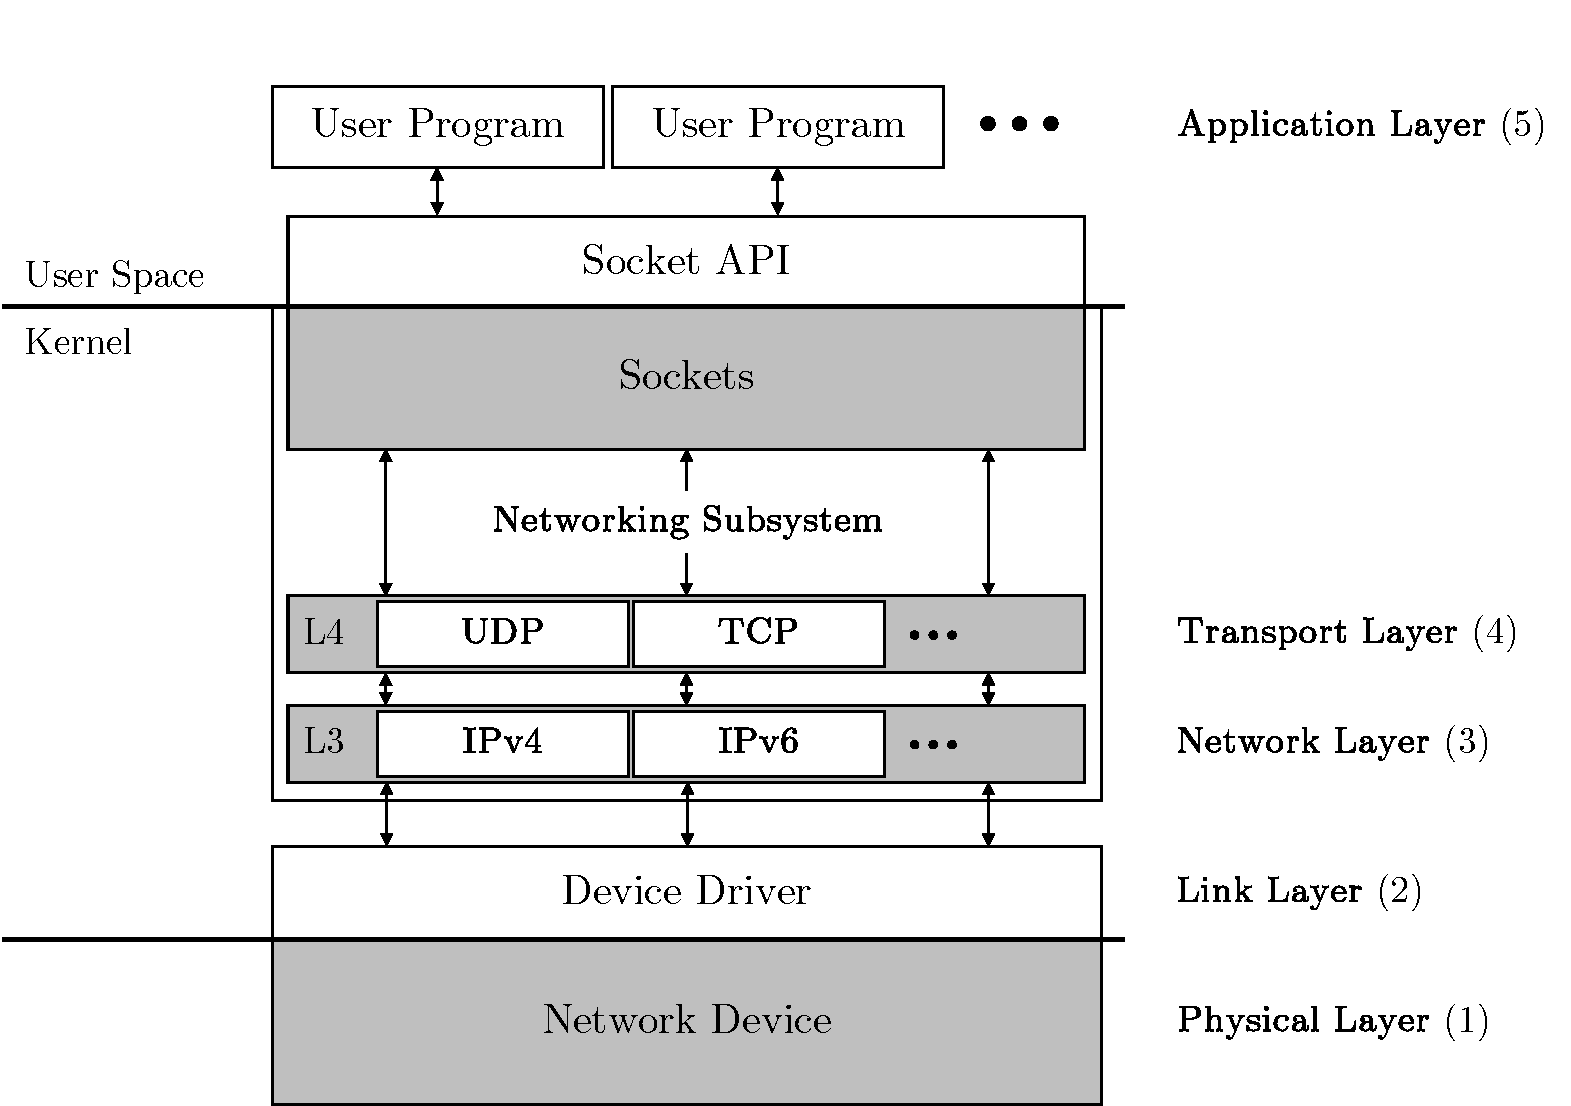
\includegraphics[width=1\linewidth]{figures/linux_nwstack/image03.pdf}
    \caption[Simplified Representation of the Linux Network Stack with associated Layers of the hybrid TCP/IP Reference Model]{Simplified Representation of the Linux Network Stack with associated Layers of the hybrid TCP/IP Reference Model. Adapted from: \cite{lins06}.}
    \label{fig:NWStack}
\end{figure}

Figure \ref{fig:NWStack} presents a simplified schematic of the components of the Linux network stack and how they relate to the layers of the hybrid TCP/IP reference model presented in chapter \ref{chap:RefModel}. This section provides a simplified representation, based on \cite{lins06}, that illustrates the relationship between the components of the network stack. 

First, the components of the network stack will be presented, with a focus on the protocols represented in the TCP/IP reference model. Then, the interaction between the components will be explained by following the path of a packet through the network stack during transmission and reception.


\subsection{Components in the Linux Network Stack}

\subsubsection{Sockets and the Socket API}

Sockets are objects in the operating system that allow data to be exchanged between two applications, usually on a client-server basis. Data can also be exchanged across computer boundaries. Sockets are part of the networking subsystem in the Linux kernel. The socket API represents the associated programming interface \cite{sock01}\cite{sock11}.

Sockets serve as the interface between the application layer and the transport layer in the Linux kernel. Sockets can be defined as the endpoints of a communication channel between two applications. They do not form a separate layer, but allow the application to access the services of the underlying layer, usually the transport layer. The operating system manages all sockets and their associated information \cite{sock02}.

\paragraph{Characteristics of Sockets}

A socket is a generic interface that supports various protocols and protocol families, also known as communication domains. This section focuses on sockets for the TCP/IP protocol family, also known as Internet sockets \cite{like03}.

\subparagraph{Socket Descriptor}
In line with the Linux philosophy of '\textit{everything is a file}', sockets in a system are also represented by an integer, called a socket descriptor in this context. This descriptor can be obtained through a specific call to the operating system and can be used to perform operations such as \texttt{write()} or \texttt{read()}, similar to handling files. Additionally, there are specialized methods like \texttt{send()} or \texttt{receive()} that provide further options.

\subparagraph{Socket Types}
There are different types of sockets that vary in their properties. The two most common types are stream sockets and datagram sockets \cite{like03}.

\begin{itemize}
\item \textbf{Stream sockets} operate in a connection-oriented manner between a client and server application. A connection must be established between the partners before data can be transferred. The TCP protocol is used for this type for Internet sockets.
\item \textbf{Datagram sockets} enable the exchange of individual messages. The sockets operate without a connection. The User Datagram Protocol (UDP) is utilized as the transport layer protocol, resulting in the provision of unreliable transmission.
\end{itemize}

Other socket types, such as Raw sockets or Packet sockets, also exist.


\subparagraph{Socket Address}
A socket can be identified externally using the socket address. In the context of Internet sockets, this address consists of the IP address and a port number and uniquely identifies the socket in the network \cite{sock02}.


\paragraph{Operation of Sockets}

The following section presents important concepts and aspects of working with sockets. The focus is limited to connectionless datagram sockets, as this is the type of socket used in this thesis. For a detailed description of datagram sockets and stream sockets, please refer to \cite{like03}, which serves as the basis for this section.

\begin{figure}[h]
    \centering
    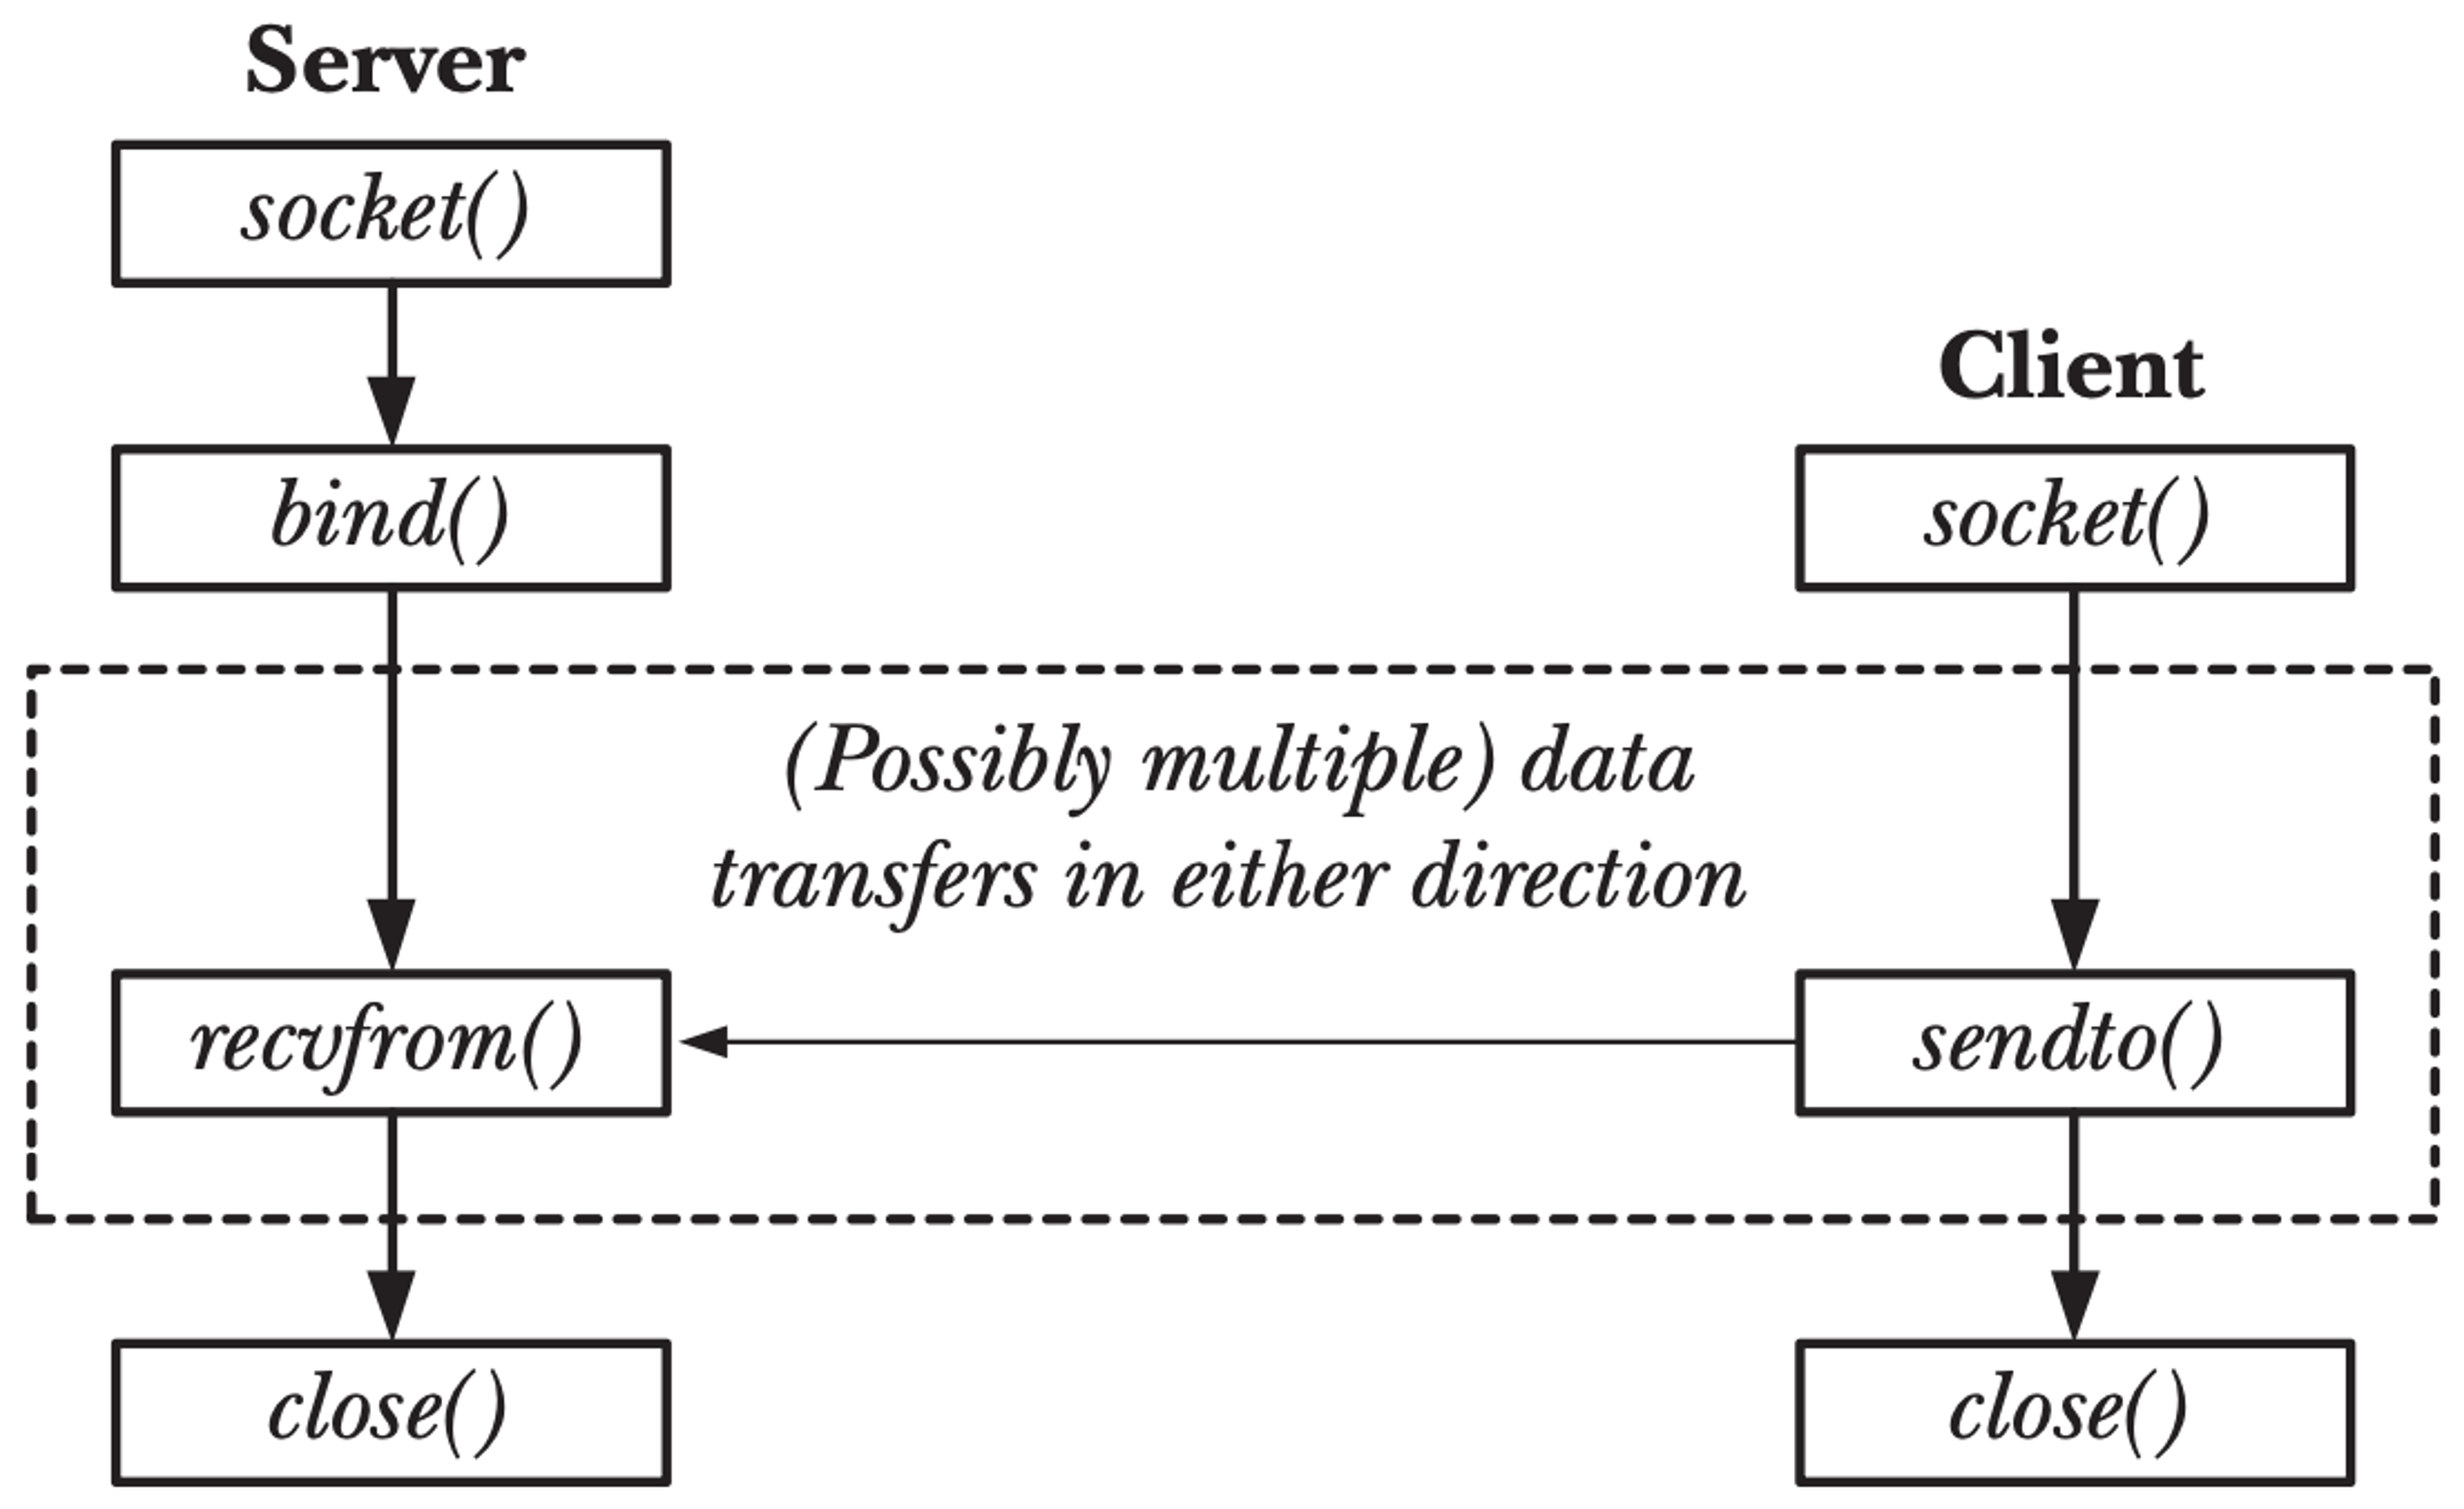
\includegraphics[width=0.75\linewidth]{figures/linux_nwstack/image01.png}
    \caption[Overview of System Calls used with Datagram Sockets]{Overview of System Calls used with Datagram Sockets. Source: \cite{like03}.}
    \label{fig:SocketOperations}
\end{figure}

Figure \ref{fig:SocketOperations} displays the system calls commonly used with a datagram socket for a client-server application. These calls are briefly described below:

\begin{itemize}
\item The \texttt{socket()} call requests the corresponding socket from the operating system, specifying the protocol family and socket type. The return value is the socket descriptor.
\item The \texttt{bind()} call is used to bind the socket to a server address. For Internet sockets, the address consists of the IP address and the port of the server application. This enables the application to receive datagrams sent to this address.
\item The client calls \texttt{sendto()} with both the data to be sent and the address of the socket to which the datagram is to be sent. This call will send the data.
\item \begin{minipage}[t]{\linewidth}
            To receive a datagram, \texttt{recvfrom()} is called. The argument can be used to specify the address of the sender's socket from which the data is to be received. If no restrictions should be defined for the sender's address, \texttt{recv()} can also be used.\\
            Both calls save exactly one received datagram in a buffer, a pointer to which is also passed as an argument to the function. If no data has been received when \texttt{recv()} or \texttt{recvfrom()} is called, the call is blocked.\\
            If multiple datagrams are received, they are stored in the receive buffer of the corresponding socket. However, when one of these functions is called, only one message is passed to the application via the socket.
      \end{minipage}
\item If the socket is no longer needed, it can be closed using \texttt{close()}.
\end{itemize}


\paragraph{Raw Sockets and Packet Sockets}

Raw sockets and Packet sockets are additional types of Internet sockets. These are an addition to the stream and datagram sockets already mentioned and allow access to lower layers of the network stack instead of hiding them from the user \cite{sock07}.

\begin{figure}[h]
    \centering
    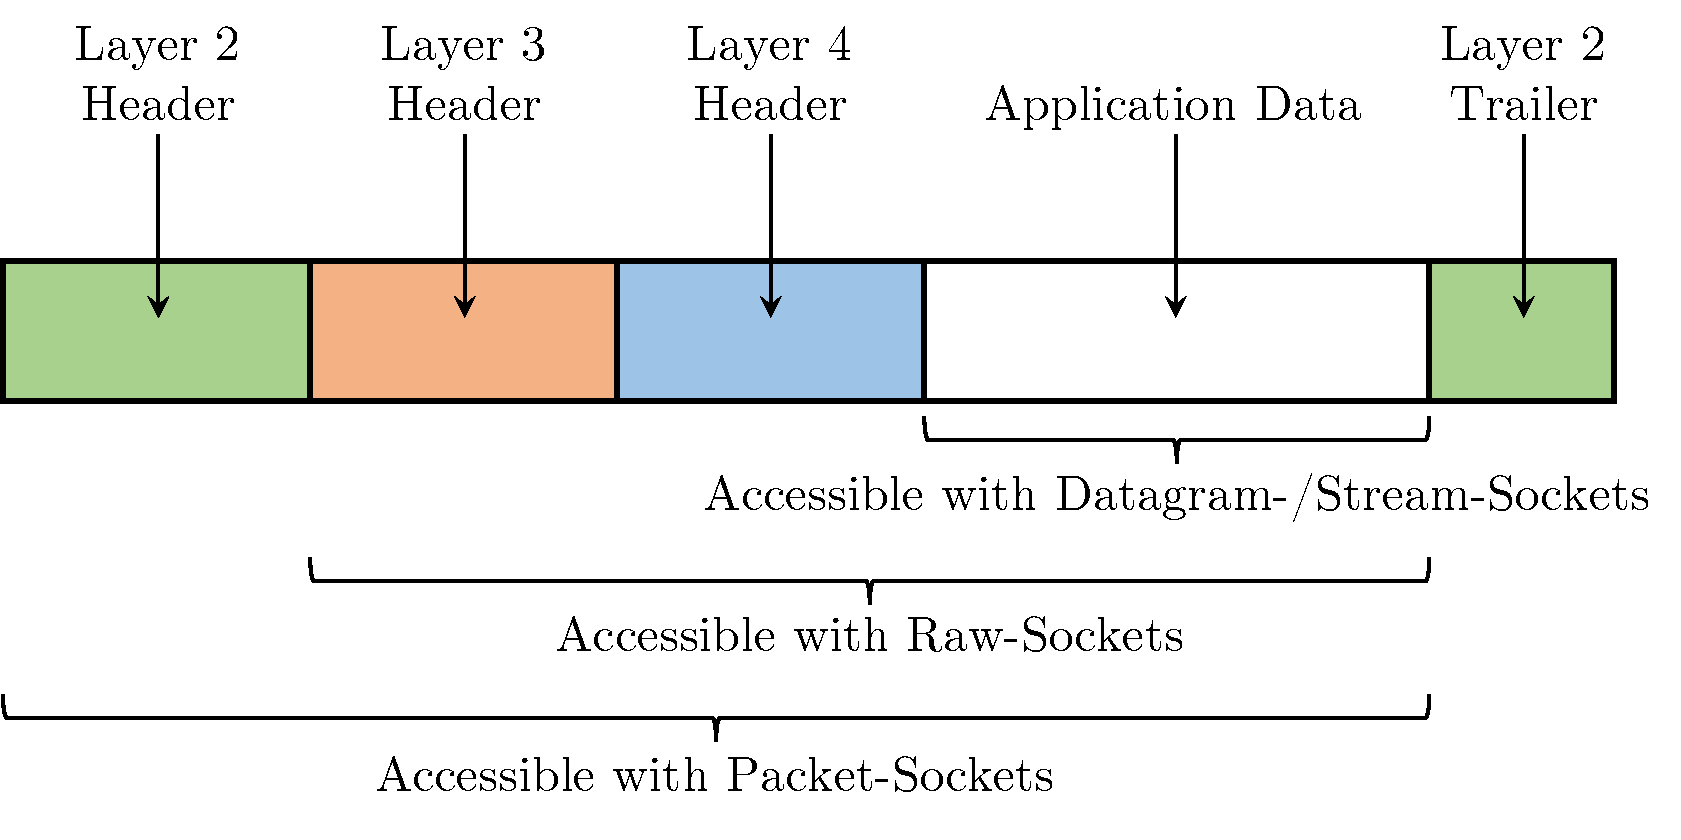
\includegraphics[width=0.9\linewidth]{figures/linux_nwstack/image02.pdf}
    \caption[Overview of Network Layers and Access Possibilities with different Socket Types]{Overview of Network Layers and Access Possibilities with different Socket Types. Adapted from: \cite{sock07}.}
    \label{fig:SocketAccessPossib}
\end{figure}

Figure \ref{fig:SocketAccessPossib} displays the access possibilities with different socket types. Raw sockets provide access to the transport layer (4) and network layer (3) of the network stack \cite{sock08}, including TCP or UDP as well as IP in the case of the TCP/IP reference model. Packet sockets can also be utilized to access the link layer (2), enabling access to almost the entire Ethernet frame, except for the preamble and trailer \cite{sock09}.

The concept underlying Raw and Packet sockets involves the implementation of separate protocol layers in the application. Depending on the chosen socket type, the application can implement layers 2 to 4 \cite{sock08}. Furthermore, Packet sockets can also be used to capture the entire communication of a system, as used by Wireshark, for example.

Raw or Packet sockets eliminate the overhead of the respective protocol layer in the Linux kernel, which can potentially accelerate processing. They also increase flexibility, as certain fields in the header can be easily modified.

A disadvantage, however, is that in order to maintain compatibility with other TCP/IP implementations, the corresponding protocols must be fully and correctly implemented in the application. Additionally, using Raw or Packet sockets requires that the application be executed with root privileges.

The technical report 'Introduction to RAW sockets' \cite{sock07} provides a comprehensive overview of Raw and Packet sockets and their application. This report was also used for programming in this thesis.



\subsubsection{Layers 3 and 4 in the Networking Subsystem}
The networking subsystem of the Linux kernel includes not only sockets but also layers 3 and 4, namely the transport and network layers. These layers implement the protocols described in \label{chap:ProtosRefModel}, while sockets provide an interface between the application and the network stack.

\paragraph{Protocol Handler}
The corresponding protocols are implemented in layers 3 and 4, including implementations for protocols from the TCP/IP reference model and other protocols in their respective layers. It is also possible to develop handlers for your own protocols \cite{lins06}.

An important task in the network subsystem is to execute the correct protocol handler for the corresponding layer. For outgoing packets, this is determined by the socket. For instance, an Internet socket that uses the datagram type employs the UDP protocol at layer 4 and the IPv4 protocol at layer 3. The protocol handler to be executed for incoming packets is determined from the header of the underlying layer. Both the Ethernet header and the IP header contain a corresponding field for the service-using protocol \cite{lins06}.

The protocol handlers of the respective layer implement the standardized behavior for this protocol. These are described in the chapter \label{chap:ProtosRefModel}. Implementation details will not be discussed further at this point. For more information, please refer to \cite{lins01}.

\paragraph{Data Structures in the Networking Subsystem of the Linux Kernel}
This chapter presents two significant data structures of the networking subsystem in the Linux kernel, as described in \cite{lins06}.

\subparagraph{Socket Buffer Structure}
The socket buffer structure, also known as \texttt{sk\_buff}, is the most important data structure in the network stack. It represents a packet that has been received or is to be sent and is used by layers 2, 3, and 4. This structure eliminates the need to copy packet data between layers.

The structure contains control information associated with a network packet, but not the actual data itself. Included in this structure are:

\begin{itemize}
\item Information on the organization of the socket buffers by the kernel
\item Pointers to the data and to the headers of layers 2, 3 and 4
\item Length of the data and the headers
\item Data on the internal coordination of the packet
\item Information on the associated network device (see \ref{chap:netdevice})
\end{itemize}

The mentioned pointers to the data point to a data field associated with the socket buffer. This field contains the packet data and associated headers and is created when a socket buffer is allocated. The socket buffer has pointers to different locations in this data field, depending on the layer currently using the socket buffer.

Additionally, there are management functions related to the socket buffers. These functions can be utilized by individual network layers to add or remove their headers to the packet during processing. There are also functions to modify the size of the data field.

\subparagraph{Network Device Structure} \label{chap:netdevice}
The network device structure, also known as \texttt{net\_device}, contains information about a specific network interface. This structure is present in the kernel for every network interface of the system.

Some important fields of this structure are (according to \cite{lins01}):
\begin{itemize}
\item Identifier of the interface
\item MTU of the network interface
\item MAC address of the interface
\item Configurations and flags of the interface
\item Pointer to the transmit method of the interface
\end{itemize}

\subsubsection{Network Device and Device Driver}
The network device, also known as the network interface, along with its associated device driver, is the lowest component in the Linux network stack. The device driver performs the tasks of layer 2 of the TCP/IP reference model, while the network interface physically transmits the data, working on layer 1 of the reference model \cite{lins01}.

The main tasks of the device driver are to receive packets addressed to the system and forward them to layer 3 of the network stack, and to send packets generated by the system.

The driver interacts with the network interface, which transmits the data according to the respective transmission standard \cite{lins01}. To exchange data with the interface, the driver creates two ring buffers: the TX\_Ring and the RX\_Ring, which are used for sending and receiving data. These buffers are located in the system memory and contain a fixed number of descriptors pointing to buffers where packets can be stored. They are empty during initialization and accessed by the interface via DMA \cite{lins03, lins14}.

The implementation of the driver depends on the hardware and is therefore not standardized. However, the Linux kernel defines how the driver interacts with the networking subsystem.

\subsection{Path of a Network Packet} \label{chap:sedrecpath}
This section explains how a packet travels through the Linux network stack by examining the interactions of the components described above. Specifically, this section will focus on the reception and transmission of a UDP packet.

The following overview provides a general understanding of the process and will serve as a foundation. For a more detailed explanation of the packet's path, please refer to \cite{lins01} and \cite{lins06}.

\subsubsection{Receiving a Packet} \label{chap:recpath}
When a frame is received by the network card, it first checks for errors using the Ethernet frame checksum and then verifies if it is intended for the network interface by using the MAC address. The frame is then written to a free buffer in the RX\_Ring via DMA, which was created by the device driver during initialization. If no buffers are available, the frame is dropped \cite{lins03, lins06, lins14}.

Interrupts are utilized to notify the system about a packet. Different strategies can be employed for this purpose. In the simplest case, a hardware interrupt is triggered for each received frame \cite{lins06}.

To minimize processing in the interrupt context, softirqs are utilized \cite{lins03}. Softirqs are non-urgent interruptible functions in the Linux kernel that are designed to handle tasks that do not need to be done in the interrupt context. The handlers for the softirqs are executed by ksoftirq kernel threads, with one thread for each CPU core on the system \cite{like02}.

The network driver's hardware interrupt handler schedules a softirq to process packets for the device by adding the it to a poll list. When the corresponding softirq kernel thread is scheduled, it executes the function \texttt{net\_rx\_action} \cite{lins03}.

This function, executed in the context a softirq, processes all devices in the poll list. During the processing of the RX\_Ring of a network device, the hardware interrupts for this device are deactivated. Each  packet is wrapped in an \texttt{sk\_buff} structure and handled by an appropriate Layer 3 protocol handler. In the case of IP packets, the \texttt{ip\_rcv()} function is used. The process is repeated until there are no frames left in the RX\_Ring of the Interface or until a limit, called device weight, is reached. Additionally, a new descriptors are allocated and added to the RX\_Ring \cite{lins03, lins13, lins14}.

The \texttt{ip\_rcv()} function processes the packets as defined in the protocol, including defragmentation and routing. It then calls the appropriate protocol handler of the layer above. For UDP, this is \texttt{udp\_rcv()} \cite{lins01}.

During processing by UDP, the system verifies the availability of a socket with the corresponding port number. If available, the packet is copied into the receive buffer of the socket. If no corresponding socket is found, the packet is dropped \cite{lins01}.

Processing of the packet in the context of the softirq is now complete. The application can retrieve the packet from the receive buffer of the socket using the \texttt{receive()} call.


\subsubsection{Sending a Packet}
To send a packet, an application needs an appropriate socket, in the case of UDP packets an Internet socket of type datagram. The \texttt{sendto()} function is used to send the data, which contains the actual data as well as the address of the socket to which the data should be sent.

In the Linux kernel, calls to \texttt{sendto()} for a UDP socket are handled by the \texttt{udp\_sendmsg()} function in context of the application. This creates a socket buffer for the packet. Additionally, the UDP packet undergoes initial checks such as the compliance with the maximum length, and the UDP header is generated. Subsequently, the packet is forwarded to the IP protocol handler \cite{lins01}.

The Internet Protocol handler generates the IP header and fragments the packet if required. In addition, the protocol handler performs routing to determine which network device the packet should be sent to. This process is also performed in the context of the application \cite{lins01, lins03}.

To implement traffic management and prioritization, a layer called queueing discipline (QDisc) is placed between the protocol handler of layer 3 and the device driver. By default, a QDisc called 'pfifo\_fast' is used, which is essentially a FIFO queue. The queuing of the packet is also handled in the context of the application \cite{lins03, lins12}.

The actual transmission of the packet over the network interface card is usually done in the context of a softirq. The device driver for the interface adds the Ethernet header and places it in the transmission queue of the interface, known as the TX\_Ring. The NIC hardware then fetches the packets from the TX\_Ring using DMA and transmits them over the physical medium. An interrupt is generated by the interface to indicate a successful transmission \cite{lins06, lins14}.




\section{Advanced Networking Options}

\subsection{Hardware Offloading} \label{chap:HWOffload}
Hardware offloading enables specialized hardware to perform compute-intensive tasks instead of the system's CPU, reducing its workload. The workload for the CPU is reduced by utilizing specialized In terms of networking, this specialized hardware is integrated into the network interface \cite{tuning01}. Linux distinguishes between two types of offload: Checksum Offload and Segmentation Offload \cite{tuning02, tuning03}.

Checksum Offload refers to the ability to calculate various checksums of the protocols in the TCP/IP reference model, including the checksum in the Ethernet frame and the checksum in the IP or UDP header \cite{tuning02}.

Segmentation Offload can be used to fragment a UDP packet using the network interface. A similar technique also exists for TCP \cite{tuning03}.


\subsection{Receive Side Scaling} \label{chap:ReceiveSideScaling}
Receive Side Scaling, or RSS for short, is a technology used to improve network performance. The procedure for receiving a packet is described in \ref{chap:recpath}. The interrupt and softirq described there, which carry out the processing of the received packet, are handled by a single CPU \cite{rss01}.

The concept behind RSS is to distribute network data processing across multiple CPU cores instead of keeping it confined to a single core. Incoming network packets are distributed to different processor cores based on a hash function \cite{rss02}.

For Intel network cards, the hash is calculated based on the packet type. The network interface parses all packet headers and uses specific fields as input values for the hash function. In the case of a non-fragmented UDP packet, the destination and source IP addresses, along with the destination and source port, are used to calculate a 32-bit hash value. This hash value determines the queue and CPU core for processing the packet. All packets with the same input parameters are considered a related communication flow and have the same hash value. As a result, they are processed by the same CPU \cite{rss03}.

\subsection{Interrupt Moderation} \label{chap:InterMod}
As explained in \ref{chap:sedrecpath}, the system generates an interrupt for both incoming and outgoing packets, which can negatively impact performance, particularly at high transmission rates due to the high number of interrupts generated \cite{intermod01}. Interrupt moderation can be used to mitigate this issue by delaying the generation of interrupts until multiple packets have been sent or received, or a timeout has occurred, thereby reducing CPU utilization \cite{intermod02}.

The Intel network interface drivers enable the configuration of a fixed timeout value for interrupt moderation or the complete deactivation of interrupt moderation. By default, adaptive interrupt moderation is active, which, according to Intel, provides a balanced approach between low CPU utilization and high performance \cite{intermod03}. The interrupt rate is dynamically set based on the number of packets, packet size, and number of connections. The associated patent \cite{intermod04} provides a detailed description of this process. Typically, the interrupt rate is set to achieve either low latency or high throughput, depending on the type of traffic. For small datagrams, a low interrupt rate (i.e., a high number of interrupts/s) is selected, while for large datagrams, a high interrupt rate (i.e., a lower number of interrupts/s) is selected. Additionally, the interrupt rate also depends on the number of connections, with a high interrupt rate selected for a low number of connections and a low interrupt rate selected for a high number of connections.

The interrupt moderation rate of Intel network interfaces can be configured using the 'ethtool' configuration tool within the range of 0 to 235 µs. A value of 0 µs deactivates interrupt moderation.

\subsection{Quality of Service} \label{background:tuning:qualityofservice}
Quality of Service (QoS) comprises different mechanisms to provide distinct service levels for various network traffic. A service level includes statements about bandwidth, jitter, or reliability \cite{qos01}. To achieve a service level, QoS consists of various components and measures, including packet marking methods, traffic shaping methods, and the implementation of various queues in network devices \cite{qos02}. Due to the broad scope of Quality of Service and its related technologies, this section only briefly introduces key technologies used.

One way to classify traffic is by using the Differentiated Services field in the IP header (refer to \ref{chap:ipheader}). This field enables the specification of a Differentiated Services Field Codepoint, which can be interpreted as a priority. The values range from 0 to 63, with 63 being the highest priority \cite{qos02}.

Differentiated Services Field Codepoints are solely used for packet classification. To achieve specific service levels in the network, it is necessary to configure the network hardware to ensure the desired traffic handling. This may involve prioritizing certain Differentiated Services Field Codepoint values over others \cite{qos02}.


    \chapter{Methodology}

\section{Setup}
\subsection{Hardware Setup}

\subsubsection{Computer Systems}
The test setup consisted of five computer systems, which can be classified into three types.  Specifically, there were two 'High-Performance PCs' (HPC1 and HPC2), two 'Traffic PCs' (TPC1 and TPC2), and one system from the Concurrent iHawk platform.

\paragraph{Hardware of the Computer System Types} \label{chap:ComputerHardware}
Table \ref{hwtable} provides an overview of the hardware of the computer system types used. The hardware was intentionally chosen to represent different performance classes in order to identify possible limitations during the tests.

Table \ref{hw:hpc} shows that the High-Performance PCs use an Intel Core i9 13900 CPU with Intel Hybrid Technology, providing 8 Performance-Cores and 16 Efficient-Cores \cite{setup10}. However, due to incompatibility with the operating system, the efficient cores are disabled, resulting in the use of 8 physical cores or 16 logical cores for systems of this type.

\begin{table}[h!]
\centering
\newcolumntype{C}[1]{>{\raggedright\arraybackslash}p{#1}}

\begin{subtable}{\linewidth}
\centering
\begin{tabular}{C{2.2cm} | C{5.1cm}}
	\toprule
	\textbf{Category} & \textbf{Hardware}\\
	\midrule
	CPU & Intel Core i9 13900\\
	RAM & 32 GB DDR5 6400 MHz\\
	Mainbaord & ASUS PRIME Z790-P WIFI\\
	Disk & 2 TB NVMe M.2 SSD\\
	\bottomrule
\end{tabular}
\caption{High-Performance PC}
\label{hw:hpc}
\end{subtable}
\vspace{6pt}

\begin{subtable}{\linewidth}
\centering
\begin{tabular}{C{2.2cm} | C{5.1cm}}
	\toprule
	\textbf{Category} & \textbf{Hardware}\\
	\midrule
	CPU & Intel Core i7-3770S\\
	RAM & 16 GB DDR3 1333 MHz\\
	Mainbaord & GA-Z77X-UD5H (TPC1), GA-Z77X-UD3H (TPC2)\\
	Disk & 256 GB SATA III SSD\\
	\bottomrule
\end{tabular}
\caption{Traffic PC}
\label{hw:tpc}
\end{subtable}
\vspace{6pt}

\begin{subtable}{\linewidth}
\centering
\begin{tabular}{C{2.2cm} | C{5.1cm}}
	\toprule
	\textbf{Category} & \textbf{Hardware}\\
	\midrule
	CPU & \textbf{2x} Intel Xeon Gold 6234\\
	RAM & 48 GB  DDR4 2400 MHz\\
	Mainbaord & Supermicro X11-DPi-N\\
	Disk & 2 TB HDD\\
	\bottomrule
\end{tabular}
\caption{iHawk}
\label{hw:ihawk}
\end{subtable}

\caption{Overview of the Hardware of the Computer Systen Types}
\label{hwtable}
\end{table}




\paragraph{Comparison with Computer Systems in the Test Support System}
When selecting the hardware, care was taken to ensure that it was similar or identical to the hardware used in a Distributed Test Support System.

\subparagraph{Systems of the Type 'Traffic PC'}
The 'Traffic PC' systems used in this context are similar to the I/O PCs used in the Distributed Test Support System. The I/O PCs are based on the CompactPCI Serial architecture, which enables modular systems consisting of a system module containing the CPU and up to eight peripheral modules connected to the system module via PCI Express. \cite{setup01}.

The SC5-FESTIVAL card manufactured by EKF Elektronik GmbH serves as the system module in the Distributed Test Support System. It is equipped with an Intel Core i3 7100E processor \cite{setup02}, which provides comparable performance to the Intel Core i7-3770S used in the Traffic PCs \cite{setup03}.

\subparagraph{iHawk Platform}
iHawk is a computer platform manufactured by Concurrent that is designed with a focus on time-critical simulation or data acquisition \cite{setup04}. The system used for the tests in this thesis, with the data described in Table \ref{hw:ihawk}, will also be used with the same configuration in a Distributed Test Support System. This ensures that the conditions of the tests carried out here are comparable to those of the Distributed Test Support System.


\paragraph{Characteristics of the used iHawk System} \label{chap:iHawkChar}
In the following, the special features of the iHawk system used, which were taken into account in the analyses carried out with special test scenarios, will be discussed.

\begin{figure}[ht!]
    \centering
    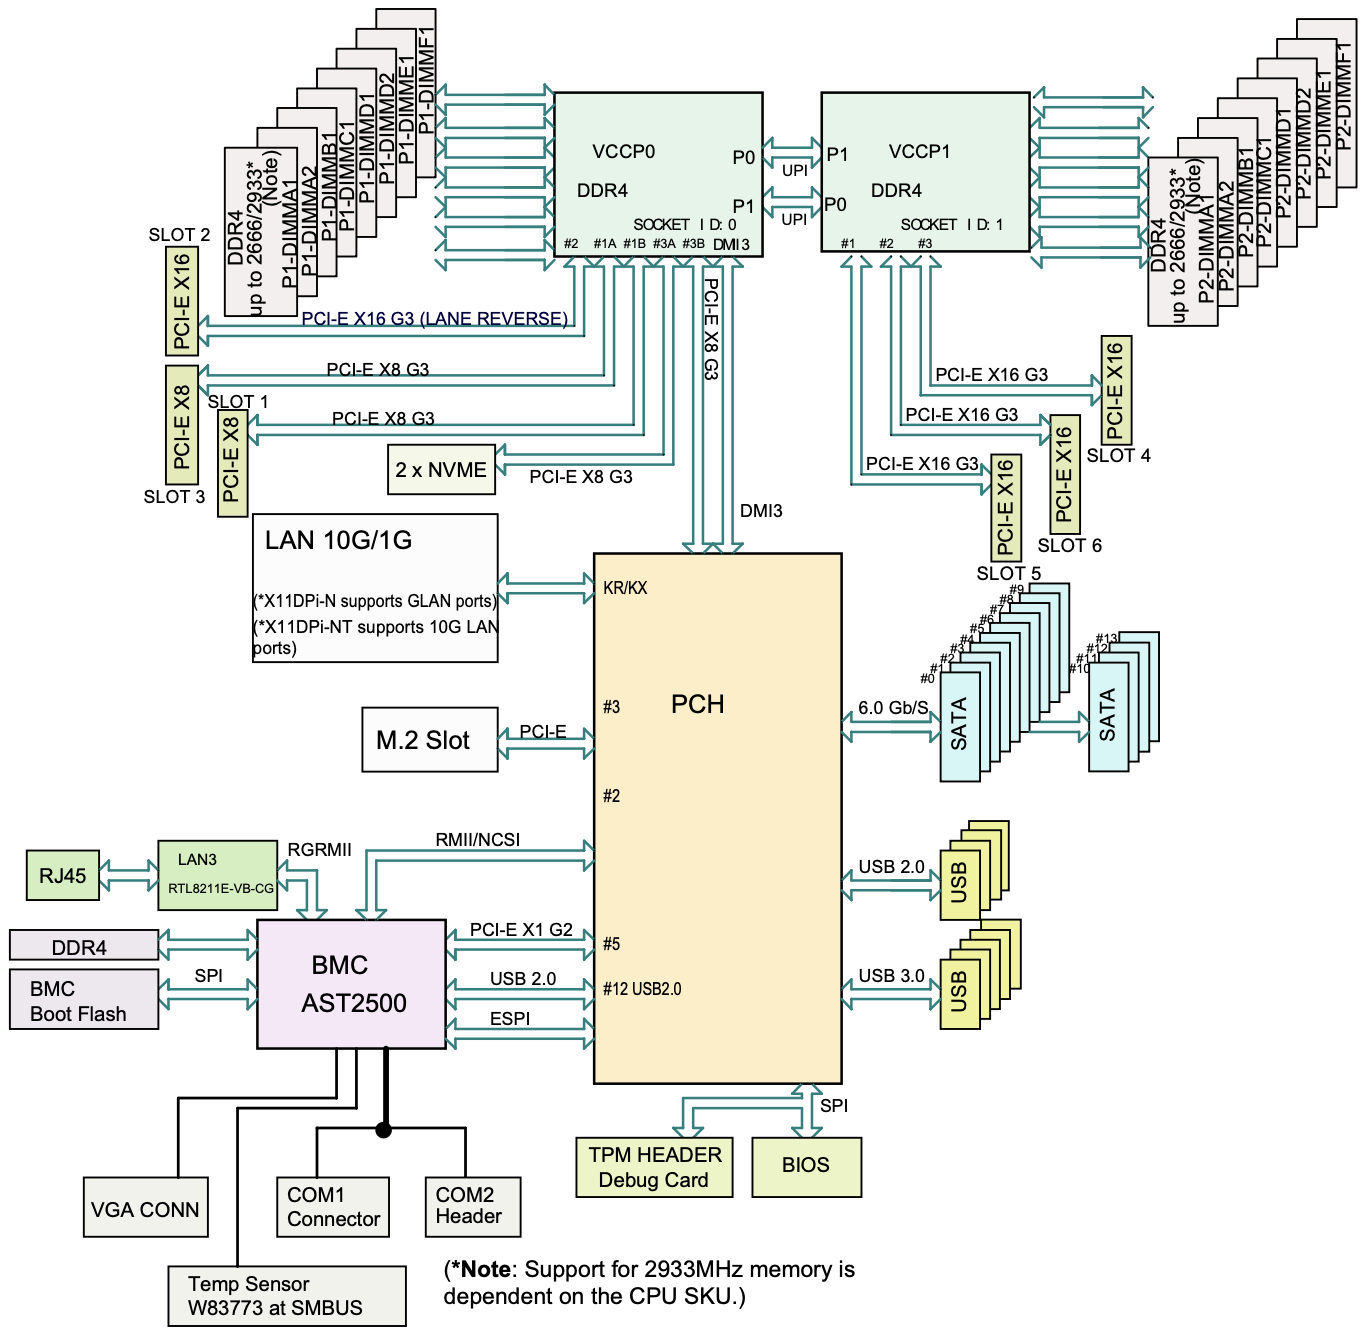
\includegraphics[width=1\linewidth]{figures/method/image1.png}
    \caption[Block Diagram of the Supermicro X11-DPi-N Mainboard]{Block Diagram of the Supermicro X11-DPi-N Mainboard. Source: \cite{setup05}.}
    \label{fig:BlockDiagrIHawk}
\end{figure}

The iHawk is a dual-socket system, as shown in the block diagram (Figure \ref{fig:BlockDiagrIHawk}). It utilizes a NUMA (Non-Uniform Memory Access) memory design, which means that memory performance varies at different points in the address space, depending on whether it is local memory or the memory of the other processor. Typically, access to local memory is significantly faster than to the memory of the other processor. A CPU with its local memory and access to remote memory is referred to as a NUMA node \cite{setup06}.

To access the memory of the other NUMA node, an interconnect between the sockets is used. This can lead to potential problems such as:

\begin{itemize}
\item Increase in latency for memory access
\item Throughput bottleneck
\end{itemize}

The iHawk system utilizes two Intel Ultra Path Interconnect (UPI) links, as illustrated in Figure \ref{fig:BlockDiagrIHawk}. Each link operates at a speed of 10.4 GT/s, providing a total full-duplex bandwidth (two links in two directions) of 41.6 GByte/s \cite{setup08}. Accessing memory from the other NUMA node via the UPI increases latency by approximately 50\% \cite{setup06}, resulting in a memory latency of around 130 ns \cite{setup07} between the two sockets.

The block diagram shows that each PCI Express slot is connected to one CPU. Slots 0 to 3 are connected to CPU 0, while slots 4 to 6 are connected to CPU 1. It is important to note that the problems previously described for memory accesses also apply to accessing PCI Express devices on the other NUMA node, as they are also carried out via the UPI links.


\subsubsection{Network Hardware}

\paragraph{Ethernet Switch} \label{chap:EthernetSwitch}
The Ethernet switch used is a Cisco CBS350-8XT from the Cisco Business 350 series. It is a Layer 3 managed switch that supports 10 GbE. Its specifications are as follows \cite{setup09}:

\begin{itemize}
\item 8x RJ45 10 GbE Ports
\item 2x SPF+ (shared with RJ45 Port)
\item 160 GBit/s switching capacity
\item 6 MB packet buffer dynamically shared across all ports
\item Quality of Service (QoS) with 8 hardware queues
\item Support for jumbo frames with a maximum size of 9000 bytes
\end{itemize}

The Cisco CBS350-8XT is a Layer 3 switch that can forward packets based on both MAC and IP addresses, similar to a router.  However, for the purposes of the tests conducted in this thesis, this functionality was not required, so the switch was configured as a Layer 2 switch.

\paragraph{Network Interface Cards} \label{chap:NicTypes}

The tests only use PCIe Network Interface Cards (NIC) that are capable of 10 GbE. The main types of network interfaces used are Intel's X520-DA2, X540-T2, and X710-T2L. Network interfaces from Lenovo and Inspur are also considered. Table \ref{tab:NWHardware} provides a concise overview of the network interfaces used according to \cite{setupnw01, setupnw02, setupnw03, setupnw04}. All interface cards support the same offloading mechanisms regarding UDP (see \ref{chap:HWOffload}). \\

{
\renewcommand{\arraystretch}{1.3}

\begin{table}[h!]
\centering
\newcolumntype{C}[1]{>{\raggedright\arraybackslash}p{#1}}

\begin{subtable}{\linewidth}
\begin{tabularx}{\textwidth}{C{2.2cm} | X | X | X}
	\toprule
	& \textbf{Intel X520-DA2} & \textbf{Intel X540-T2} & \textbf{Intel X710-T2L}\\
	\midrule
	Year & 2009 & 2012 & 2019\\
	Ports & Dual (SPF+) & Dual (RJ45) & Dual (RJ45)\\
	System Interface & PCIe v2.0 (5 GT/s), x8 Lane & PCIe v2.0 (5 GT/s), x8 Lane & PCIe v3.0 (8 GT/s), x8 Lane\\
	Controller & Intel 82599 & Intel X540 & Intel X710-AT2\\
	Data Rate & max. 10 GBit/s & max. 10 GBit/s & max. 10 GBit/s \\
	\bottomrule
\end{tabularx}
\end{subtable}
\vspace{6pt}

\begin{subtable}{\linewidth}
\begin{tabular}{C{2.2cm} | C{3.6cm} | C{3.6cm}}
	\toprule
	& \textbf{Inspur X540-T2} & \textbf{Lenovo QL41134}\\
	\midrule
	Year & - {\footnotesize{\textit{(unknown)}}} & 2021\\
	Ports & Dual (RJ45) & 4 (RJ45)\\
	System Interface & PCIe v2.0 (5 GT/s), x8 Lane & PCIe v3.0 (8 GT/s), x8 Lane\\
	Controller & Intel X540 & QLogic QL41134\\
	Data Rate & max. 10 GBit/s & max. 10 GBit/s \\
	\bottomrule
\end{tabular}
\end{subtable}

\caption{Overview of the Specifications of the Network Interface Cards}
\label{tab:NWHardware}
\end{table}
}


The network interfaces were selected broadly to reduce dependence on specific interfaces or manufacturers. Additionally, network cards of varying ages and prices were considered to account for potential hardware limitations.

Chapter \ref{chap:Architectures} explains for each topology which network interfaces are used on which computer system. It should be noted that the Intel X710-T2L network interfaces are not compatible with computer systems of the 'Traffic PC' type.


\subparagraph{Comparison with Network Interfaces in the Test Support System}

In the Distributed Test Support System, for systems similar to the 'High Performance PCs' and the iHawk, a wide range of PCIe 10GbE network interfaces can be used. However, the CompactPCI Serial systems can only use network interfaces for which a corresponding peripheral module is available.

The Distributed Test Support System utilizes the SN5-TOMBACK peripheral module from EKF \cite{setupnw05}. This module uses the Intel 82599 controller, has two SPF+ ports and supports 10 GbE. It is therefore comparable to the Intel X520-DA2 network card in the test setup, which uses the same controller.

\paragraph{Cabling}
The cabling of the hardware used was carried out using Cat7 Ethernet patch cables with RJ45 plugs or with fiber optic cables and Intel SPF+ SR modules. Both cabling systems used are suitable for 10 GbE.

\subsection{Software Setup}
This chapter describes the software versions and important configurations used in the test setup.

\subsubsection{Versions}
\paragraph{Operating System}
The operating system used on all computer systems is the real-time operating system RedHawk Linux 9.2 based on Ubuntu 22.04.3 LTS.

\begin{itemize}
\item \textbf{Operating System:} RedHawk 9.2 with Ubuntu 22.04.3 LTS user environment
\item \textbf{Linux Kernel:} 6.1.19-rt8-RedHawk-9.2-trace
\end{itemize}

RedHawk Linux 9.2 is a real-time operating system developed by Concurrent, optimized for real-time determinism with precise and consistent response times and low latency \cite{swsetup01}. The manufacturer integrates open source patches and proprietary enhancements into the Linux kernel. The following list briefly describes some important features of the real-time optimized Linux kernel from the product brochure \cite{swsetup02}:

\begin{itemize}
\item \textbf{Standard Linux API}: Since RedHawk is based on a Linux kernel, it offers all standard Linux user level APIs such as POSIX. Therefore, applications created for other Linux distributions can also be executed on the operating system.
\item \textbf{Frequency-Based Scheduling}: RedHawk has a Frequency-Based Scheduler, which allows processes to be executed in a cyclical execution pattern driven from a real-time clock.
\item \textbf{Processor Schielding}: RedHawk enables the shielding of individual cores from timers, interrupts, or other Linux tasks, providing a deterministic execution environment.
\item \textbf{Multithreading and Preemption}: RedHawk allows multiple processes to execute simultaneously in the kernel while protecting critical data or code sections with semaphores or spinlocks. In the RedHawk kernel, processes can be preemptively interrupted to reallocate CPU control from a lower-priority to a higher-priority process, except during execution in critical kernel sections. To ensure deterministic responses, critical sections of the kernel have been optimized to reduce non-preemptable conditions and enabling high-priority processes to immediately respond to external events, even when the CPU is actively engaged.
\end{itemize}

RedHawk Linux was chosen for the test setup as it is also used in the Distributed Test Support System. It also offers low latency, which should have a positive impact on the performance characteristics.

\paragraph{Drivers of the Network Interface Cards}

The drivers supplied with the kernel are used for the network cards. Table \ref{tab:drivernic} lists the drivers used for the network cards.

\begin{table}[h]
\centering
\begin{tabular}{l|l}
	\toprule
	\textbf{Driver} & \textbf{Network Interface Card}\\
	\midrule
	i40e & Intel X710-T2L\\
	ixgbe & Intel X520-DA2, Intel X540-T2, Inspur X540-T2 \\
	qede & Lenovo QL41134\\
	\bottomrule
\end{tabular}
\caption{Overview of the Drivers of and the associated Network Interface Cards.}
\label{tab:drivernic}
\end{table}

\subsubsection{Configurations}

\paragraph{Activation of Jumbo Frames}

The tests used jumbo frames with a maximum size of 9000 bytes. Jumbo frames must be supported by all network nodes to avoid packet loss \cite{swsetup04}. Since the network in the test setup and also in the Distributed Test Support System is completely under user control, no problems are expected in this regard. \\

\begin{lstlisting}[language=Bash, caption=Configuration of Jumbo Frames for the ethX Interface., label=lst:jumbocongif]
ifconfig ethX mtu 9000
\end{lstlisting}

Listing \ref{lst:jumbocongif} shows the configuration of jumbo frames with a maximum size of 9000 bytes for the \textit{ethX} interface.


\paragraph{Real-time Process} \label{chap:RTProcess}
The tests, specifically the test program described in the following section \ref{chap:TestSuite}, were executed as a real-time process with the highest priority. This was done in order to obtain realistic test conditions, as the communication layer is also executed as a real-time process in the Distributed Test Support System. \\

\begin{lstlisting}[language=Bash, caption=Modification of the real-time Attributes of a Process., label=lst:rtprocess]
chrt -f -p 99 [PID]
\end{lstlisting}

Listing \ref{lst:rtprocess} contains the command used to modify the real-time attributes of a process with a specific PID (Process ID). The same command was also applied to the test program. According to \cite{swsetup05}, the real-time attributes were modified as follows:

\begin{itemize}
\item Change of the \textbf{scheduling policy} to \texttt{SCHED\_FIFO}. This is a real-time scheduling policy where each thread is assigned a fixed priority between 1 and 99, with higher numbers indicating higher priority. The policy is non-preemptive, which means the threads run until they block, yield, or are preempted by a higher priority thread. For threads with the same priority, the one waiting the longest runs next, adhering to a first in first out (FIFO) order \cite{swsetup06}.
\item Change of the \textbf{scheduling priority} to 99, which is the highest priority of \texttt{SCHED\_FIFO} \cite{swsetup06}.
\end{itemize}

\clearpage

\section{Network Topologies} \label{chap:Architectures}
For the tests with the described setup, two different topologies were utilized for the local Ethernet network and the arrangement of the computer systems. Both topologies are star-shaped, consisting of bidirectional point-to-point links that connect two systems. Each link can be used independently in both directions \cite{Tanenbaum2010}.


\begin{figure}[h]
    \centering
    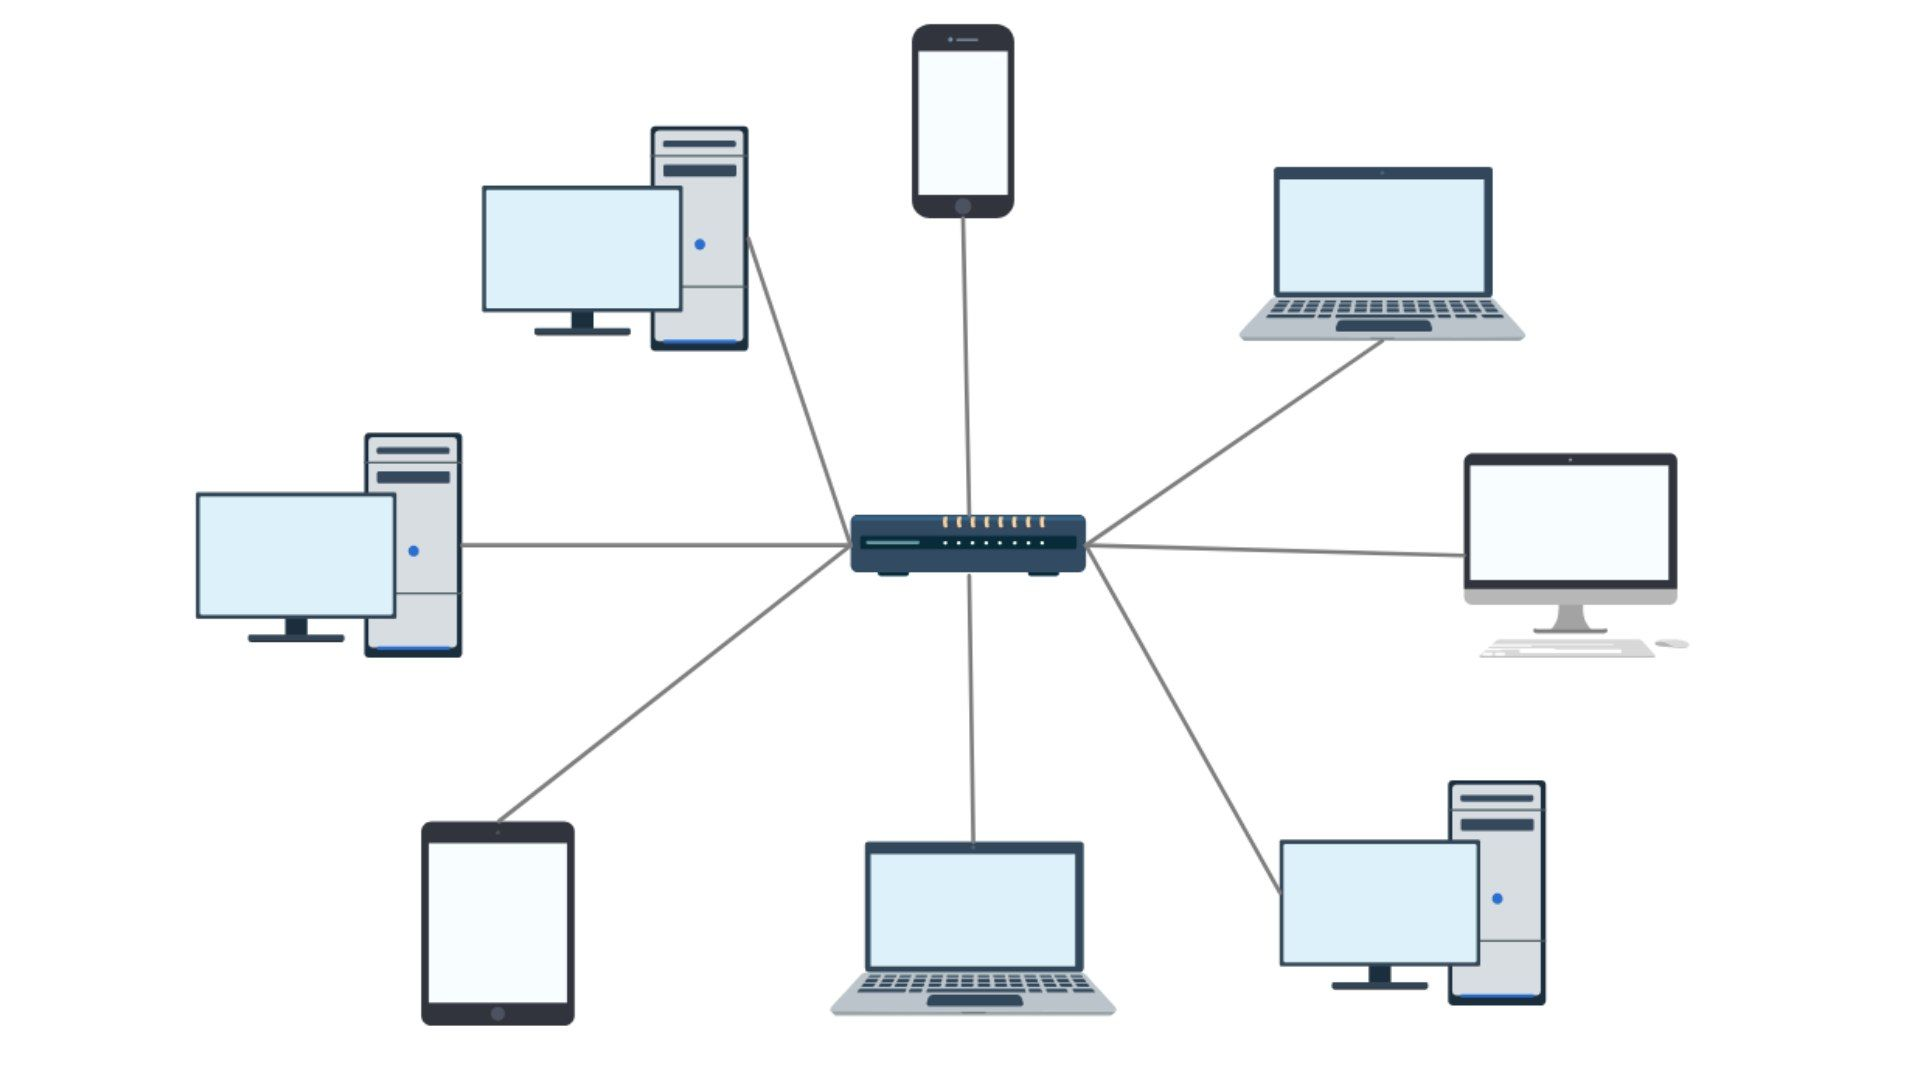
\includegraphics[width=0.6\linewidth]{figures/method/topo1.png}
    \caption[Structure of a generic Star Topology]{Structure of a generic Star Topology. Source: \cite{topo01}.}
    \label{fig:startopoGeneral}
\end{figure}

In a star topology, each node connects to a central instance, typically a hub or a switch. A generic star topology is shown in Figure \ref{fig:startopoGeneral}. The advantages of the star topology are simple installation beacuse of a linear hardware complexity (the number of required links is proportional to the number of nodes in the network) and high fault tolerance, as the network remains functional if a node fails. However, if the central instance fails, the network becomes non-functional.

Both topologies used are described in detail below. Any modifications made for specific test campaigns are indicated in the corresponding places in the thesis. This includes, for example, changes to the network interfaces used.

\subsection{Star Topology with a Switch in the Center} \label{chap:TopoSwitch}

\begin{figure}[h]
    \centering
    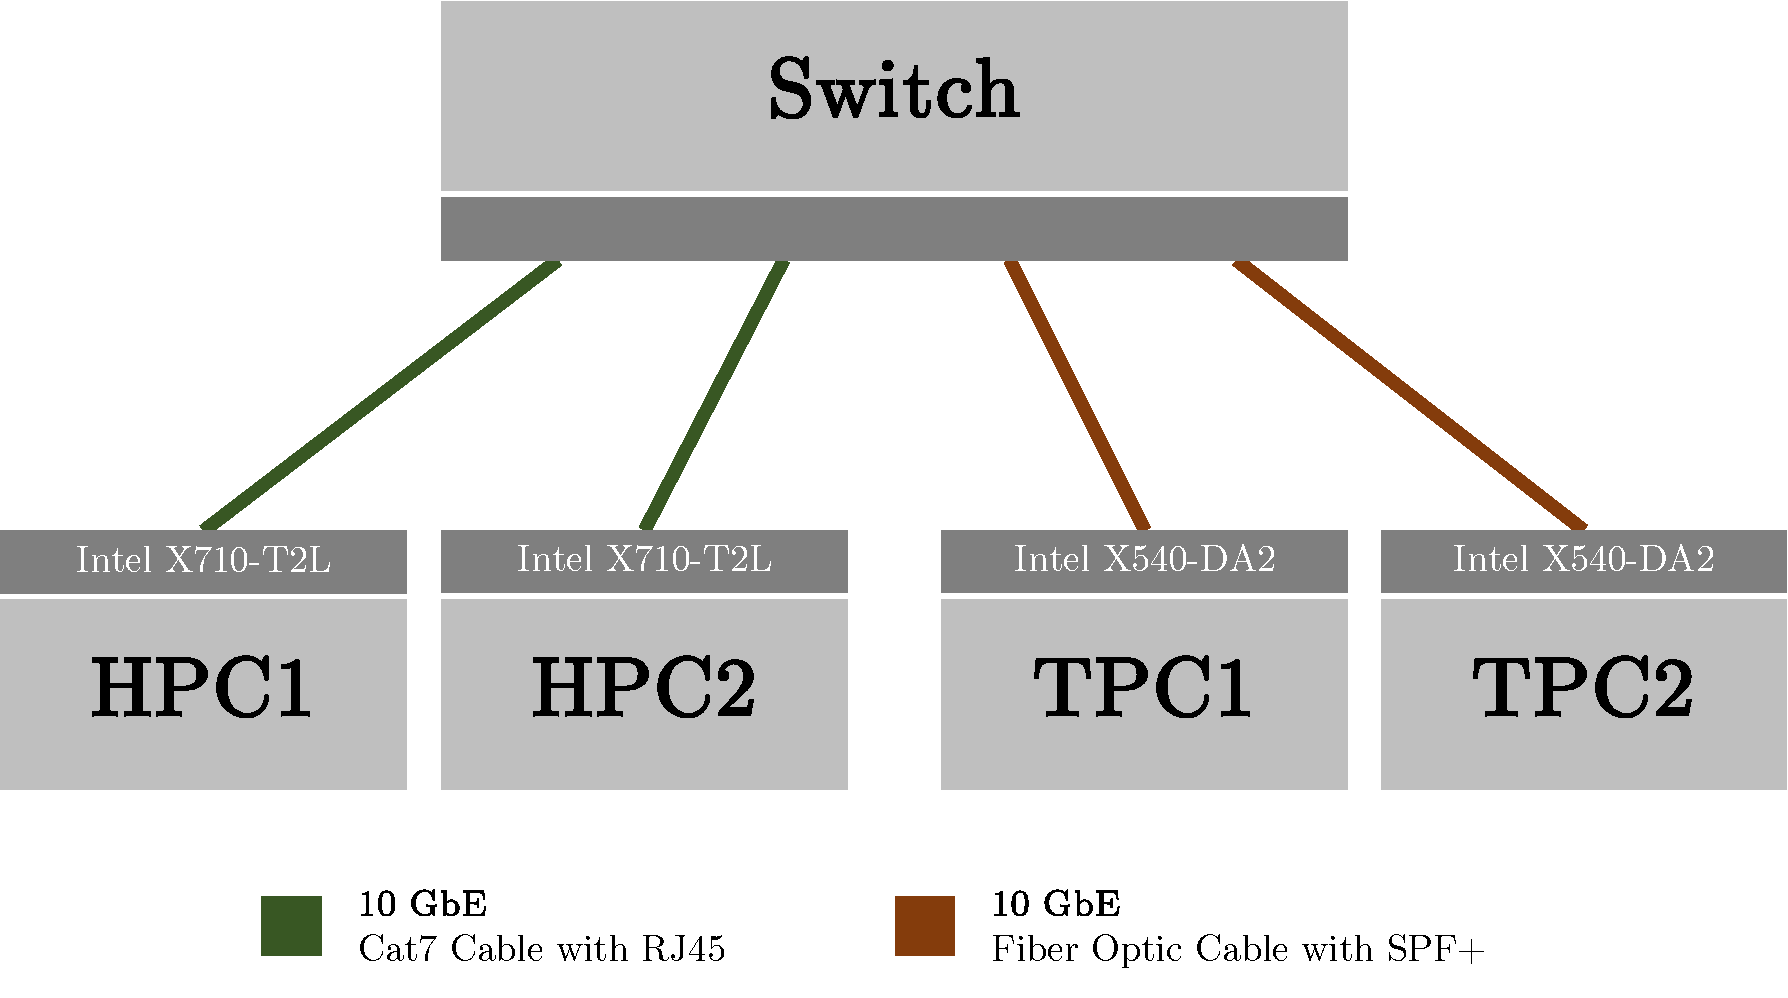
\includegraphics[width=1\linewidth]{figures/method/topo2.pdf}
    \caption[Visualization of the Star Topology with a Switch in the Center]{Visualization of the Star Topology with a Switch in the Center.}
    \label{fig:startopoSwitch}
\end{figure}

The first topology used is a star topology with a switch in the center, as shown in Figure \ref{fig:startopoSwitch}.

In this architecture, the Cisco CBS350-8XT switch, presented in \ref{chap:EthernetSwitch}, is located in the center of the star. All other participants, including two computer systems of type HPC and the computer systems of type TPC, are connected to this switch.

The HPC1 and HPC2 systems are both equipped with the Intel X710-T2L network card and are each connected to the switch with a bidirectional link using Cat7 copper cables. The TPC1 and TPC2 systems were equipped with the Intel X540-DA2 network card, which has SPF+ ports. They were connected to the switch via fiber optic cables using Intel SPF+ SR transceivers.

\subsection{Star Topology with the iHawk in the Center} \label{chap:TopoiHawk}

\begin{figure}[ht!]
    \centering
    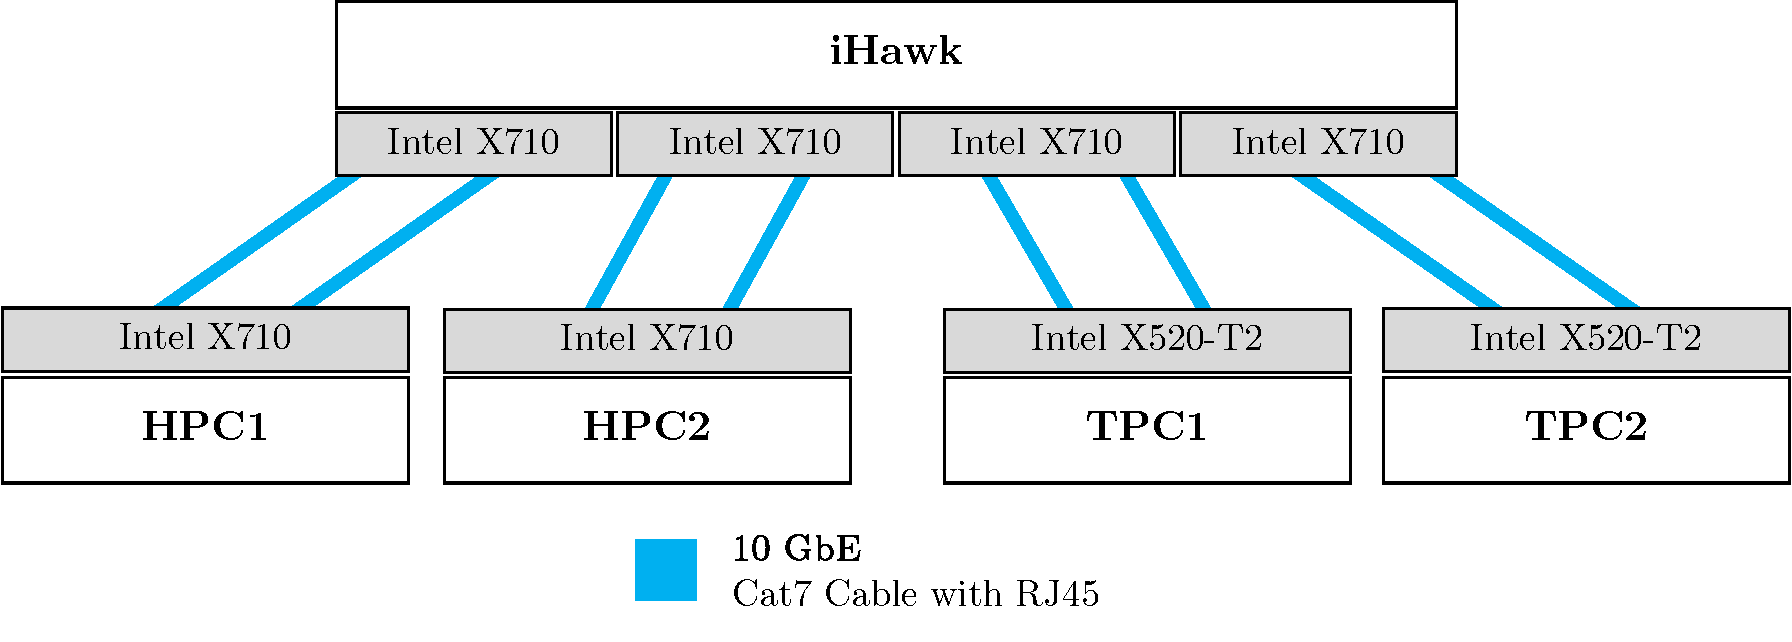
\includegraphics[width=1\linewidth]{figures/method/topo3.pdf}
    \caption[Visualization of the Star Topology with the iHawk in the Center]{Visualization of the Star Topology with the iHawk in the Center.}
    \label{fig:startopoIHawk}
\end{figure}

As the first topology presented proved to be unsuitable in the course of the tests carried out, a new topology as shown in Figure \ref{fig:startopoIHawk} was developed.

This new topology features an iHawk computer system at the center of the star, equipped with four Intel X710-T2L network interfaces. The HPC computer systems in this topology also have Intel X710-T2L network interfaces, while the TPC systems use Intel X520-T2 network interfaces. Each node is connected to the iHawk in the center via two bidirectional 10 GbE links.

\clearpage
\section{Introduction of the Test Program} \label{chap:TestSuite}
A dedicated test program, called TestSuite, was created to carry out the tests with the setup described above. The decision to create an own test program was based on the following considerations, which were not fully covered by existing network performance test programs such as iPerf \cite{testsuite01}:

\begin{itemize}
\item \textbf{Execution of tests with UDP protocol}: TestSuite focuses exclusively on tests with the UDP protocol and offers various setting options with regard to the generated and measured UDP communication. In addition to UDP sockets, Raw and Packet sockets are also supported.
\item \textbf{Results management}: TestSuite saves all relevant results of a test run in XML files, which facilitates subsequent evaluation.
\item \textbf{Focus on relevant aspects of the test}: The TestSuite places particular emphasis on testing packet loss and latency. This is reflected in various functionalities that stand out from existing test programs:

	\begin{itemize}
      \item Recording of losses with intermediate results throughout the test
      \item Recording of additional metrics for more precise investigation of packet losses
      \item Recording of send and receive timestamps for each packet
    \end{itemize}

\item \textbf{Automation of tests}: Due to the large number of tests that were expected in advance, the tests can be automated. This allows a more optimized utilization of the test setup to be achieved. Furthermore, required environmental conditions in the system, such as an additional system load, can be generated automatically.
\end{itemize}

Disadvantages of creating a custom test program is the additional time required for development and the presence of possible errors that could falsify the results. As the advantages listed above outweighed the disadvantages, the decision was made to develop the TestSuite.

This section first describes the software design of TestSuite. This is followed by a more detailed description of the communication generated and measured by TestSuite. Then, the interpretation and evaluation of the data generated during a test run will be considered and the relevant results recorded by TestSuite will be presented. The complete source code of the TestSuite can be found in the appendix.


\subsection{Software Design}
The TestSuite was developed using the C++ programming language in the C++20 version. The concept of object-oriented programming has been used. The Qt Creator IDE was used for programming. In the following, the concept of the TestSuite is explained before the architecture of the software is explained.

\subsubsection{Concept}

\begin{figure}[h!]
    \centering
    
\includegraphics[width=1\linewidth]{figures/method/swdesign1.pdf}
    \caption[Illustration of the TestSuite Concept]{Illustration of the TestSuite Concept.}
    \label{fig:tsconcept}
\end{figure}

The TestSuite is designed for reliability and performance testing with the topologies presented in \ref{chap:Architectures}. The basic concept of the TestSuite is shown in Figure \ref{fig:tsconcept}. TestSuite always generates and measures a UDP communication between a sender, also called a client, and a receiver, also called a server. The focus of TestSuite is on tests performed between two participants in a local network.

TestSuite is able to generate a UDP communication with a pre-defined payload and bandwidth and record associated metrics such as the number of lost packets or the latency between sending and receiving. The generated communication is a one-way communication, i.e. the server does not respond to messages from the client. One execution of TestSuite can generate and measure a maximum of one communication. If more than one communication is to be analyzed in a system, TestSuite can be executed multiple times.

\subsubsection{Architecture}

\begin{sidewaysfigure}
    \centering
    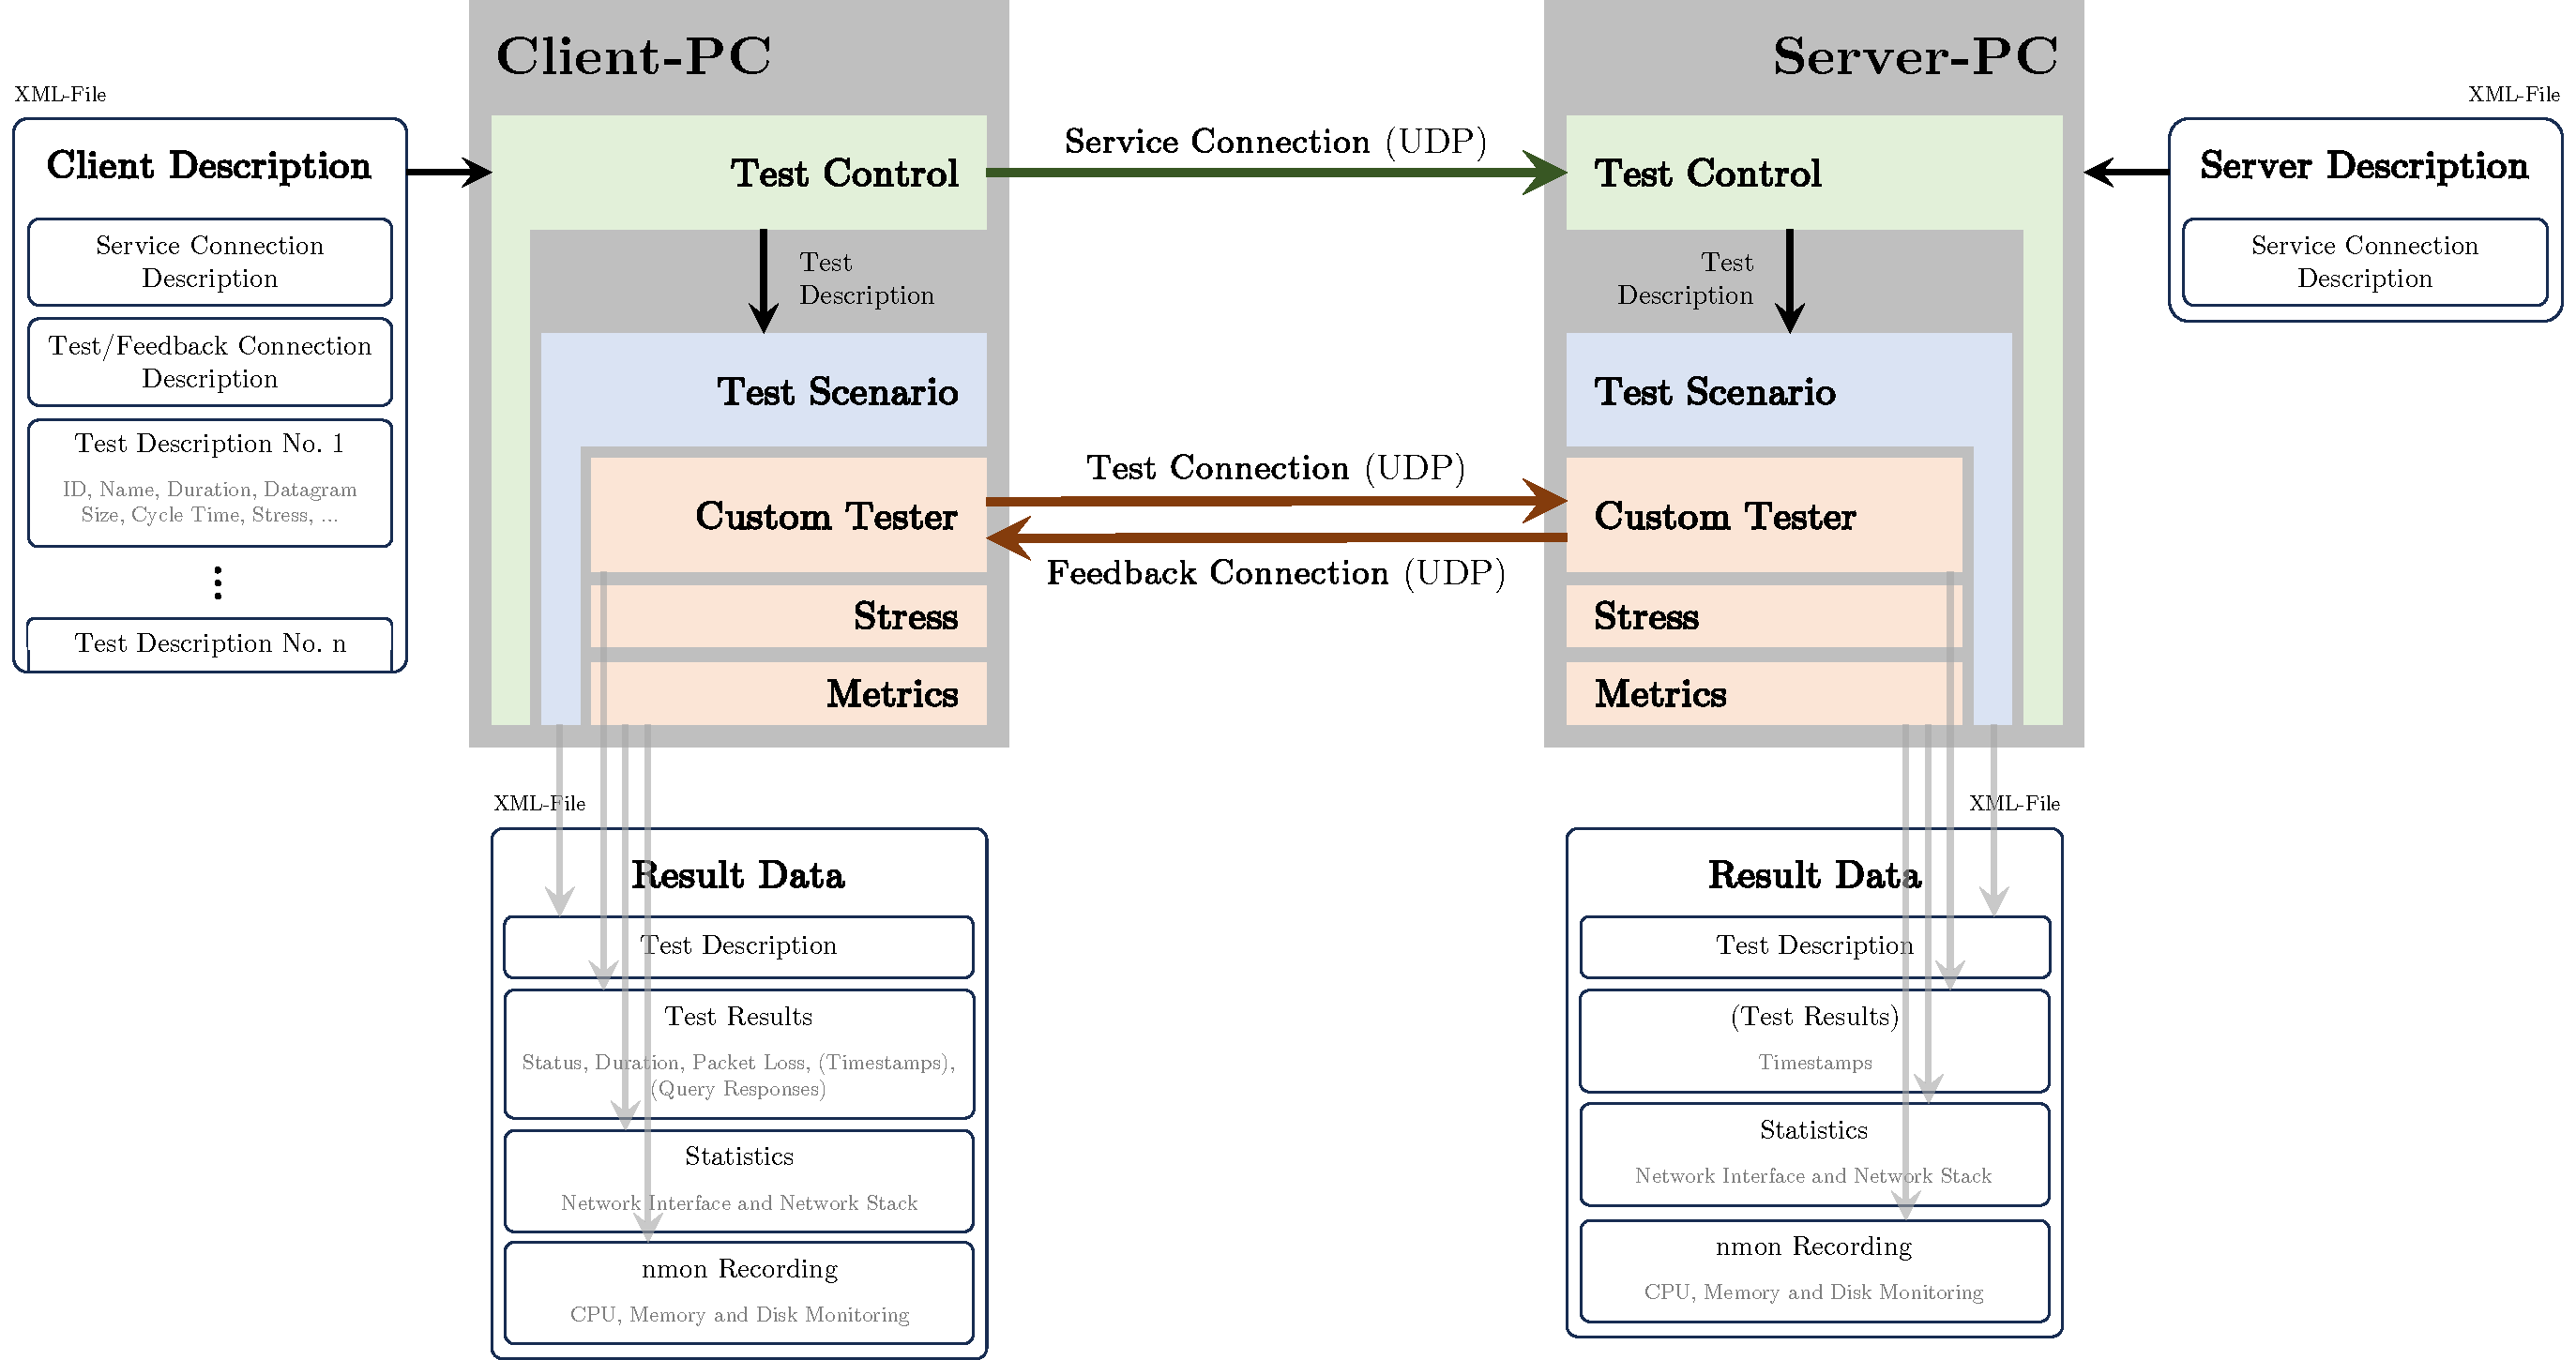
\includegraphics[width=1\linewidth]{figures/method/swdesign2.pdf}
    \caption[Architecture of the TestSuite with the relevant Classes, Data and Connections between the Systems]{Architecture of the TestSuite with the relevant Classes, Data and Connections between the Systems.}
    \label{fig:tsarch}
\end{sidewaysfigure}

Figure \ref{fig:tsarch} shows the architecture of TestSuite in a simplified form. The central elements are the systems on which TestSuite is executed. These are the client PC and the server PC. The client PC is also responsible for controlling the execution of the tests.

The input and output data is also shown. The diagram also shows the five central classes of the application and their hierarchy, as well as the various communication channels between the client PC and the server PC. The following sections describe these components in more detail.

\paragraph{Communication Channels}
Communication between the client PC and the server PC takes place via three separate communication channels, all using the UDP protocol.

The `Service Connection' is used to send configuration data to the server. This includes the description of the tests to be performed and the starting and stopping of a test execution. Furthermore, the configurations of the other communication channels, the `Test Connection' and the `Feedback Connection', are sent to the server.

The UDP protocol is used for the `Service Connection'. This is due to the fact that TestSuite focuses on tests between two participants in a local network, where packet loss is unlikely. However, UDP does not guarantee that the packets sent will reach their destination. Therefore, if TestSuite is to be used for tests over external networks in the future, a protocol should be used that guarantees the reliability of its transmission for this communication.

The `Test Connection' is the communication channel to be tested. A UDP communication is generated and measured according to certain parameters. This channel exists from the client to the server.

The `Feedback Connection' allows the server to send messages to the client during the current test run. This is also a UDP connection. The server sends the requested data only when requested by the client.

\paragraph{Input and Output Data}
All data required or created by TestSuite is written in Extensible Markup Language (XML). XML is a markup language for storing structured data in text form \cite{tsd01}. Because XML allows hierarchical storage of data and is human readable, it was used in TestSuite.

The pugixml library was used to read, process and create the XML files in TestSuite. pugixml is a C++ library that allows easy and efficient processing of XML files. More information about pugixml can be found in its documentation \cite{tsd02}.

In the following, the input data of the TestSuite, 'Client Description' and 'Server Description', as well as the output data will be examined in more detail.

\subparagraph{Input Data}
The TestSuite contains all inputs and configurations in the form of a `Client Description' or 'Server Description'. Both have a similar structure, but the Client Description is more comprehensive because the client is responsible for controlling the tests.

The first element present in both input files is a description of the `Service Connection'. This is used to exchange test management data between the systems. The description includes the server's IP address and port. This allows flexible variation of the port of the server, making it easy to run multiple independent TestSuites in parallel.

Next, the `Client Description' contains the configuration of the `Test Connection' and the `Feedback Connection'. This includes the IP addresses and port of both channels. In addition, the "Test Connection" description includes the names of the network interfaces used in the client and server, which are required to retrieve statistics. This communication channel also provides the option of using a Raw socket or a Packet socket in addition to a UDP socket.

The '`Client Description' also contains a description of the tests to be performed, the so-called 'Test Description'. The Client Description can contain any number of Test Descriptions, which are executed in sequence.

The `Test Description' is a central element of the TestSuite. It contains the complete description of a test execution and must be available in both the client and the server in order to run a test. The 'Test Description' includes:
\begin{itemize}
	\item \textbf{ID} and \textbf{name} of the test
	\item \textbf{Path} where the test results are stored
	\item \textbf{Duration} of the test
	\item Description of the communication to be generated with \textbf{datagram size} and \textbf{cycle time}
	\item Description of \textbf{stressors} for generating additional system load
	\item Configurations for \textbf{latency measurement} or the use of \textbf{query requests}
\end{itemize}

The data presented here is explained in more detail in \ref{chap:targetcom} This includes the configurations for generating communication, the generation of additional system load, latency measurement and query requests.

\subparagraph{Output Data}

Both the Client PC and the Server PC store their output data, called 'Result Data', in the form of XML files. The result data is re-generated for each test.

The first element of the 'Result Data' is the 'Test Description' of the test performed. This makes it easier to associate the output data with a specific test scenario and to analyze the results.

The output data also includes the test results. These vary depending on the test configuration, but typically include the following elements:
\begin{itemize}
	\item \textbf{Status} of the test execution (success or error)
	\item \textbf{Duration} of the test
	\item Number of packets \textbf{sent} and \textbf{received}, with intermediate results from the \textbf{query requests} if applicable
	\item \textbf{Timestamp} for the sending or receipt of each packet
\end{itemize}

The test results in the 'Result Data' for the server are less extensive. They usually only contain the timestamp for the arrival of each packet. The test results and their evaluation are discussed in more detail in Section \ref{chap:evaluationTS}.

The output data also contains statistics of the network interface or network stack in the respective system. These are recorded before the start and after the end of a test. The statistics are stored:
\begin{itemize}
	\item \textbf{Standard Interface Statistic} of used network interface: \\
	These statistics include the number of bytes and packets sent and received by the interface. They also include a counter for the number of packets dropped by the interface \cite{tsd03}.
	\item \textbf{Network Stack Statistic}: \\
	These statistics contain information about the protocol layer of the system. The information about UDP and IP is stored in the output data. This includes the number of packets sent and received by each protocol layer, as well as counters for dropped packets. The information about receive errors, such as insufficient buffer space, is particularly relevant for testing.
\end{itemize}

The output data also includes logs from the nmon tool. This is described in more detail in Section 2.3.X. The data includes minute-by-minute records of the system's CPU usage, memory usage, network interface data, and disk usage information.
% TODO

\paragraph{Classes}
TestSuite has 5 central classes, the functionality of which is briefly explained below.

\subparagraph{Test Control}
The `Test Control' class is responsible for controlling and automating the execution of the test campaign. For this purpose, the class processes the input data of the TestSuite, the `Client Description' or the `Server Description'.

An important task is to control the execution of the tests. This is done by the 'Test Control' on the client PC. The tests contained in the Client Description are executed sequentially by creating an instance of the Test Scenario class for each test.

In addition, `Test Control' in the client sends commands to start and stop a test and the 'Test Description' of the current test to the server via the `Service Connection'. The server is then able to execute the test accordingly.

\subparagraph{Test Scenario}
The `Test Scenario' class handles the overall management of a single test. To create an instance of the class, the `Test Description' of that test is required as a parameter.

The class will then create instances of the necessary components for that test according to the specifications in the 'Test Description'. This includes:
\begin{itemize}
	\item Class 'Custom Tester'
	\item Class 'Stress'
	\item Class 'Metrics'
\end{itemize}

\subparagraph{Custom Tester} \label{chap:customtester}
The `Custom Tester' class is responsible for generating and measuring the UDP communication and processing the test results. The generation and measurement of target communication as well as the associated configuration parameters and technical details are described in \ref{chap:targetcom}.

The data measured during a test is then processed and saved as an XML file. `Custom Tester' saves the "Test Results" section of the "Results Data" output data structure.

\subparagraph{Stress}
The `Stress' class is responsible for controlling the generation of additional system load during testing. This includes areas such as CPU load, I/O load, or network load.

The two programs `stress-ng' and `iPerf2' are used to generate these loads. These are described in more detail in Section \ref{chap:loadgeneration}. The `Stress' class of TestSuite controls these external programs, including starting, stopping, and configuring them.

The additional system load can be executed during a test on the client PC or the server PC, or on both systems simultaneously.

All configuration data for the additional system load is contained in the Test Description. This includes parameters such as the type of load, its intensity, or its location.

\subparagraph{Metrics}
The 'Metrics' class is responsible for collecting system metrics before, during, and after a test.

On the one hand, `Metrics' is responsible for recording the statistics of the network interface or the network stack in the systems before and after a test. The statistics are collected using the command line utilities 'ip' from 'iproute2' and 'netstat'. The output of these utilities is then processed using regular expressions, among other things, and important parameters are stored in the 'Statistics' section of the output data.

Another task of the `Metrics' class is to control the `nmon' program. `nmon' is a system monitoring tool for Linux operating systems. It monitors various system parameters such as CPU usage, memory usage, network traffic, disk activity, and other important system metrics \cite{tsd04}. Furthermore, nmon offers the possibility to record and store the system parameters cyclically.

The TestSuite creates an nmon recording for each test at runtime, in which the system parameters are recorded every 60 seconds. This recording is part of the 'Result Data'.

\subsection{Generation and Measurement of Target Communication} \label{chap:targetcom}
As explained in the description of the software design in \ref{chap:customtester}, the `Custom Tester' class is used to generate and measure the UDP communication.  In the following, this class will be introduced and the send and receive routines will be described in more detail.

\subsubsection{Parameters and Configuration Options}
A UDP communication is generated in the client part of the class and received by the server. Only a one-way communication is considered, i.e. the server does not send any messages other than those required to manage the test run. The generated UDP communication is characterized by the following parameters:

\begin{itemize}
	\item \textbf{Test Duration:} The test duration describes the maximum duration of the test and is specified in seconds.
	\item \textbf{Datagram Size:} As datagram size is referred to the size of the payload of the UDP segment in bytes.
	\item \textbf{Cycle Time:} The cycle time describes the minimum time between two calls of the send function of the socket. This is specified in nanoseconds and realized by a timer. With the cycle time, it is also possible to specify a target bandwidth.
\end{itemize}

\paragraph{Query} \label{chap:targetcom:query}
TestSuite has a query function which is part of the `Custom Tester' class and allows to determine the current number of packet losses during the test run.

The client sends a query to the server, which returns the number of packets received so far. The query is synchronized with the test, i.e. no more packets are sent until the response is received from the server. The query request is made after a pre-defined number of packets have been sent, which is defined with \texttt{QUERY\_FREQ}. In all tests performed, a query freqeuncy of 100,000 packets was selected.

The result of the queries, that is the total number of lost packets, is stored in a data structure. This is written to XML data after the test. This makes it possible to view the distribution of packet losses over the duration of the test. The query requests can also be used to abort the test prematurely. If a pre-defined threshold of lost packets, called \texttt{LOSS\_THRESHOLD}, is exceeded, the test is also terminated before the specified test duration has elapsed.

\paragraph{Timestamps} \label{chap:targetcom:timestamps}
The `Custom Tester' class also supports the recording of timestamps. The client records the time the packet was sent in the application, while the server records the time the packet was received in the application. Figure \ref{fig:TimestampLocation} displays the locations where the timestamps are recorded in relation to the perspective of the Linux network stack presented in \ref{chap:LinuxUDPNWStack}.

\begin{figure}[h!]
    \centering
    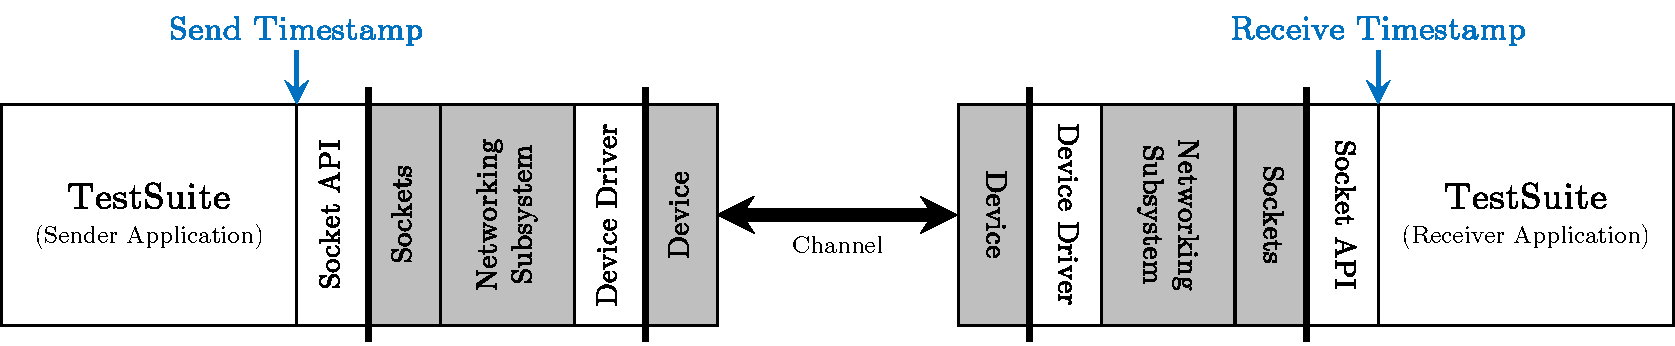
\includegraphics[width=1\linewidth]{figures/method/timestamps.pdf}
    \caption{Location of the Timestamp Recording in Relation to the Linux Network Stack.}
    \label{fig:TimestampLocation}
\end{figure}

The timestamps are stored on both systems in a data structure that is written to an XML file when the tests are complete. By calculating the difference between the time stamps, the latency between sending and receiving in the application can be determined. In order to calculate the latency using this method, synchronized clocks between the client and server are required. This synchronization is achieved in the test setup through the use of the Precision Time Protocol (PTP).

PTP, as defined in IEEE 1588-2008 \cite{perf01}, synchronizes distributed clocks in a network using the master-slave principle. The master sends messages with synchronization information, enabling all slaves to synchronize their internal clocks with the master. The protocol is also able to handle time delays introduced by the network.

\subsubsection{Implementation}
Selected features of the TestSuite implementation are described here. This includes the socket abstraction layer as well as the send and receive routine.

\paragraph{Sockets Abstraction Layer}
As mentioned above, the 'Custom Tester' generates a UDP communication. However, this can be generated not only with UDP sockets, but also with Raw and Packet sockets. To hide the differences in implementation and initialization of the individual socket types, the support class `uCE' was created, which hides the individual socket types from the 'Custom Tester' class.

The corresponding socket is initialized in the constructor of the `uCE' class, which requires the IP address of the client and server and a port number in addition to the socket type. This includes not only the actual creation of the sockets with the Socket API, but also the retrieval of additional information such as the MAC address of the network interfaces of the client and server using an ARP request.

The class provides the send and receive methods for sending and receiving UDP datagrams. Depending on the socket type used, the UDP, IP and Ethernet headers must be generated by the application before sending and removed after sending. This is also done by the class so that the application only receives the payload of the UDP message. For efficiency, no checksum is calculated when the headers are generated.

`uCE' also supports retrieving hardware timestamps from network interfaces to determine the time a packet was received or sent at the network interface. However, this is not supported by the network interfaces used in the test setup.

\paragraph{Send and Receive Routine}
\subparagraph{Send Routine}

\begin{lstlisting}[language=C++, caption=Simplified Code of the Send Routine., label=lst:sendcode]
int sequence_number = 0;
helpers_timer cycle_timer(CYCLE_TIME);

while(true) {
    if(current_time > end_time)
        break;

    sequence_number++;
    current_time = get_time();
    comm_client.send(TEST_MESSAGE, DATAGRAM_SIZE);

    if(QUERY_ENABLED && ((sequence_number % QUERY_FREQ) == 0)) {
        comm_client.send(QUERY_MESSAGE, sizeof(QUERY_MESSAGE));
          
        int received_counter = comm_server.receive();
        query_results.push_pack(sequence_number - received_counter);
        if((sequence_number - received_counter) > LOSS_THRESHOLD)
            break;
    }
  
    if (TIMESTAMPS_ENABLED) {
        timestamps.push_back(current_time);
    }

    timer_misses += cycle_timer.wait();
}

comm_client.send(STOP_MESSAGE, sizeof(STOP_MESSAGE));
int receive_counter = comm_server.receive();
\end{lstlisting}

Listing \ref{lst:sendcode} shows a simplified snippet of the send routine. The complete code can be found in the \texttt{run()} function of the \texttt{custom\_tester\_client} class in the appendix.

Initializations are done in lines 1 and 2. This includes a counter for the number of packets sent, called \texttt{sequence\_number}. In addition, the timer for realizing the cycle time is initialized.

The class \texttt{helpers\_timer} is used as the timer. This is also used in other projects in the context of the Test Support System. The timer implementation ensures a constant time interval between two calls of the \texttt{wait} method (see line 25) with the previously defined cycle time. If this interval has not expired, the timer in the \texttt{wait} method waits until the interval has expired. Otherwise, it returns immediately. The \texttt{wait} method returns the number of timer failures. This is equal to the number of missed time periods between this and the previous call to the method.

This ensures that the time between two calls of the \texttt{send} method (see line 10) is at least equal to the previously defined cycle time. It was decided to use the described timer instead of a normal sleep function with a fixed duration to achieve a constant interval between calls to the socket's send method. Since the send method of the Linux socket can block \cite{tsgen01}, this would not be possible using a sleep function, because the time required to call the \texttt{send} method would vary.

Before the start of each transmission loop, the system checks (see line 5) whether the previously specified test duration has been exceeded. If this is the case, the test is terminated. Then, before sending the UDP datagram, the current system time is retrieved from \texttt{CLOCK\_REALTIME}, the system-wide real-time clock under Linux \cite{tsgen02}, with a resolution in the nanosecond range (see line 9). This corresponds to the sending time of the datagram in the application.

In line 10 the UDP datagram is sent over the socket type specified in the 'Test Description'. Three different message types have been defined to differentiate the messages in the receiver. In addition to the \texttt{TEST\_MESSAGE} used here, there are also the \texttt{QUERY\_MESSAGE} and \texttt{STOP\_MESSAGE} types, which are described below. For messages of type \texttt{TEST\_MESSAGE}, the message contains an identifier that identifies the message and the current send counter. The rest of the payload of the UDP datagram is filled with random data to achieve the specified size.

Lines 12 through 19 contain the query request logic. As explained in \ref{chap:targetcom:query}, a request is sent synchronously to the server at a pre-defined frequency, and the server responds with its current receive counter. The difference between the send and receive counters corresponds to the current number of lost packets. This is stored in a data structure, namely a vector. If a pre-defined loss threshold is exceeded, the test is terminated prematurely.

In lines 21 to 23, if time stamps are enabled, the previously recorded time stamp is stored in a vector. In addition to the timestamp, the current sequence number is also recorded in order to assign the timestamps. For reasons of readability, this is not included in the simplified code snippet.

At the end of the test, regardless of whether this was triggered by exceeding the previously defined test duration or a loss threshold in connection with query requests, a stop message is sent (see line 28). This stops the receive routine in the server. The receive counter is then sent from the server. This can be used to determine the number of packet losses, which is stored in an XML file along with other metadata such as the exact duration of the test, the number of packets sent, the number of timer failures and, if applicable, the timestamps and results of query requests. This file is supplemented with additional metrics by other TestSuite classes.

\begin{table}[h]
\centering
\begin{tabular}{l|l}
	\toprule
	\textbf{Packet Size} & \textbf{Duration for a Loop Iteration} \\
	\midrule
	80 Byte & 6171 ns\\
	8900 Byte & 9726 ns\\
	65000 Byte & 63175 ns\\
	\bottomrule
\end{tabular}
\caption{Time for a single Iteration of the Transmission Loop for different Datagram Sizes.}
\label{tab:senditertime}
\end{table}

The table \ref{tab:senditertime} shows the time required for a single iteration of the transmission loop, averaged over 1000000 packets. To obtain the minimum times, the timer described above was not used. It can be seen that as the datagram size increases, the time for a loop pass increases. The reason for this is that as the datagram size increases, the duration of the call to the Linux API for sending with the corresponding socket increases, because more data has to be copied and processed in the kernel \cite{tsgen03}.

\subparagraph{Receive Routine}

\begin{lstlisting}[language=C++, caption=Simplified Code of the Receive Routine., label=lst:reccode]
int sequence_number = 0;

while(true) {
    message_type message = comm_client.receive();
    current_time = get_time();

    if(message == TEST_MESSAGE) {
        sequence_number++;

        if (TIMESTAMPS_ENABLED) {
            timestamps.push_back(current_time);
        }
    }
    else if(message == QUERY_MESSAGE) {
        comm_client.send(sequence_number, sizeof(sequence_number));
    }
    else if(message == STOP_MESSAGE) {
        comm_client.send(sequence_number, sizeof(sequence_number));
        break;
    }
}
\end{lstlisting}

Listing \ref{lst:reccode} shows a simplified snippet of the receive routine. The complete code can be found in the \texttt{run()} function of the \texttt{custom\_tester\_server} class in the appendix.

In the receive loop of the server (from line 3), the receive command of the class `uCE' is called at the beginning, which is blocking. This can be used to determine the message type, shown here in simplified form. Once a packet has been received, the current time is retrieved in the same way as in the send routine.

Then the different types of messages sent by the client are distinguished. If it is a normal test message (type \texttt{TEST\_MESSAGE}), the receive counter is incremented. If timestamp recording is enabled, the previously recorded receive time is stored in the vector. Again, the corresponding sequence number is recorded in the real implementation, analogous to the send routine.

If the message is a \texttt{QUERY\_MESSAGE}, the current receive counter is sent to the client. If the message is a \texttt{STOP\_MESSAGE}, the current receive counter is also sent. The send loop is then terminated.

At the end of the test, if enabled, the recorded timestamps are written to XML data. As with the client, these are supplemented with additional metrics for the server.


\subsection{Recorded and Analyzed Data} \label{chap:evaluationTS} 

The presentation of TestSuite has already dealt with the data provided by the program in several places. The following chapter will show how the relevant test results are determined from this data.
The most important data provided by the TestSuite are the counters for the number of packets sent and received, a measurement of the exact test duration and the time stamp for each packet. From these, the relevant metrics for reliability and performance testing can be determined.

To calculate the metrics presented below, a Phyton script called `eParser' has been created. This script reads the output data from the TestSuite and calculates the presented metrics and creates diagrams based on them. The script is included in the appendix.

\subsubsection{Packet Loss}
The counters for the sent and received packets can be used to determine the number of packet losses, as shown in equation \ref{eq:packetloss}. This calculation is already performed by the TestSuite.
In the context of the TestSuite and the evaluation of the results, the term "packet loss" is used. Strictly speaking, however, the TestSuite counts the UDP segments sent and received and the calculated number expresses the lost UDP segments.

\begin{equation}
Packet\ Loss = Sent\ Packets - Received\ Packets
\label{eq:packetloss}
\end{equation}

\subsubsection{Throughput}

Throughput is the amount of data transferred per unit of time and can be measured in bits per second. To define throughput, let's consider the example of Host A attempting to send a file to Host B. During the data transfer, two types of throughput can be measured: instantaneous throughput and average throughput. Instantaneous throughput is the rate (in Bits per second) at which Host B receives the file at a given time. Average throughput is defined as the number of bits divided by the number of seconds it took to complete the transmission \cite{datacalc01}. In the context of this thesis, the average throughput as calculated in equation \ref{eq:throughput} is always referred to.

\begin{equation}
Throughput = (Received\ Packets \cdot Datagram\ Size) / Duration
\label{eq:throughput}
\end{equation}

\subsubsection{Packet Rate}
The packet rate (see equation \ref{eq:packetrate}) represents the number of packets that are transmitted per unit of time. In contrast to throughput, the packet rate is not specified in bits per second but in packets per second. The average packet rate is considered in this paper.


\begin{equation}
Packet\ Rate = Number of Packets / Duration
\label{eq:packetrate}
\end{equation}

\subsubsection{Latency} \label{chap:LatencyExplanation}
Latency, often referred to as delay, is the amount of time it takes to transmit a message. Latency consists of the following 4 components (according to \cite{datacalc02}):

\begin{itemize}
	\item \textbf{Propagation Time:} time required for a signal to travel from the source to the receiver via the transmission path
	\item \textbf{Transmission Time:} time required to transmit all the data bits of a signal from the transmitter source to the receiver
	\item \textbf{Queuing Time:} time that data packets spend in a queue before they are sent
	\item \textbf{Processing Delay:} time required to process data at the sender or receiver
\end{itemize}

TestSuite considers the latency from sending a packet in the client application to receiving a packet in the server application. This can be calculated using the timestamps recorded by the client and server (see \ref{chap:targetcom:timestamps}). Thus, the latency can be determined for each transmitted packet as shown in equation \ref{eq:latency}.

\begin{equation}
Latency = Receive\ Timestamp - Send\ Timestamp
\label{eq:latency}
\end{equation}

When analyzing latency during a test run, two main values can be determined. The first is the \textbf{Worst Case Latency}, which reflects the maximum of all latency values recorded during a test. Additionally, the \textbf{Mean Latency} can be considered, which represents the average value of the recorded latencies during a test.

To determine the latency, synchronized clocks between transmitter and receiver are required. The accuracy of the measurement is largely determined by the quality of the clock synchronization.

\clearpage
\section{Generation of additional System Load} \label{chap:loadgeneration}
One requirement for the tests is that they should be possible under different operating conditions. Based on this requirement, the following categories of load were defined, which should be able to be produced in the test setup, either in isolation or together:
\begin{itemize}
	\item \textbf{CPU Load} \\
		In the area of CPU load, the system should be loaded in Linux user mode and kernel mode. The system load should also be generated by real-time processes.
	\item \textbf{Memory Load}
	\item \textbf{I/O Load} on the internal hard disk and thus on the PCIe links
	\item \textbf{Interrupt Load}
	\item \textbf{Network Load} and thus on the PCIe links
\end{itemize}

The existing tools stress-ng and iPerf2 were used to generate the defined load scenarios.

\subsection{stress-ng} 
Stress-ng is a  system stress testing tool designed to test various aspects of a computer system, such as CPU, memory and I/O, to their performance limits. It is used by system administrators, developers and testers to assess the stability and reliability of hardware and software under high load \cite{stress01}.

Providing over 270 different stress options, called stressors, in areas such as CPU load, memory allocation and access, and disk I/O, which can be used individually or in combination to create a realistic load scenario for a system \cite{stress02}. In addition, stress-ng provides options to control the duration and intensity of the stressors \cite{stress03}.

Stress-ng is a command line program that can also be called from other programs, such as TestSuite, using the \texttt{fork} \cite{stress04} and \texttt{execlp} \cite{stress05} commands.

In order to generate the additional system load in the CPU, memory, I/O and timer areas during a test, stress-ng was used as it is a proven tool for generating stress with easy control. The stressors used are briefly introduced and described below. A more detailed description of all stressors and options of stress-ng can be found in its manual \cite{stress03}.

\subsubsection{CPU Load} \label{chap:stressngCPU}
As per the requirements, the CPU load must be generated in both user space and kernel space for which different stressors have to be used. Additionally, section \ref{chap:loadgeneration} specifies the need to create a load through real-time processes.

\paragraph{Generation of CPU Load in User Space} \label{chap:CPUStressor}
To generate CPU load in the user space of the system, the stressor `cpu' from stress-ng is used. This stressor performs complex mathematical calculations, including integer and floating-point calculations, matrix operations, and checksum calculations, which place a heavy load on the CPU.

A worker of this stressor fully utilizes one CPU core. stress-ng provides an option for this particular stressor to limit the CPU load to an integer value between 0\% and 100\%. To fully utilize the system, stress-ng creates as many workers as the computer system has cores.

\begin{figure}[h!]
    \centering
    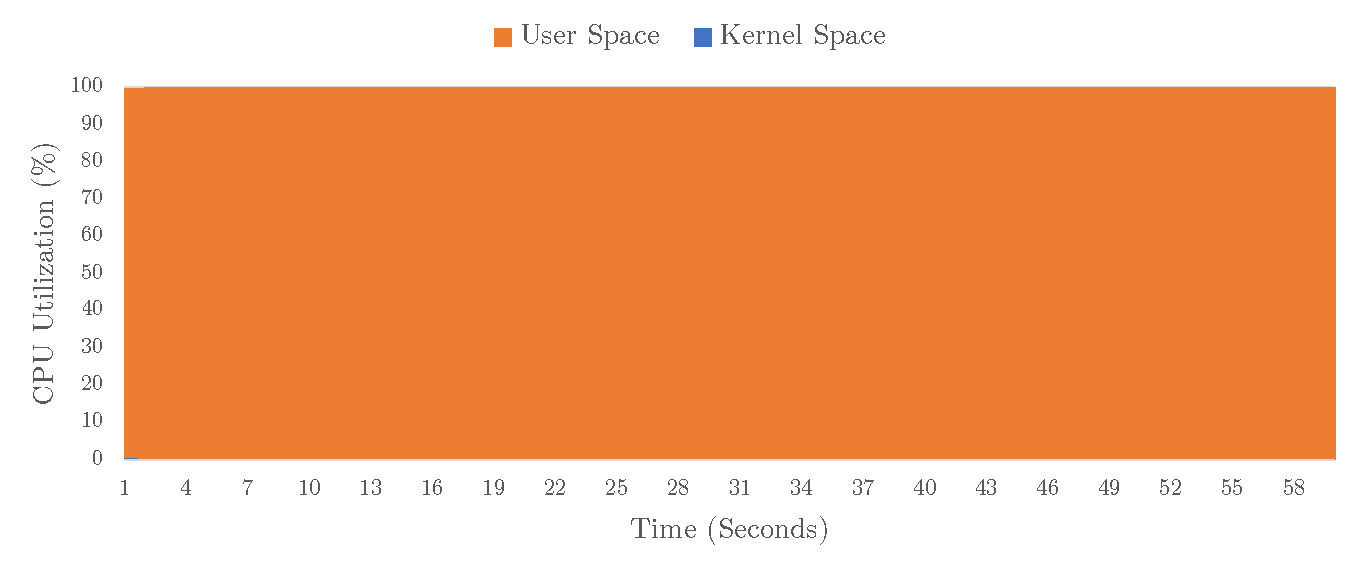
\includegraphics[width=1\linewidth]{figures/method/stress1.pdf}
    \caption{CPU Utilization during Execution of 16 stress-ng `cpu' stressors on HPC1.}
    \label{fig:stressCPU}
\end{figure}

Figure \ref{fig:stressCPU} displays the 1-minute execution of 16 `cpu' stressors on the HPC1 system, which has 16 logical CPU cores. It is evident that the `cpu' stressor fully utilizes this system. The load is generated in user space.

\paragraph{Generation of CPU Load in Kernel Space}
The `get' stressor is used to generate CPU load in kernel space. This calls various system calls, which leads to a predominant CPU load in kernel space. System calls such as \texttt{getpid} (retrieving the PID of the process \cite{stress06}), \texttt{getuid} (retrieving the user ID of the process \cite{stress07}) or \texttt{gettimeofday} (retrieving the current time \cite{stress08}) are used.

\begin{figure}[h!]
    \centering
    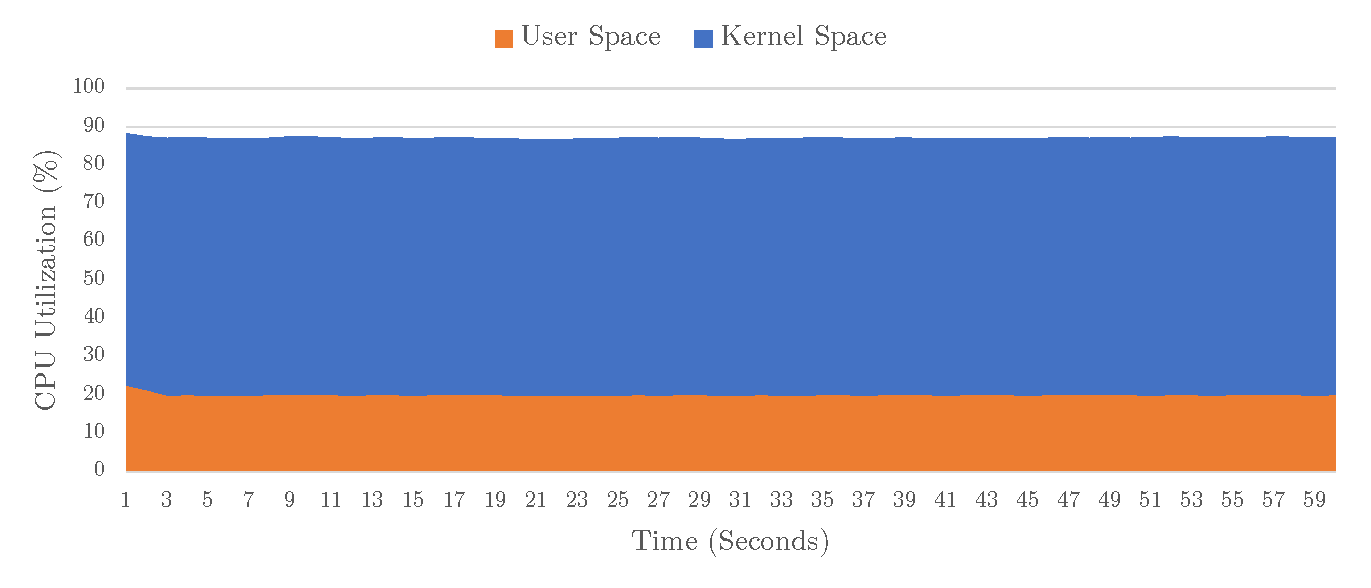
\includegraphics[width=1\linewidth]{figures/method/stress2.pdf}
    \caption{CPU Utilization during Execution of 16 stress-ng `get' stressors on HPC1.}
    \label{fig:stressGET}
\end{figure}

Figure \ref{fig:stressGET} displays the 1-minute execution of 16 `get' stressors on the HPC1 system. The stressor utilizes approximately 87.5\% of the total system load, with 20.1\% generated in user space and 67.4\% generated in kernel space.

As can be derived from Figure \ref{fig:stressGET}, this stressor does not fully utilize a CPU core. However, it still generates 60\% to 70\% of load in kernel space on a CPU core, making it suitable for generating CPU load in kernel space during tests.

\paragraph{Generation of CPU Load by Real-Time Processes}

stress-ng allows for the specification of a scheduling policy and priority as additional options. This allows each stressor to be executed as a real-time process. For generating load, the CPU stressor described in section \ref{chap:CPUStressor} was used with the \texttt{SCHED\_FIFO} scheduling policy described in section \ref{chap:RTProcess} and a scheduling priority of 50. The scheduling priority was intentionally set lower than that of the TestSuite because communication processes have a higher priority in the Distributed Test Support System.

\subsubsection{Memory Load} \label{chap:stressngMemeory}
To generate memory load, the stress-ng `bigheap' stressor is utilized. The stressor grows its heap by reallocating memory. In situations where low memory is available on the system, Linux employs an Out Of Memory (OOM) killer. This is a process executed by the kernel when the system runs out of memory that kills one or more processes to remedy this situation \cite{stress09}. If the process is killed by the Out Of Memory killer or if an allocation fails, the stressor will start again.

\begin{figure}[h!]
    \centering
    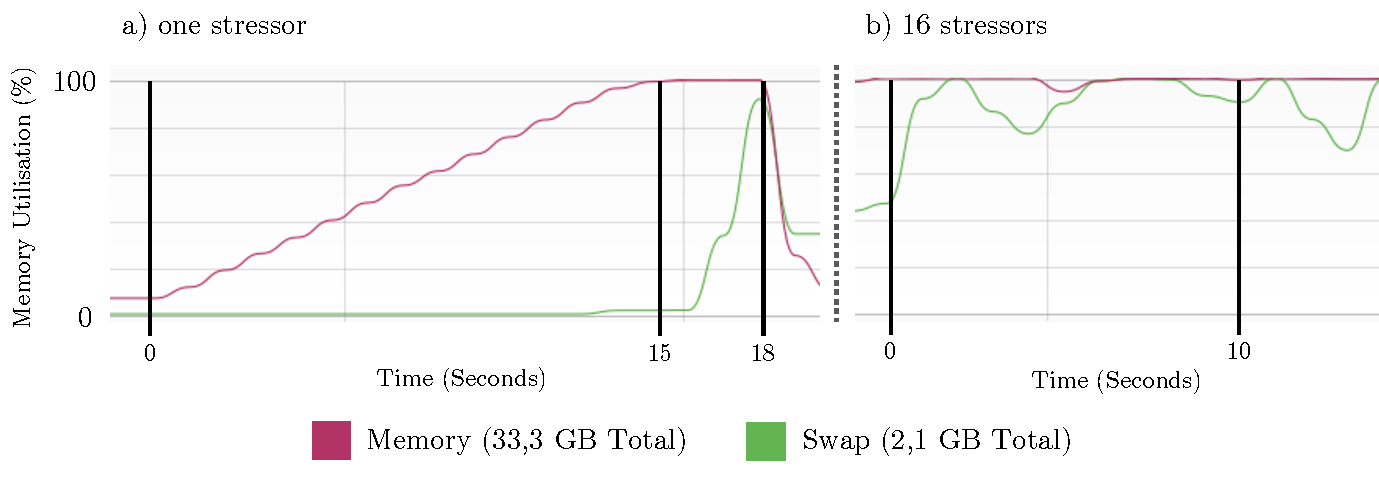
\includegraphics[width=1\linewidth]{figures/method/stress3.pdf}
    \caption{Memory Utilization during Execution of stress-ng `bigheap' stressors on HPC1.}
    \label{fig:stressMEM}
\end{figure}

Figure \ref{fig:stressMEM} displays the memory utilization over time for a `bigheap' stressor on HPC1 and compares it with the execution of 16 'bigheap' stressors that utilize all cores of the investigated computer system. The procedure for memory utilization is shown. The stressor requests more memory between 0 and 15 seconds until the memory is full, after which the system's swap increases. If the system has no more memory, the OOM killer terminates the process. The stressor is then restarted. If 16 'bigheap' stressors are executed simultaneously, this procedure overlaps.

The memory stressor, like any other process, also utilizes the system's CPU. Executing a memory stressor results in 100\% CPU utilization for one core.

\subsubsection{I/O Load} \label{chap:stressngIO}
The `hdd' stressor is used to generate I/O load. It performs continuous writes to the system's hard disk.

Figure \ref{fig:stressIO} shows the hard disk load for a 1-minute execution of an `hdd' stressor. It can be seen that this performs write operations at an average data rate of around 3.2 GBit/s. Furthermore, the data rate can fluctuate between 3 GBit/s and 3.8 GBit/s. The reasons for this is that the stressor works internally with different methods and iterates through them. The methods differ, for example, in the size of the files that are written to the hard disk. The execution of an hdd stressor leads to 100\% CPU utilization of a CPU core.

\begin{figure}[h!]
    \centering
    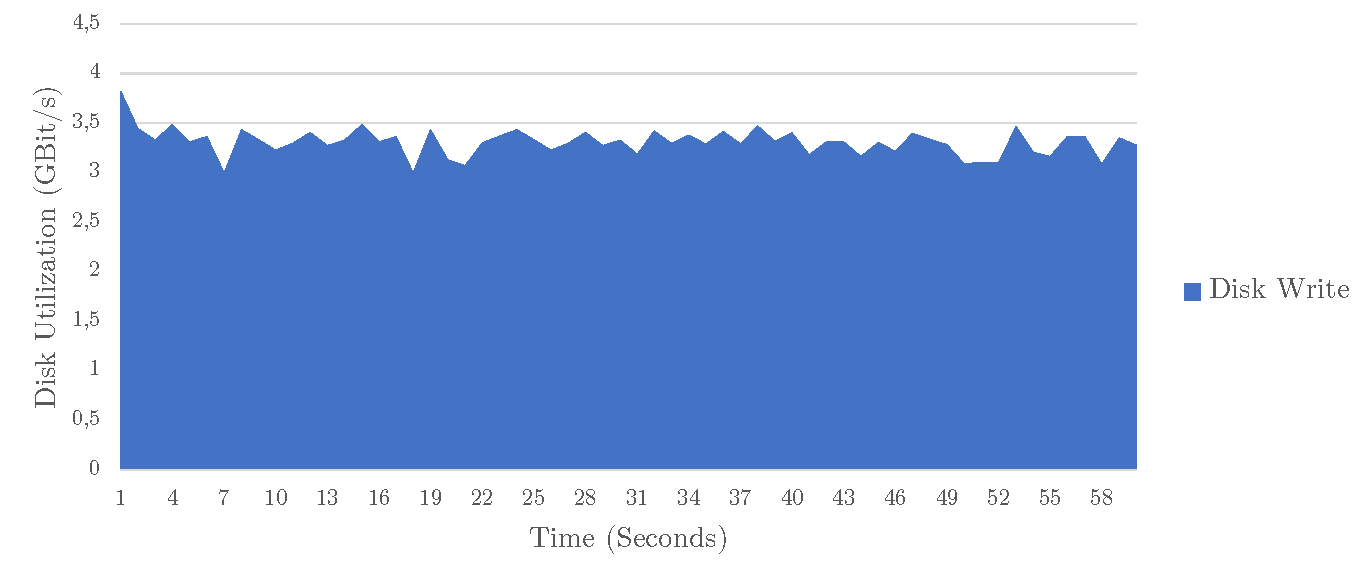
\includegraphics[width=1\linewidth]{figures/method/stress4.pdf}
    \caption{Disk Utilization during Execution of one stress-ng `hdd' stressors on HPC1.}
    \label{fig:stressIO}
\end{figure}

Linux has I/O scheduling, which reorders and groups requests based on the logical address of the data, with the goal of improving I/O throughput \cite{stress10}. To maximize I/O device stress, I/O scheduling was disabled by selecting the "none" scheduling policy.

stress-ng does not provide a default way to limit I/O stress by limiting the data rate. To achieve this limit, Control Groups (cgroup) were used. Control groups are a kernel function that can limit the resource utilization of processes. In some tests in this work, control groups were used to limit the maximum data rate of the HDD stressor. Further information on the used cgroup2 can be found in its documentation \cite{stress11}.

\subsubsection{Interrupt Load} \label{chap:stressngInterrupt}
The `timer' stressor was utilized to generate load in the domain of interrupts. This produces timer events at a rate of 1 MHz, resulting in timer clock interrupts. Each timer event is then intercepted by a signal handler. The purpose of this stressor is to test the system under high interrupt load \cite{stress02}. The execution of one timer stressor also fully utilizes a CPU core to 100\%. Additionally, the system is loaded by the processing of the signal handler. The entire system's utilization was examined using an HPC as an example, which amounts to approximately 6.3\%.

It is important to note that the timer results generated in this manner differ from interrupts generated by external hardware. Although both events are asynchronous \cite{like02}, there is a significant difference between them. Timer events are generated periodically by the operating system, while hardware interrupts are triggered unpredictably by external devices such as network devices \cite{stress14}. Signal handlers execute timer events in the context of the respective process, while interrupt handlers process hardware interrupts directly in the kernel \cite{like02}.




\subsection{iPerf2}
iPerf2 is a tool for measuring bandwidth between two hosts on IP networks. It works according to the client-server principle, where the client is the sender and the server is the receiver. iPerf supports protocols such as TCP and UDP.

Various parameters can be specified when performing a measurement. These include the test duration, the datagram size or a target bandwidth. At the end of each measurement, iPerf reports the achieved bandwidth, jitter and packet losses. More information about iPerf can be found in its documentation \cite{testsuite01}.

In this work, iPerf is used with the UDP protocol for a given target and datagram size. The only goal is to generate network traffic. To measure reliability and performance characteristics, only the TestSuite presented in Section 3.3 is used as part of the thesis.
    \chapter{Analysis of Reliability}

\section{Test Objectives}

The test campaigns presented here aim to investigate the reliability of UDP communication using an UDP socket in a local network under conditions similar to those in the Distributed Test Support System. Reliability is measured by the number of lost packets. Both topologies presented in \ref{chap:Architectures} were considered.

The investigation can be considered successful if no packet loss occurs in the test setup under all operating conditions.

Packet loss can occur at several points within the network. On the one hand, it can be caused by a participating computer system. Possible causes include an overflow of the socket receive buffer or the network interface buffer (RX\_Ring or TX\_Ring). The QDisc queue, which is used in the network stack to send packets, can also overflow. In addition, limited system resources, such as CPU and memory contention or high interrupt handling, can also lead to packet loss.

In the tests using the star topology with a switch in the centre (see \ref{chap:TopoSwitch}), packet loss may also occur due to this switch. Possible reasons for this are exceeding the maximum switch capacity, which is 160 GBit/s, or an egress buffer overflow. These buffers have a size of 6 MB, and are dynamically shared between all ports \cite{setup09}.

\clearpage
\section{Reliability Analysis of the Star Topology with a Switch in the Center} \label{chap:switchtest}

\subsection{System under Test}
The test campaigns presented in this chapter utilize the star topology with a switch in the center (see \ref{chap:TopoSwitch}). All systems are connected to each other through the Cisco CBS350-8XT switch. The network interfaces mentioned in the architecture presentation are utilized in the computer systems.

\begin{figure}[h!]
    \centering
    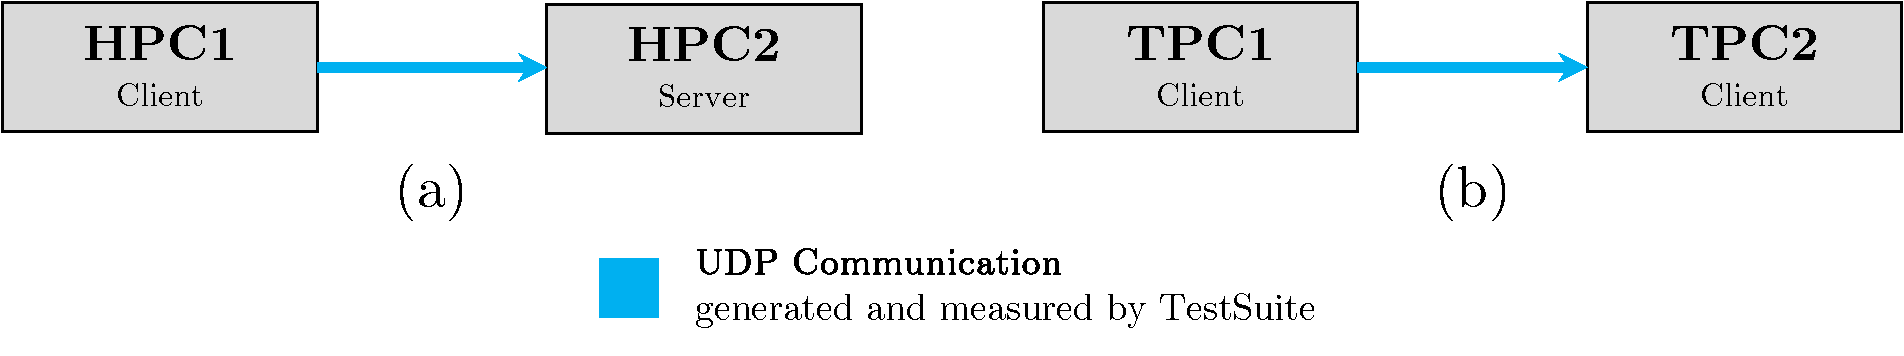
\includegraphics[width=1\linewidth]{figures/reliability/star/rel_g_1.pdf}
    \caption{Illustration of the used Systems under Test.}
    \label{fig:sutreliability}
\end{figure}

One system under test is a UDP communication generated by the Test Suite between the two High-Performance PCs (see Figure \ref{fig:sutreliability}a). HPC1, is the sender, also referred to as the client, and HPC2 is the receiver, also referred to as the server. Additionally, tests were conducted using the two Traffic PCs as the system under test (refer to Figure \ref{fig:sutreliability}b). The default settings of the network interfaces were used for all tests.

\subsection{Test Campaings}

\subsubsection{Isolated Tests in Different Operating States} \label{chap:relcamp1}
\paragraph{Motivation and Context}

As mentioned above, certain operating conditions can cause packet loss due to limited system resources. The purpose of this campaign is to identify the type of load on the test setup that causes packet loss. The following operating states are considered:

\begin{itemize}
  \item \textbf{System without any additional Load}
  \item \textbf{CPU Load} in User Space, Kernel Space and by Real-Time Processes (see \ref{chap:stressngCPU})
  \item \textbf{Memory Load} (see \ref{chap:stressngMemeory})
  \item \textbf{I/O Load} on internal Hard Disk (see \ref{chap:stressngIO})
  \item \textbf{Load due to Timer Interrupts} (see \ref{chap:stressngInterrupt})
  \item \textbf{Network Load} \\
  		Additional network load was generated with a participating computer system of the system under test. In the example of the High-Performance PCs as the SuT, this means UDP communication between the client or server and a Traffic PC. The Traffic PC is acting as the sender, and the respective computer system of the SuT is acting as the receiver.
  		
  \item \textbf{Traffic Load} \\
 		Traffic Load refers to bi-directional UDP communication between computer systems that are not part of the current system under test. The objective is to strain the switch.
\end{itemize}

The tools presented in \ref{chap:loadgeneration} are used to generate this load. The system is tested under maximum load. This means that as many stressors are used for the load generated with stress-ng as the system has logical CPU cores. A bandwidth of 10 GBit/s is used for the network stressors.

The presented operating states were tested individually for client and server. The two Traffic PCs as well as the High-Performance PCs were used as the system under test. The test duration for all tests was 100 seconds and a cycle time of 0 µs was used, whereby the maximum possible bandwidth was used for transmission. The datagram sizes used were 80 bytes as a representative for small datagrams in the test support system, 8900 bytes as a datagram size close to the MTU, and 65000 bytes as a datagram size close to the maximum of UDP.

\paragraph{Results}
In tests where the client was subjected to a generated load, no packet loss was detected in any of the tested operating states. This applies to both the tests with High-Performance PCs and Traffic PCs as a system under test.

\begin{figure}[h!]
  \centering
  \subcaptionbox{High-Performance PCs as System under Test\label{fig:resuc1a}}{%
    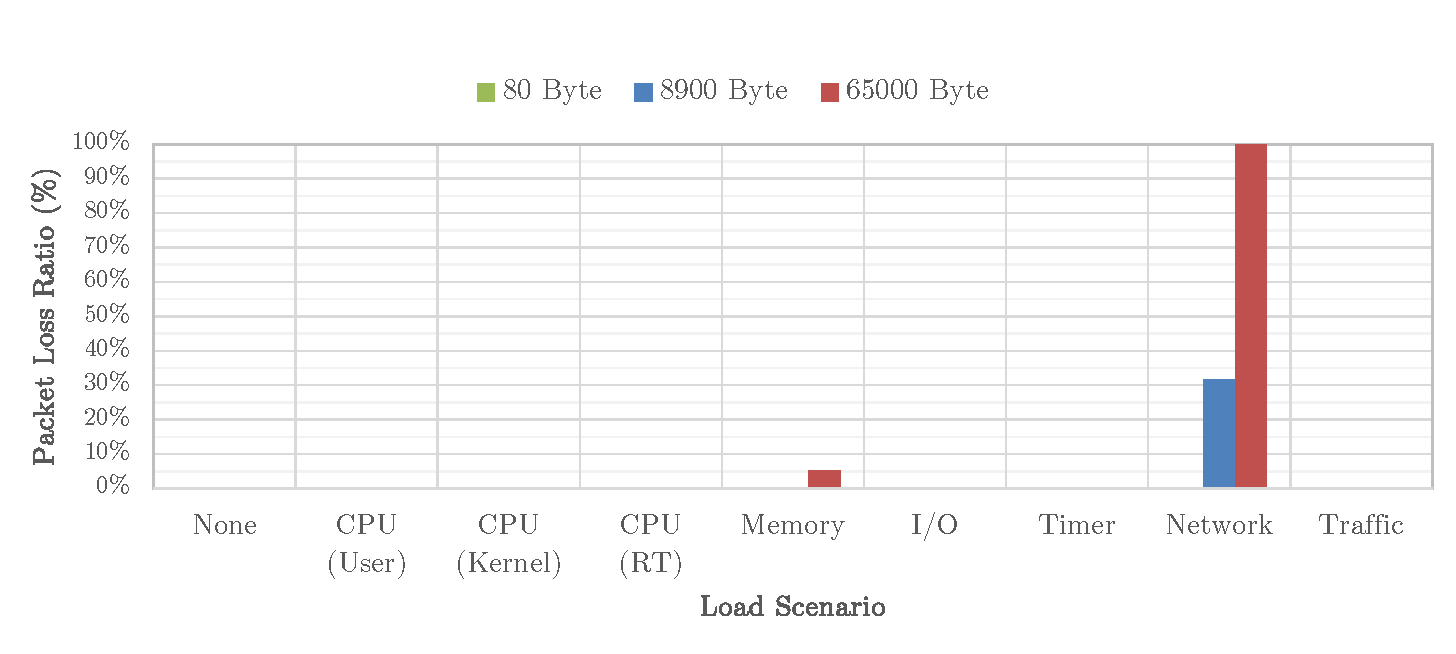
\includegraphics[width=1\textwidth]{figures/reliability/star/rel_d_1a.pdf}
  }
  \subcaptionbox{Traffic PCs as System under Test\label{fig:resuc1b}}{%
    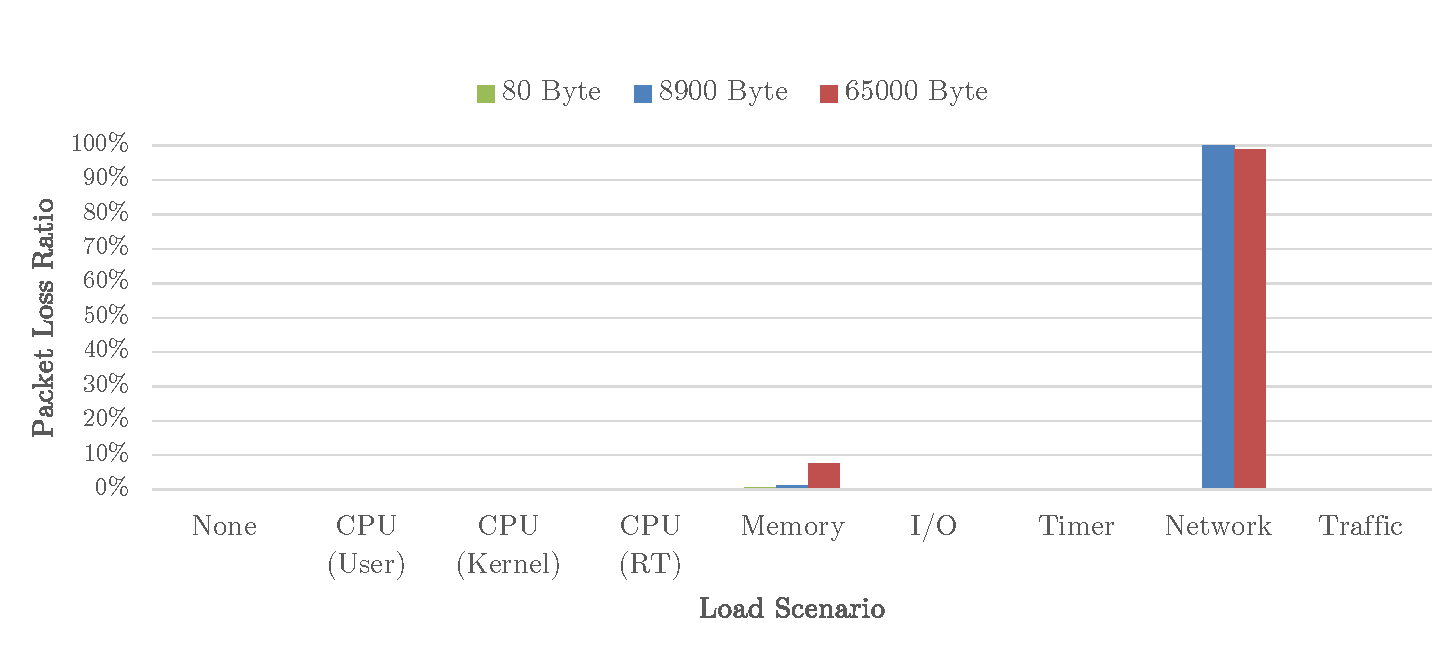
\includegraphics[width=1\textwidth]{figures/reliability/star/rel_d_1b.pdf}
  }
  \caption{Packet Loss Ratio for various Load Scenarios with different Datagram Sizes (Campaign `Isolated Tests in Different Operating States').}
  \label{fig:resuc1}
\end{figure}

During the stress tests where the server was subjected to a generated load, packet losses occurred on both systems under test. Figure \ref{fig:resuc1a} displays the percentage of packet losses in different load scenarios for High-Performance PCs, while Figure \label{fig:resuc1b} shows the results for Traffic PCs. The diagrams demonstrate that packet losses occurred in both systems under test when subjected to the stress-ng 'bigheap' stressor which generates memory load and to network load on the server.

Under stress from memory load, the server experiences packet losses across all three datagram sizes tested. Losses are less than one percent for 80 bytes and 8900 bytes, which is why they are not visible on the diagram. However, they increase to 5.29\% and 7.81\% for 65000 bytes, which is due to fragmentation, since the entire datagram is lost when a fragment is lost. It is also observed that the losses are slightly lower with the High-Performance PC as the system under test compared to the Traffic PC as the system under test when under memory load.

The losses occurred in the server, and the network card dropped the packets, as determined by the standard interface statistics of the network interface in the server. The drops occur due to memory load, as explained in \ref{chap:stressngMemeory}. This results in insufficient memory to process the arriving packets through the network stack. For instance, the network stack may not be able to allocate a socket buffer structure to process an incoming packet.

Additionally, packet losses have been observed with network load for datagram sizes of 8900 bytes and 65000 bytes. These are due to the maximum bandwidth being exceeded because both the client and another computer system are sending data to the server at up to 10 Gbit/s. As a result, the maximum bandwidth of 10 GBit/s, with which the server is connected to the switch, is exceeded, which is why packets get dropped by the switch.

\begin{figure}[htbp]
  \centering
  \subcaptionbox{Datagram Size of 80 Byte\label{fig:resuc2a}}{%
    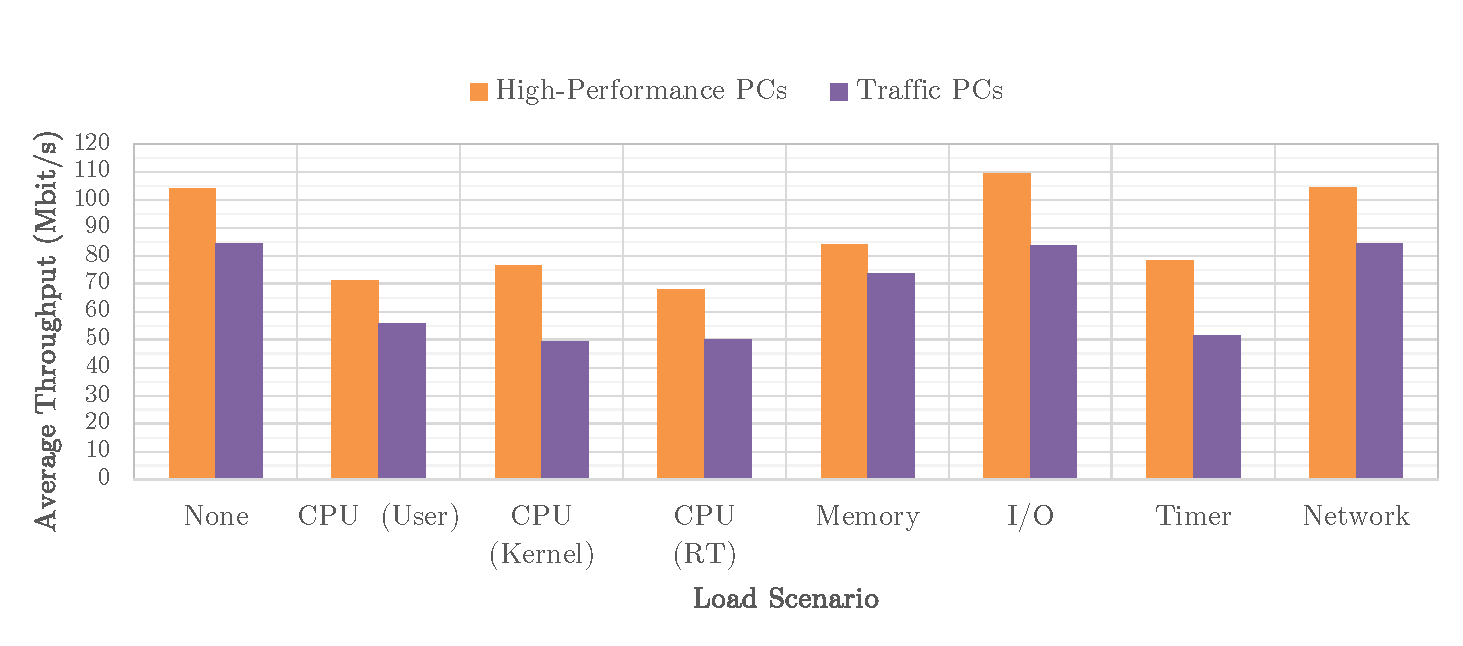
\includegraphics[width=0.9\textwidth]{figures/reliability/star/rel_d_2a.pdf}
  }
  \subcaptionbox{Datagram Size of 8900 Byte\label{fig:resuc2b}}{%
    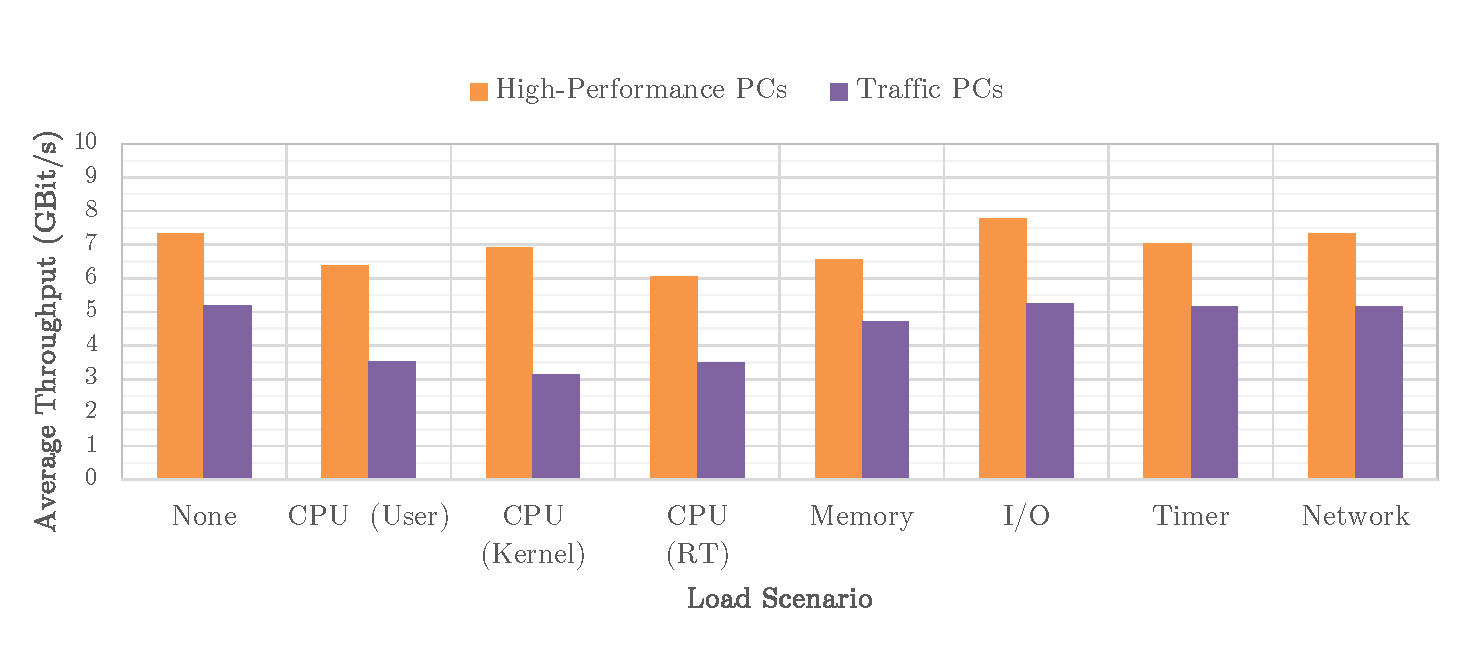
\includegraphics[width=0.9\textwidth]{figures/reliability/star/rel_d_2b.pdf}
  }
    \subcaptionbox{Datagram Size of 65000 Byte\label{fig:resuc2c}}{%
    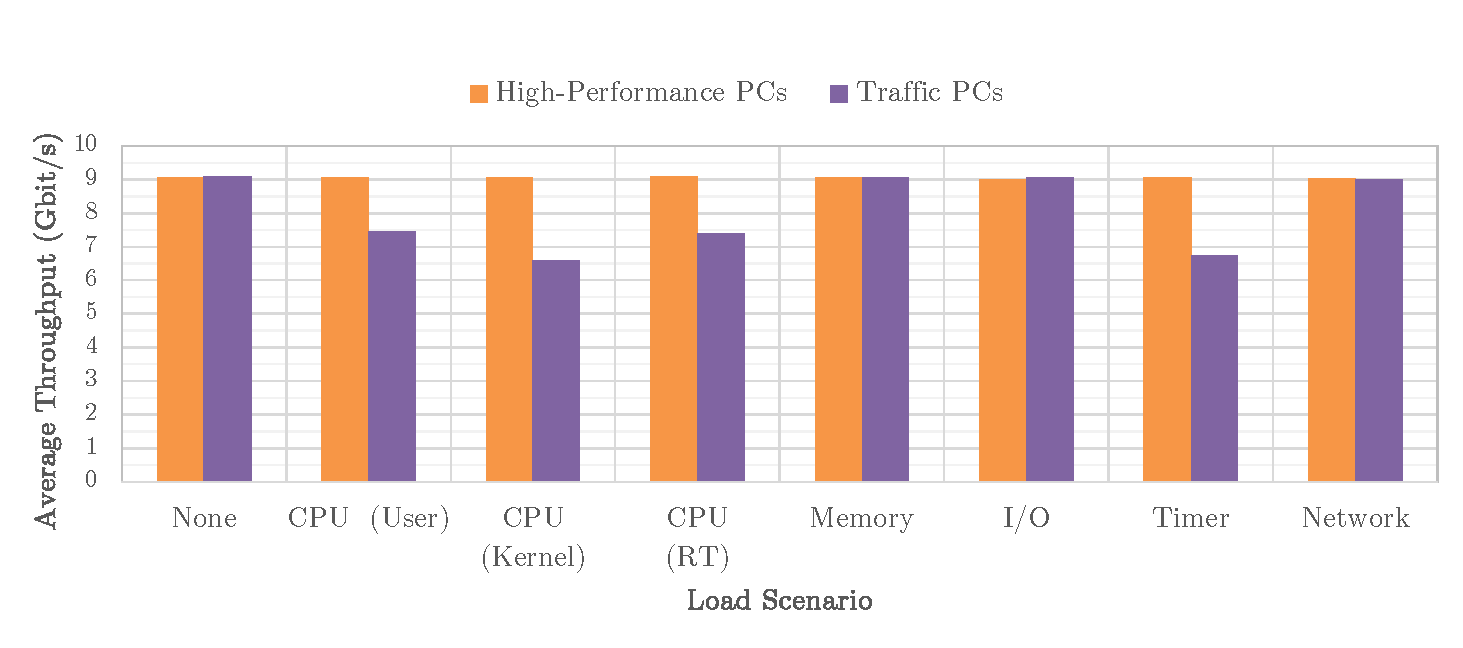
\includegraphics[width=0.9\textwidth]{figures/reliability/star/rel_d_2c.pdf}
  }
  \caption{Average Throughput for various Load Scenarios (Campaign `Isolated Tests in Different Operating States').}
  \label{fig:resuc2}
\end{figure}

As mentioned above, there were no packet losses during the tests where the client was loaded. However, the stress did affect the average throughput sent to the server. Figure \ref{fig:resuc2} compares the average throughput of the High-Performance PCs and Traffic PCs as system under test in different operating conditions.

On one side, the average throughput of the High-Performance PCs is higher than that of the Traffic PCs, especially for datagram sizes of 80 bytes and 8900 bytes. All categories of CPU load, memory load, and load due to timer interrupts have a negative impact on the average throughput, with a reduction of 5\% to 10\% greater for Traffic PCs than for High-Performance PCs, particularly for datagram sizes of 80 bytes and 8900 bytes.  At 65,000 bytes, the throughput of High-Performance PCs remains unaffected by any stress, while the throughput of Traffic PCs is reduced by up to 25\% by CPU and timer interrupt load.

These differences in average throughput and the impact of additional system load on it are due to differences in hardware. The hardware of High-Performance PCs is significantly more powerful than that of Traffic PCs (see \ref{chap:ComputerHardware}), which enables them to transmit a larger number of packets.

\paragraph{Classification of Results}
The campaign found that the reliability of the server can be negatively impacted by the memory load and network load operating states. However, it is important to note that these isolated operating conditions are not realistic.

A system that constantly suffers from a memory overload, as caused by the memory load scenario, is a conceptual error because too less memory is installed.

Regarding the examined network load scenario, it is logical to discard packets if the maximum bandwidth is exceeded. However, it should be noted that this situation can occur in asynchronous systems, such as a Distributed Test Support System.

\subsubsection{Tests with Realistic Load Scenario} \label{chap:campaignloadscen}
\paragraph{Motivation and Context}
In the previous campaign (refer to \ref{chap:relcamp1}), individual operating states were considered in isolation. The highest possible load was always taken into account, but this does not correspond to the typical load in a Distributed Test Support System.

{
\renewcommand{\arraystretch}{1.3}

\begin{table}[h]
\centering
\newcolumntype{C}[1]{>{\raggedright\arraybackslash}p{#1}}

\begin{tabularx}{\textwidth}{C{8cm} | l | X}
	\toprule
	\textbf{Load Component} & \textbf{Quantity} & \textbf{Analogy}\\
	\midrule
	Real-Time Process with 100\% CPU Utilization & 4 & Simulations\\
	Real-Time Process with 5\% CPU Utilization & 20 & Global Memories\\
	Process with I/O Load on internal Disk with Data Rate limited to 1 GBit/s & 1 & Data Logging\\
	Timer with a Frequency of 100 kHz & 1 & \\
	\bottomrule
\end{tabularx}

\caption{Components of the Realistic Load Scenario for a Computer System.}
\label{tab:realpc}
\end{table}
}

\vspace{20pt}

\begin{figure}[h!]
    \centering
    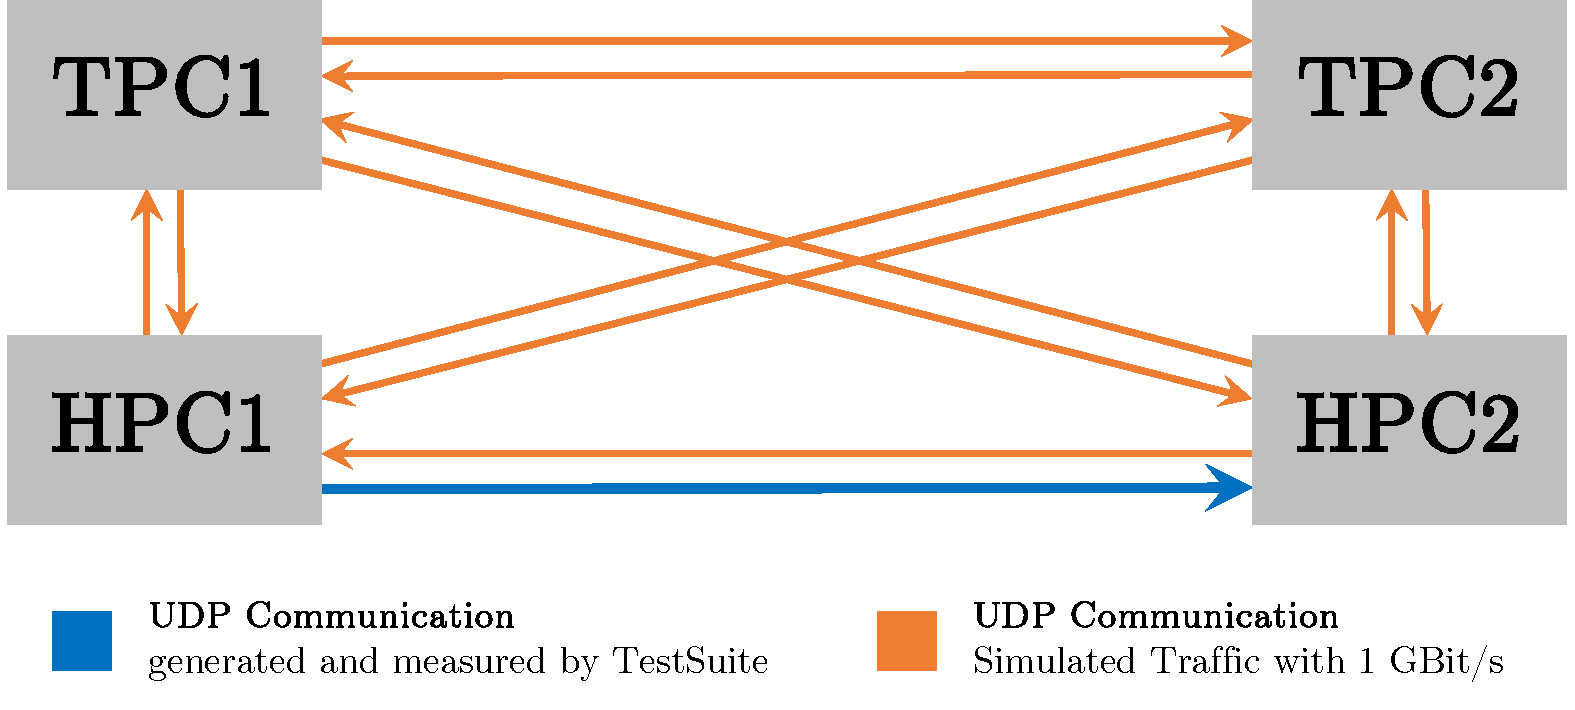
\includegraphics[width=0.8\linewidth]{figures/reliability/star/rel_g_2.pdf}
    \caption{Representation of the Network Load in the Realistic Load Scenario.}
    \label{fig:realNW}
\end{figure}

Therefore, a realistic load scenario has been developed based on practical experience with a Distributed Test Support System, which includes the load on the computer systems as well as on the network. Table \ref{tab:realpc} contains the components of this scenario, which is executed on all computer systems, as well as their analogy in a real Distributed Test Support System. These components are generated using stress-ng. Furthermore, the realistic scenario involves UDP network traffic generated with iPerf between all four computer systems of the topology, with a bandwidth limitation of 1 GBit/s per channel, excluding the communication generated and measured by the TestSuite. Figure \ref{fig:realNW} illustrates this, with an example of the High-Performance PCs as the system under test.

This scenario generates a CPU utilization of 56.9\% on a High-Performance PCs without running a test. On a Traffic PCs, the scenario generates a much higher CPU utilization of 100\%, which means the system is fully utilized.

The objective of this campaign is to assess the reliability of the setup under this load. Similar to the previous campaign, datagram sizes of 80 bytes, 8900 bytes, and 65000 bytes will be considered. Additionally, the query function of the TestSuite described in \label{chap:targetcom:query} is used for these tests. A test will be terminated if more than 50 datagram losses occur, as this is considered to be an unreliable communication. The maximum duration of the test is 2 hours.

To examine various bandwidths, the cycle time is systematically increased as well. Starting with an initial value of 0 µs for all datagram sizes, the cycle time is increased in steps of 10 µs. For datagram sizes of 65,000 bytes, the increase starts at a cycle time of 60 µs. This is because, as shown in table \ref{tab:senditertime}, a run through the send loop takes more than 60 µs on average. Testing shorter cycle times would therefore not provide any further insight. The objective of varying the cycle time is to determine the maximum bandwidth possible without experiencing packet loss.

\paragraph{Results}
The campaign was performed with both the High-Performance PCs and the Traffic PCs as the system under test. Although the results differ in absolute terms, they yield the same findings. Therefore, only the results of the High-Performance PCs will be discussed below.

\begin{figure}[h!]
  \centering
  \subcaptionbox{Datagram Size of 8900 Byte\label{fig:resuc3a}}{%
    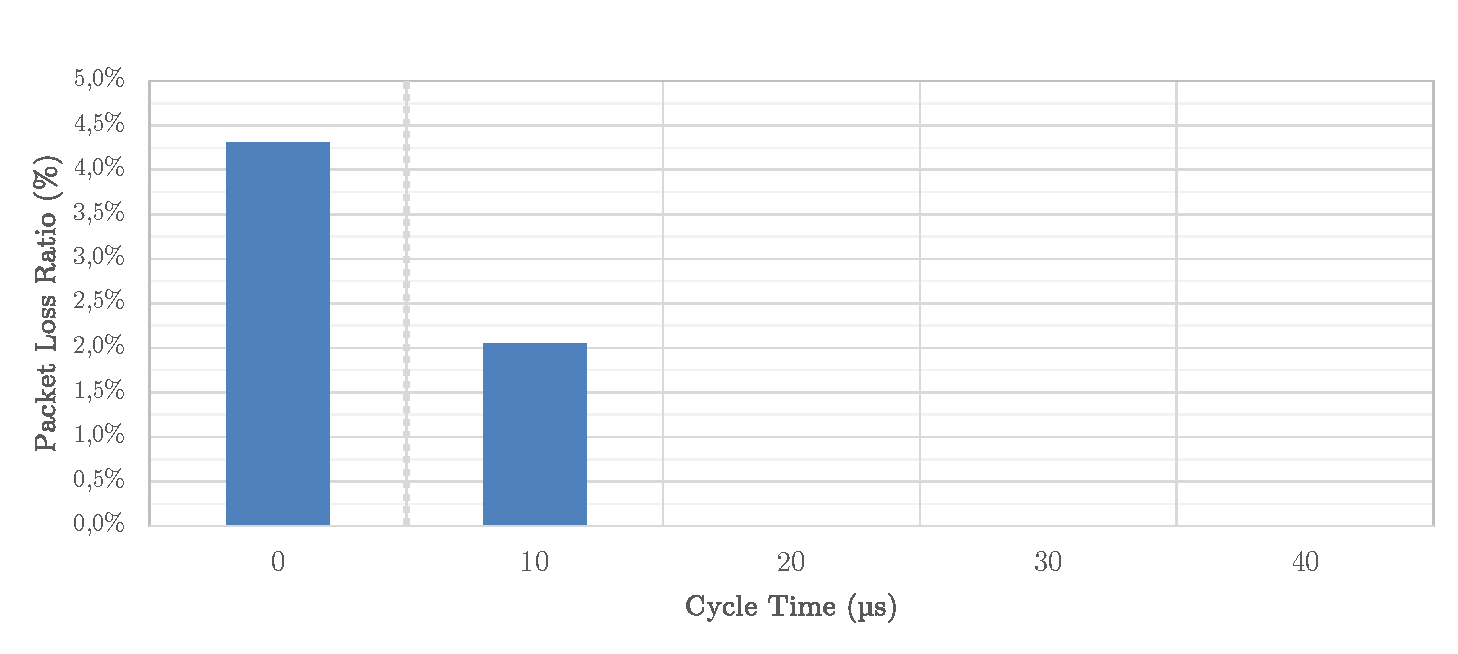
\includegraphics[width=1\textwidth]{figures/reliability/star/rel_d_3a.pdf}
  }
  \subcaptionbox{Datagram Size of 65000 Byte\label{fig:resuc3b}}{%
    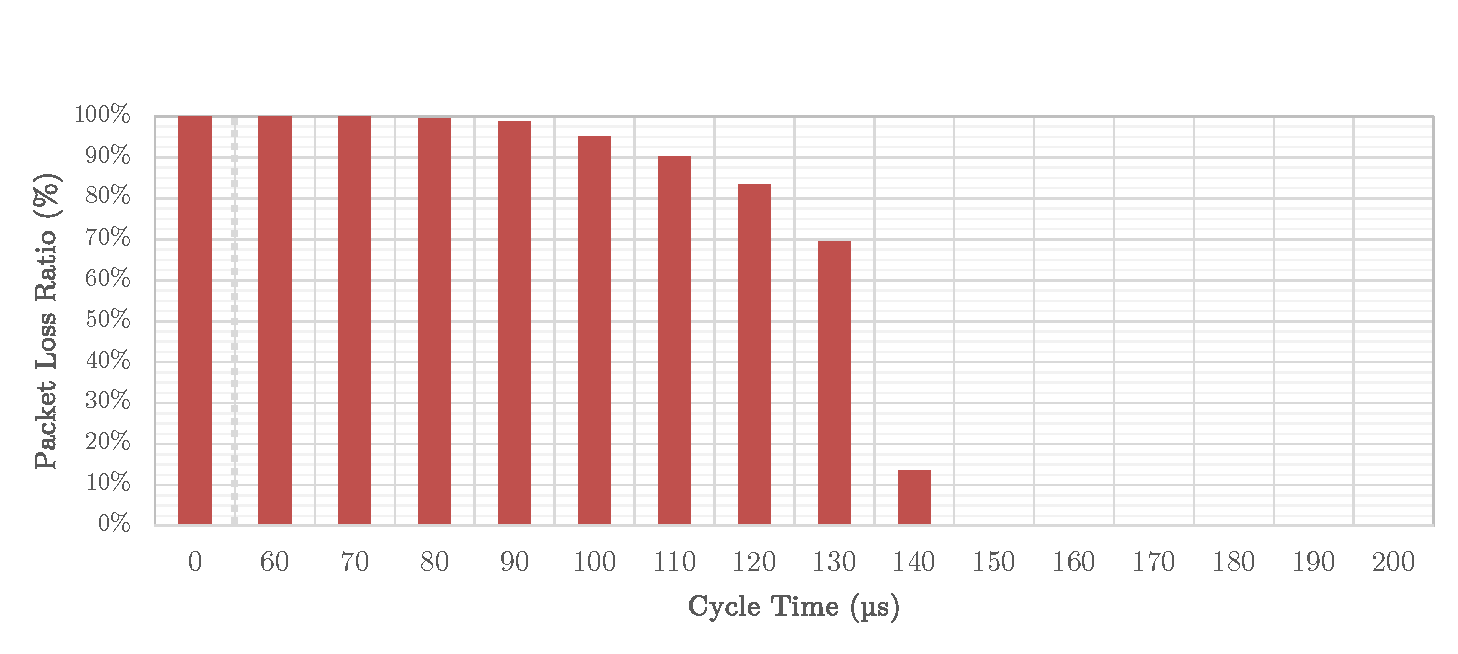
\includegraphics[width=1\textwidth]{figures/reliability/star/rel_d_3b.pdf}
  }
  \caption{Packet Loss Ratio by Cycle Time with High-Performance PCs as System under Test (Campaign `Tests with Realistic Load Scenario').}
  \label{fig:resuc3}
\end{figure}

Figure \ref{fig:resuc3} displays the percentage of packet losses for various cycle times in tests conducted on High-Performance PCs as a system under test. Results are shown for a datagram size of 8900 bytes in \ref{fig:resuc3a} and 65000 bytes in \ref{fig:resuc3b}. No Loses were detected in tests with a datagram size of 80 bytes.

For a datagram size of 8900 bytes, packet losses were detected at cycle times ranging from 0 µs to 30 µs. Notably, significant packet losses of 4.31\% and 2.05\% occurred at 0 µs and 10 µs, respectively, while only isolated losses were observed at 20 µs and 30 µs. For datagrams with a size of 65000 bytes, significantly higher losses were observed. Over 90\% of packet loss occurred up to a cycle time of 110 µs, after which the percentage of packet loss decreases. No losses occurred starting at a cycle time of 210 µs.

The statistics recorded in the examined computer systems (Standard Interface Statistic and Network Stack Statistic) do not indicate any packet drops, so the sender and receiver can be excluded as the source of the loss.

This turns the switch into a possible source of packet loss. The switch has statistics called 'Tail Drops' that can be viewed for each port in the switch's web interface. These reflect the drops that occur when the output queue of a port is full. The switch will discard data until the output queue is cleared again \cite {reli02}. These described drops occurred during the execution of the tests.

For cycle times of 0 µs and 60 µs with a datagram size of 65000 bytes, the losses can be explained by the possible exceeding of the maximum bandwidth of 10 GBit/s. The average throughput in the tests was 9.0 GBit/s and 8.3 GBit/s, which, in combination with the network load in the realistic scenario (2 GBit/s of incoming traffic on HPC2), operates at the maximum bandwidth with which HPC2 is connected to the switch. However, with a 100 µs cycle time, for example, the average throughput is only 5.2 GBit/s, which means that even in combination with the realistic scenario, the maximum bandwidth is not reached. This also applies to packet losses with a datagram size of 8900 bytes.

At 65000 bytes, exceptionally high losses also occur at cycle times of up to 140 µs, even if the available bandwidth is not exceeded, as explained above with 100 µs as an example. Fragmentation may be one reason for this phenomenon of the high losses, since the entire datagram is discarded when a fragment is lost.

In order to better understand the packet losses, certain tests were repeated and the results of the query requests were recorded. This allows the analysis of the temporal occurrence of packet losses.

\begin{figure}[h!]
    \centering
    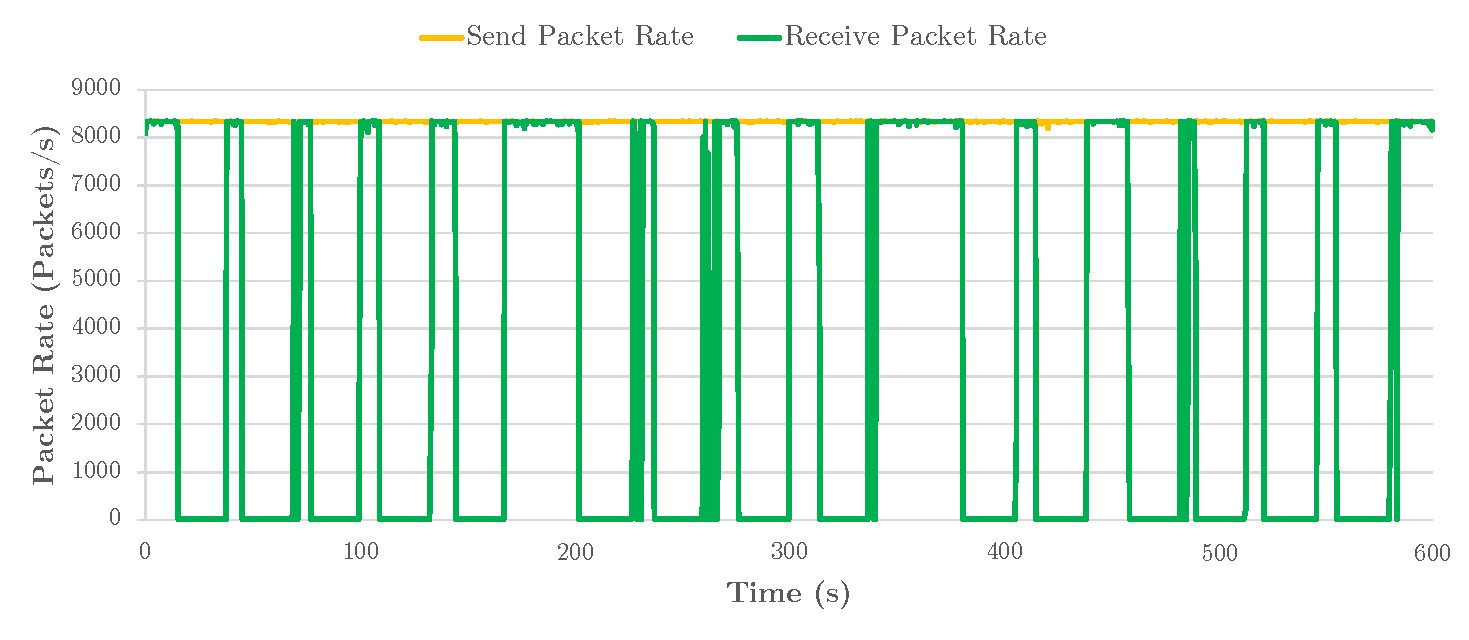
\includegraphics[width=1\linewidth]{figures/reliability/star/rel_d_4.pdf}
    \caption{Sent and Receive Packet Rate over Time for a Test with a Datagram Size of 65000 Byte and a Cycle Time of 120 µs (Campaign `Tests with Realistic Load Scenario').}
    \label{fig:srpr4}
\end{figure}

Figure \ref{fig:srpr4} displays the send and receive packet rate over time for an example test with a datagram size of 65000 bytes and a cycle time of 120 µs. The average throughput was 4.3 Gbit/s, and there was a 61\% packet loss. The variation in packet losses between this implementation and the results presented in \ref{fig:resuc3} for a cycle time of 120 µs can be attributed to fluctuations.

The diagram shows that the packet losses occur cyclically. It is illustrated that there are phases during which all packets are lost and phases during which nearly all packets are received. These phases of packet loss have a constant duration of 25 seconds, but the interval between these phases varies.

Based on recorded data, it can be concluded that the packet losses occurred due to an overload the switch. The recorded pattern with the constant loss intervals could indicate an kind of overload protection mechanism of the switch, which prevents the sending of packets. However, the Ethernet switch is a 'Black Box', as Cisco does not publish detailed information about the implementation, so the exact cause of the losses cannot be analyzed further. During the tests, all protection mechanisms of this kind, which can be set in the switch interface, were deactivated.

\paragraph{Classification of Results}
This campaign showed that packet losses can occur when the setup is loaded with the realistic scenario. Losses were also observed below the maximum bandwidth. The reason for this is most likely due to switch congestion, which occurs cyclically.

\subsubsection{Tests with Realistic Load Scenario and Quality of Service}
\paragraph{Motivation and Context}
This test campaign examines the impact of using Quality of Service on the result. The IP header's Differentiated Services field is utilized for this purpose. The TestSuite specifies a priority of 63 for its communication, which is the highest possible value. The switch is also configured to prioritize packets with this priority.

The realistic scenario is executed on all systems involved in the setup, as in the previous campaign. The network traffic generated as part of the scenario is not given preferential treatment by the switch, as no priority is assigned to it.

The test procedure selected for this campaign is the same as the one used for the 'Tests with Realistic Load Scenario' campaign (see \ref{chap:campaignloadscen}). Datagram sizes of 80 bytes, 8900 bytes, and 65000 bytes were taken into consideration. The system under test includes both the High-Performance PCs and the Traffic PCs.

The test campaign examined not only the Intel X710-T2L network interfaces that are the default for the topology, but also the Intel X540-T2, the Inspur X540-T2 and the Lenovo QL41134, which were tested with the High-Performance PCs as the system under test.

\paragraph{Results}
In tests with the High-Performance PCs, no packet loss was detected for all datagram sizes tested, with the smallest cycle time tested of 0 µs for 80, 8900, and 65000 bytes. The average throughput achieved in these tests was 91.5 MBit/s for 80 bytes, 7.23 GBit/s for 8900 bytes, and 9.01 GBit/s for 65000 bytes. There were no packet losses in the tests with the alternative network cards (Intel X540-T2, Inspur X540-T2 and Lenovo QL41134). The achieved average throughput in these tests is similar to that of the Intel X710-T2L.

Also, no packet loss was detected in the tests with the Traffic PCs with the shortest cycle time. The average throughputs were 52.1 MBit/s for 80 bytes, 4.88 GBit/s for 8900 bytes, and 7.41 GBit/s for 65000 bytes. This also shows that, as mentioned in the first campaign (see \label{chap:relcamp1}), the system load of the traffic PCs has a greater influence on the average throughput achieved by the sender.

However, packet losses were detected in all tests for the traffic generated by iPerf in the context of the realistic load scenario. These effects were caused by the switch, as shown by its statistics.

\paragraph{Classification of Results}
The campaign has demonstrated that reliability can be ensured through the use of quality of service. However, this requires traffic to be prioritized. Nevertheless, packet losses were detected in non-prioritized traffic. Currently, the Distributed Test Support System does not provide such prioritization, so no QoS can be applied.

Another finding from this campaign is that the two computer systems in the system under test (client and server) do not cause any packet losses even when under stress from the realistic scenario. This confirms the assumption made in the previous campaign 'Tests with Realistic Load Scenario' based on the recorded statistics.

Furthermore, the campaign has shown that the Intel X540-T2, Inspur X540-T2 and Lenovo QL41134 network interfaces have comparable reliability to the Intel X710-T2L.

\subsubsection{Tests with Realistic Load Scenario and Custom Network Load Generator}
\paragraph{Motivation and Context}
The `Tests with Realistic Load Scenario' campaign (see \ref{chap:campaignloadscen}) has already concluded that the switch suffered from an overload situation. The purpose of this campaign is to further analyze the circumstances that led to packet loss in the switch.

One possible reason for the occurrence of packet losses through the switch is the bursts sent by the network traffic generated by iPerf for the realistic scenario, which cause a short-term overload of the switch. This assumption is supported by the observation that packet losses occur in the switch when executing the realistic scenario in the test setup, even without running a test campaign. Due to the specified bandwidth of 1 GBit/s per channel in the realistic scenario, it is expected that no packet losses will occur as the network's maximum bandwidth is significantly higher.

iPerf utilizes a throttling algorithm to regulate the specified bandwidth. This algorithm monitors the data throughput sent at 100 ms intervals and adjusts it as needed to maintain specified bandwidth \cite{reli03}. Unlike CPU stressors, which run as real-time processes in a realistic load scenario, iPerf is not executed as a real-time process on the system. This can result in iPerf not being allocated sufficient computing time. As a result, the throttling algorithm may make extreme adjustments to achieve the required bandwidth, which may result in data bursts being sent. However, it is not possible to verify this assumption by recording with Wireshark due to hardware limitations.

In this test campaign, a self-programmed network traffic generator based on TestSuite replaces iPerf in the realistic load scenario. Unlike iPerf, this generator does not use a throttling algorithm and therefore does not send any bursts. Furthermore, the process is executed in real-time with a priority of 90, which is higher than that of the stressors but lower than that of TestSuite. The cycle time was configured to ensure a maximum transmission bandwidth of 1 GBit/s.

The test procedure for this campaign was the same as for the 'Tests with Realistic Load Scenario' campaign (see \ref{chap:campaignloadscen}). Datagram sizes of 80 bytes, 8900 bytes, and 65000 bytes were considered. Tests were performed exclusively with the High-Performance PCs as the system under test. Quality of Service was not utilized.

\paragraph{Results}

\begin{figure}[h!]
    \centering
    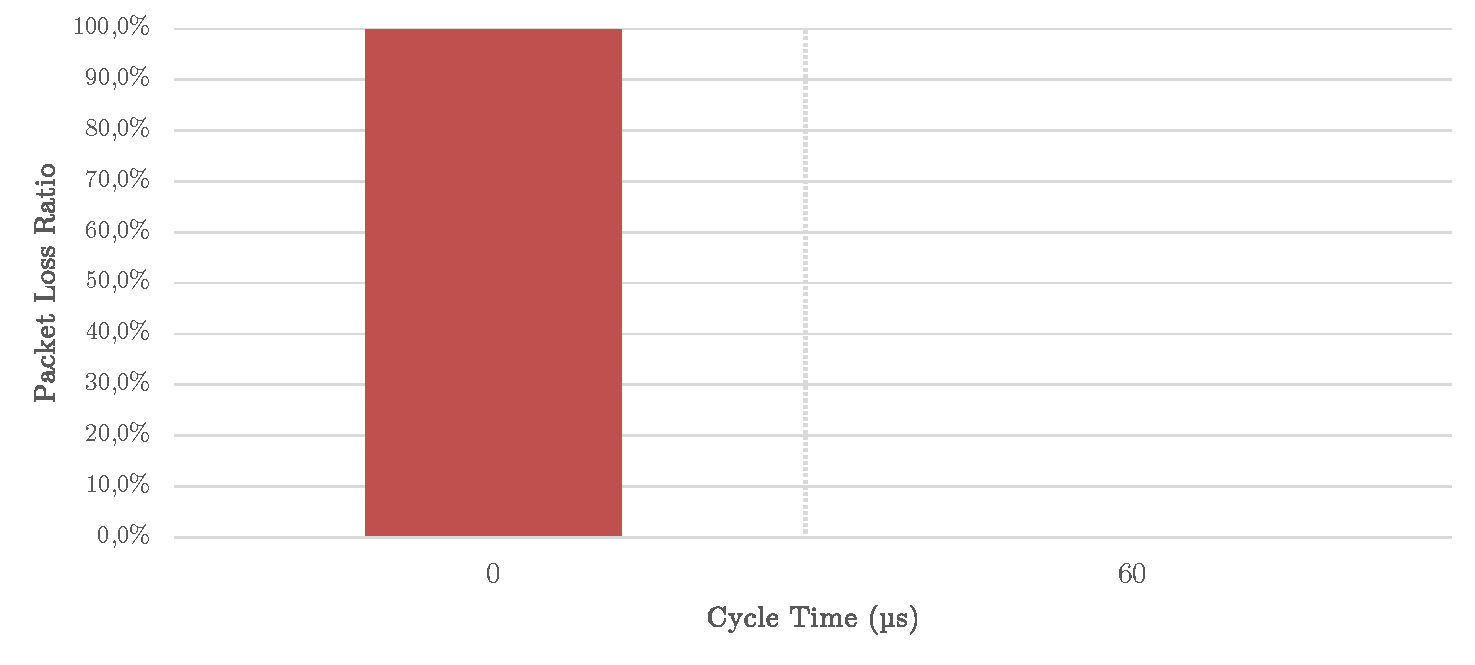
\includegraphics[width=1\linewidth]{figures/reliability/star/rel_d_5.pdf}
    \caption{Packet Loss Ratio by Cycle Time for a Datagram Size of 65000 Byte with High-Performance PCs as System under Test (Campaign `Tests with Realistic Load Scenario and Custom Network Load Generator').}    \label{fig:srpr5}
\end{figure}

During the campaign, only packet losses were observed when examining a datagram size of 65000 bytes. At a cycle time of 0 µs, packet losses of 99.9\% were recorded. while no packet losses occurred at a cycle time of 60 µs. These results are illustrated in Figure \ref{fig:srpr5}. It is worth noting that packet drops were again only reported by the switch.

A major reason for the high number of packet losses at 65000 byte datagram size and 0 µs cycle time is the fact that the maximum bandwidth of 10 Gbps is exceeded, as the average throughput in the test is 9.1 Gbps. Additionally, packet loss is increased by the use of fragmentation.

\paragraph{Classification of Results}
Compared to using iPerf (see \ref{chap:campaignloadscen}), a separate network stressor significantly reduces packet losses. This suggests that iPerf generates bursts that overload the switch and cause packet loss. However, it should be noted that the systems in the Distributed test support system are asynchronous, meaning they can also send out bursts that should not overload the network.

\subsection{Insights}
The investigation of the star topology with a switch in the center has revealed that an Ethernet switch is unsuitable for use in the Distributed Test Support System. The switch was found to be the cause of packet loss, particularly in connection with burst traffic.

Another concern is that the maximum bandwidth at which each participant is connected to the switch may be exceeded. Since the Distributed Test Support System is an arrangement of independent systems, such an exceedance cannot be excluded.

Regarding the computer systems, the investigation showed that a memory load that provokes a constant memory overflow can lead to packet loss. However, it was also found that both High-Performance PC and Traffic PC systems do not experience packet losses when subjected to a load similar to that in a real Test Support System.

Furthermore, in addition to the standard network interfaces in the topology, the Intel X540-T2, Inspur X540-T2, and Lenovo QL41134 network interfaces were also examined, and no reduction in reliability based on packet loss was found, making them equally suitable for use in a Distributed Test Support System.



\clearpage
\section{Reliability Analysis of the Star Topology with the iHawk in the Center} \label{chap:ReliabIhawk}

\subsection{System under Test} \label{chap:ReliabIhawk:SuT}
The key takeaway from the previous reliability tests (see \ref{chap:switchtest}) is that the use of an Ethernet switch in the Distributed Test Support System is unsuitable, as it leads to a significant number of lost packets. Additionally, the behavior of the switch was found to be unreliable and unpredictable. As a result, an alternative topology was developed and investigated, which is described in \ref{chap:TopoiHawk}, and in which the iHawk is placed in the center of the star.

In this configuration, all participants (hereafter referred to as Endpoints) are connected to a computer system in the center (hereafter referred to as the Center). In a practical implementation in the test system, the endpoints are the I/O PCs and the center is an iHawk. The endpoints are not connected to each other, as communication in the Distributed Test Support System is mainly between the center and the endpoints, rather than between the endpoints themselves.

For the test setup, the High-Performance PCs and Traffic PCs serve as endpoints, while an iHawk is located in the center. Unless otherwise specified, the network cards mentioned in the presenation of the topology (see \ref{chap:TopoiHawk}) will be used for the tests.

The system under test for subsequent test campaigns is no longer a single communication that is examined. Instead, the TestSuite examines each bidirectional link in the topology. Since each of the four endpoints is connected to the center by two bidirectional links, there are 16 UDP communications generated and measured by the TestSuite.

\begin{figure}[h!]
    \centering
    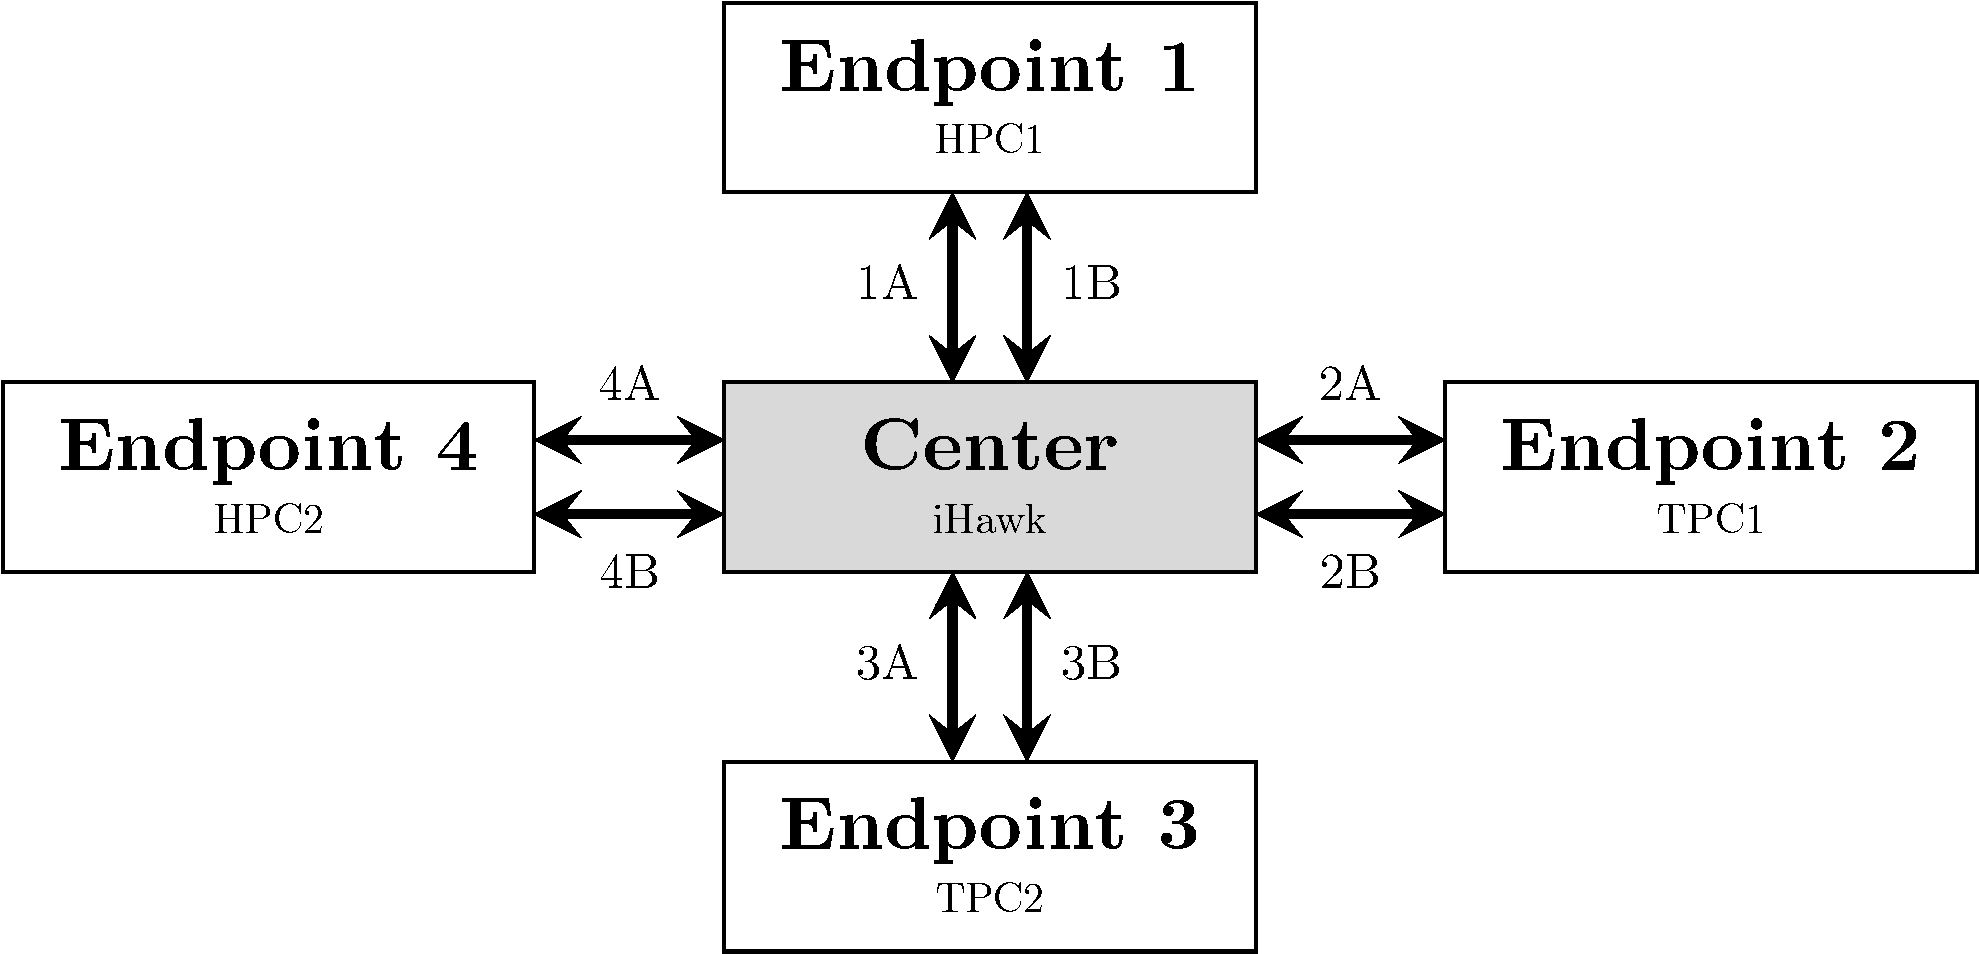
\includegraphics[width=0.8\linewidth]{figures/reliability/ihawk/topo.pdf}
    \caption{Structure and Nomenclature of Communication Channels of the Test Setup with the iHawk in the Center of the Star.}
    \label{fig:topoihawknaming}
\end{figure}

To distinguish between communications more easily, the nomenclature scheme depicted in Figure \ref{fig:topoihawknaming} was designed. The two physical 10 GbE links that connect each endpoint to the centers are referred to as link `\textbf{A}' and `\textbf{B}'. A separate TestSuite process generates and measures UDP communication in both directions across each of these links simultaneously. These directions are referred to as `\textbf{H}' and `\textbf{R}'. Direction `H' refers to communication channels where the center is the sender and the endpoint is the receiver. Conversely, direction `R' refers to communication channels where the center is the receiver and the endpoint is the sender.

Because 16 bidirectional communications lead to a high network load, especially in the center, the settings recommended by Intel for high performance and reliability in the Linux Performance Tuning Guide for the Ethernet 700 Series \cite{intermod03} were used. These settings were chosen based on experiments conducted with the High-Performance PCs prior to this campaign. These settings include:
\begin{itemize}
  \item Disabling of Energy Efficient Ethernet
  \item Enlargement of the RX\_Ring and TX\_Ring to 4096 slots
  \item Deactivation of Interrupt Moderation (unless otherwise specified)
  \item UDP Receive Buffer Size of 25 MB
\end{itemize}

\subsection{Test Campaigns}

\subsubsection{Tests without additional Load} \label{chap:noaddloadTest}
\paragraph{Motivation and Context}
This test campaign aims to assess the reliability of the setup when all 16 communication channels are operating at full capacity. The center, which has to handle a high communication load, is the main focus of the campaign.

To analyze the reliability in a long-term test, a test duration of 2 hours is used. Datagram sizes of 80 bytes, 8900 bytes and 65000 bytes are tested and a cycle time of 0 µs is selected, which corresponds to an uninterrupted transmission process.

\paragraph{Results}
\subparagraph{System Utilization}
Before presenting the results on reliability based on the number of packet losses, this section discusses the utilization of the systems, especially the utilization of the iHawk in the center.

\begin{figure}[h!]
    \centering
    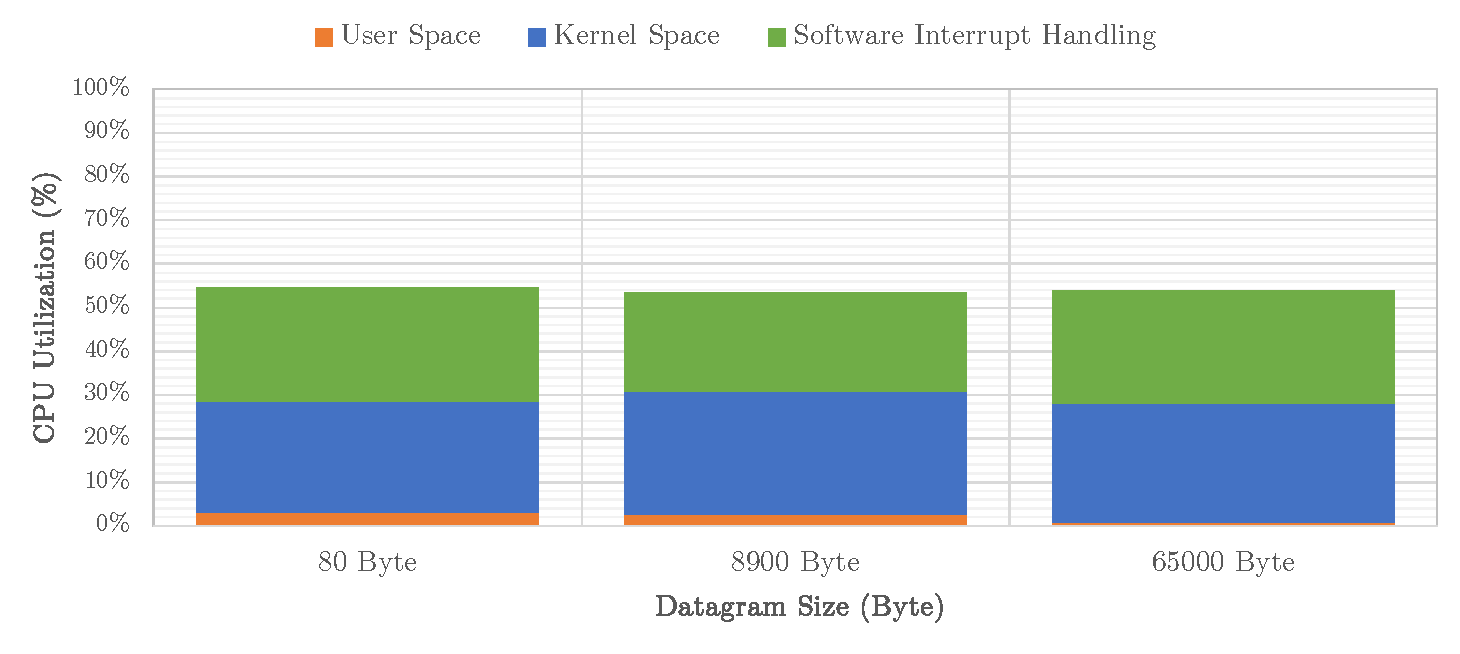
\includegraphics[width=1\linewidth]{figures/reliability/ihawk/diagr2.pdf}
    \caption{CPU Utilization in the Center for the examined Datagram Sizes (Campaign `Tests without additional Load').}
    \label{fig:diagr2CPU}
\end{figure}

Figure \ref{fig:diagr2CPU} displays the average CPU utilization at the center for the examined datagram sizes. The overall utilization across all datagram sizes is about 55\% and varies slightly. As the datagram size increased, the utilization in the user space decreased while the utilization in the kernel space increased. Additionally, utilization was also observed in the software interrupt handling area.

The increased user space utilization, especially for datagrams with a size of 80 bytes, is due to the higher number of packets generated or retrieved in the application (TestSuite). While about 100,000 packets per second are processed with an 80 byte datagram size, only about 19,000 packets per second are processed with a 65,000 byte datagram size.

The utilization in the software interrupt handling area includes packet processing during reception and partially during transmission. The lowest utilization is measured with a datagram size of 8900 bytes, because fewer packets are processed (compared to 80 bytes) and no fragmentation or defragmentation is performed (compared to 65000 bytes).

The CPU utilization was monitored throughout the testing period and no anomalies were detected. A fluctuation of ±3\% of the reported average utilizations can be observed. The CPU load does not indicate any overloading of the iHawk in the center during the test.

CPU utilization at the endpoints was also considered. The High-Performance PCs showed an overall utilization of 14.8\%, while the Traffic PCs showed a higher utilization of 34.3\% due to their inferior hardware specifications. Again, there was little variation in the overall utilization between the datagram sizes tested. Based on the CPU utilization, no overload can be detected on the endpoints either.

\subparagraph{Packet Loss}

\begin{figure}[h!]
    \centering
    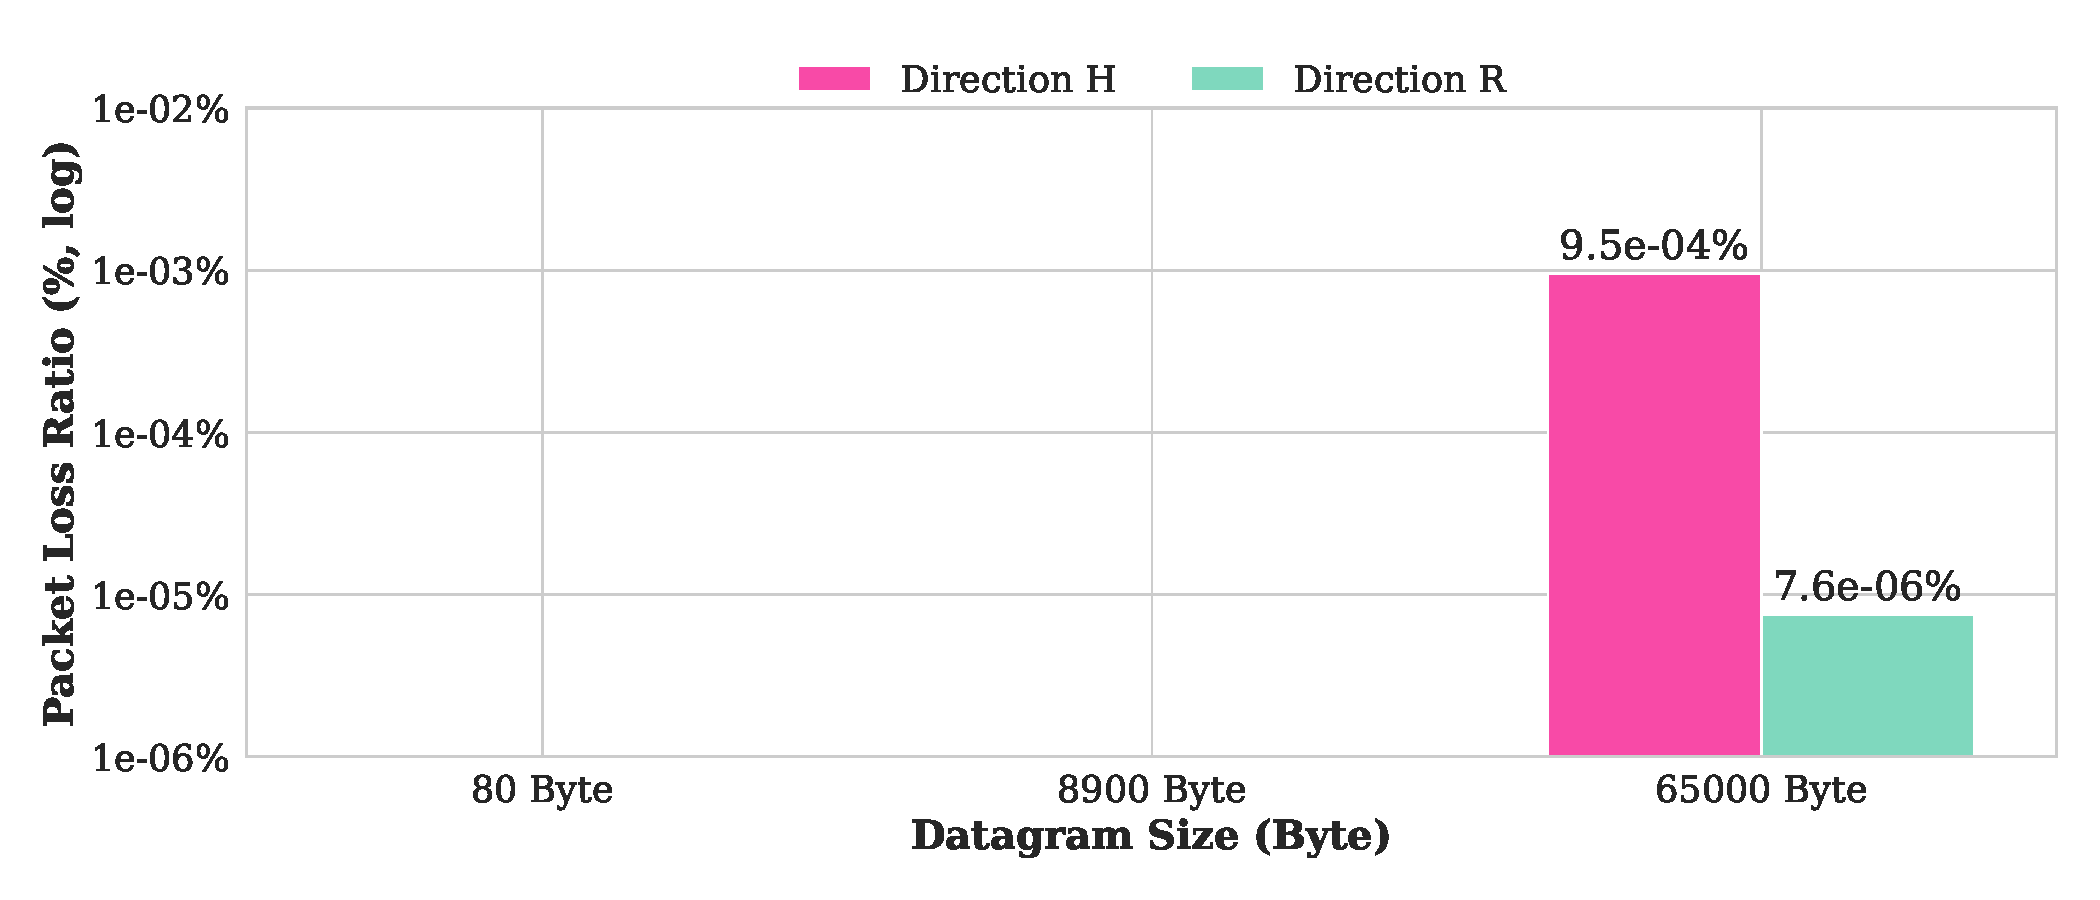
\includegraphics[width=1\linewidth]{figures/reliability/ihawk/diagr3.pdf}
    \caption{Packet Loss Ratio by Datagram Size and Communication Direction (Campaign `Tests without additional Load').}
    \label{fig:diagr3Loss}
\end{figure}

Figure \ref{fig:diagr3Loss} displays the overall packet loss ratio for this test campaign, categorized by datagram size and communication direction. No packet losses were observed during the tests conducted with datagram sizes of 80 and 8900 bytes. However, packet losses were observed in both the `H' and `R' directions during testing with a datagram size of 65000 bytes when using fragmented packets. Table \ref{tab:LossesC1} presents a breakdown of the losses by channel. The packet losses in the `H' and `R' directions will be analyzed separately separately below.

\begin{table}[h!]
\centering
\newcolumntype{C}[1]{>{\raggedright\arraybackslash}p{#1}}

\begin{subtable}{\linewidth}
\centering
\begin{tabular}{l| C{2.3cm} C{1.2cm} | l}
	\toprule
	\textbf{Channel} & \multicolumn{2}{l|}{\textbf{Lost Packets}} & \textbf{Average Throughput} \\
	\scriptsize{ }& \multicolumn{2}{l|}{\scriptsize{(Ratio/Total)}} & \scriptsize{ }\\
	\midrule
 	1A-H & \num{0} \% & / 0    & 9.90 GBit/s \\ 
 	1B-H & \num{0} \% & / 0    & 9.90 GBit/s \\
 	2A-H & \num{0} \% & / 0    & 9.89 GBit/s \\
 	2B-H & \num{0} \% & / 0    & 9.89 GBit/s \\
 	3A-H & \num{3.9e-03} \% & / 4313 & 9.89 GBit/s \\
 	3B-H & \num{3.8e-03} \% & / 4285 & 9.89 GBit/s \\
 	4A-H & \num{0} \% & / 0    & 9.90 GBit/s \\
 	4B-H & \num{0} \% & / 0    & 9.90 GBit/s \\
	\bottomrule
\end{tabular}
\caption{Direction `H'}
\label{tab:LossesC1:H}
\end{subtable}
\vspace{6pt}

\begin{subtable}{\linewidth}
\centering
\begin{tabular}{l|C{2.3cm} C{1.2cm}|l}
	\toprule
	\textbf{Channel} & \multicolumn{2}{l|}{\textbf{Lost Packets}} & \textbf{Average Throughput} \\
	\scriptsize{ }& \multicolumn{2}{l|}{\scriptsize{(Ratio/Total)}} & \scriptsize{ }\\
	\midrule
	1A-R & \num{5.0e-06} \% & / 7  & 8.25 GBit/s \\ 
 	1B-R & \num{9.1e-06} \% & / 11 & 8.75 GBit/s \\
	2A-R & \num{5.8e-06} \% & / 8  & 8.23 GBit/s \\
 	2B-R & \num{5.8e-06} \% & / 8  & 8.13 GBit/s \\
 	3A-R & \num{5.1e-06} \% & / 7  & 8.12 GBit/s \\
 	3B-R & \num{1.1e-05} \% & / 16 & 8.09 GBit/s \\
 	4A-R & \num{7.9e-06} \% & / 9  & 8.20 GBit/s \\
 	4B-R & \num{7.8e-06} \% & / 9  & 8.40 GBit/s \\
	\bottomrule
\end{tabular}
\caption{Direction `R'}
\label{tab:LossesC1:R}
\end{subtable}

\caption{Packet Losses and Average Throughput for a Datagram Size of 65000 Bytes (Campaign `Tests without additional Load').}
\label{tab:LossesC1}
\end{table}


Packet losses of \num{7.56e-6} \% were observed when examining a datagram size of 65000 bytes in the direction from the endpoints to the center (`R'). Table \ref{tab:LossesC1:R} provides a breakdown of these losses at a datagram size of 65000 bytes by channel, which shows that few losses occur in all communication channels in this direction and are almost evenly distributed among the individual channels.


\begin{figure}[h!]
    \centering
    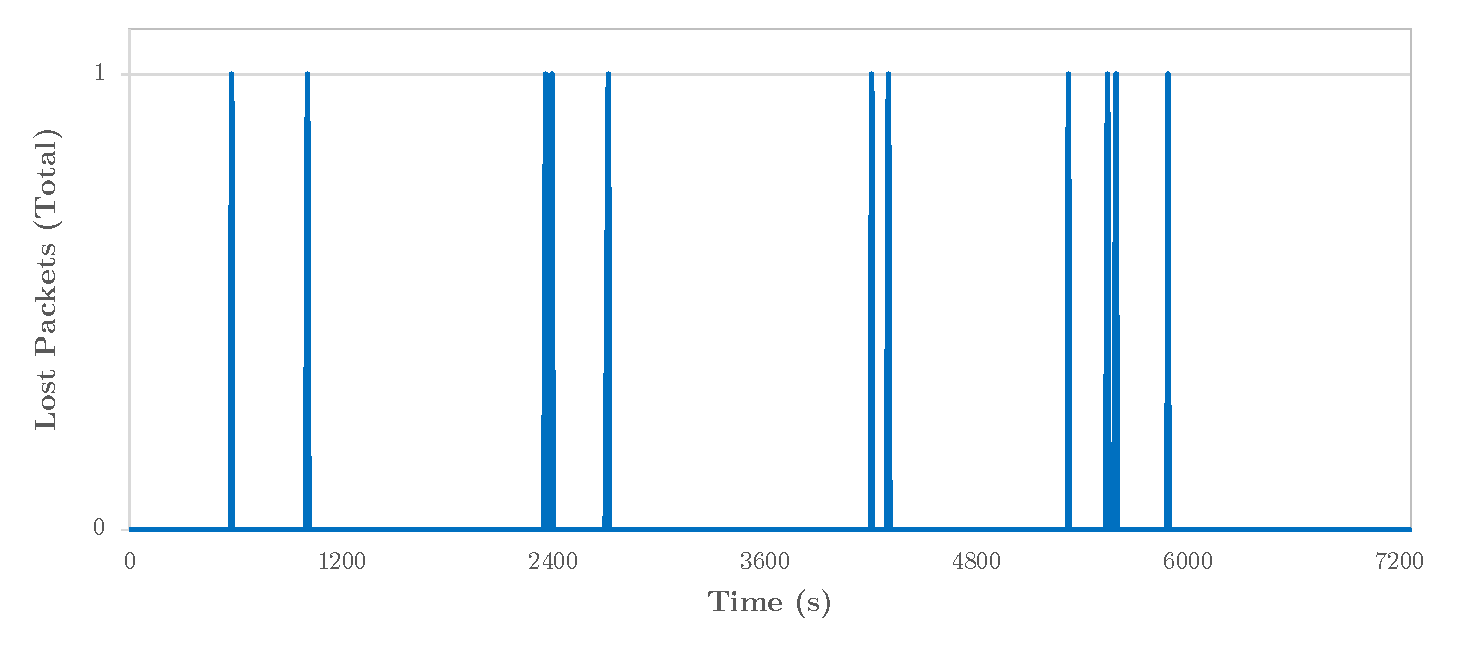
\includegraphics[width=1\linewidth]{figures/reliability/ihawk/diagr4.pdf}
    \caption{Temporal Distribution of Packet Loss for Channel 1B-R (Campaign `Tests without additional Load').}
    \label{fig:diagr4Temp}
\end{figure}

Figure \ref{fig:diagr4Temp} displays the temporal distribution of packet losses using channel 1B-R as an example. It is evident that the packet losses do not occur in bursts, but instead are distributed independently across the entire test duration. This trend can observed for the other channels.

Packet losses can occur at the sender (Endpoints in the `R' direction), during cable transmission on the route, or at the receiver (Center in the `R' direction). Further investigation is necessary to determine the precise location and reasons for packet losses, as the statistics of the network interfaces and the network stack on all computer systems for this direction do not indicate any drops.

To investigate the losses in the direction `R' at 65,000 bytes, test sessions of 20 minutes were run, gradually reducing the number of bidirectional links used until no losses occurred. The results of this investigation are displayed in Figure \ref{fig:diagr5Loss}.

\begin{figure}[h!]
    \centering
    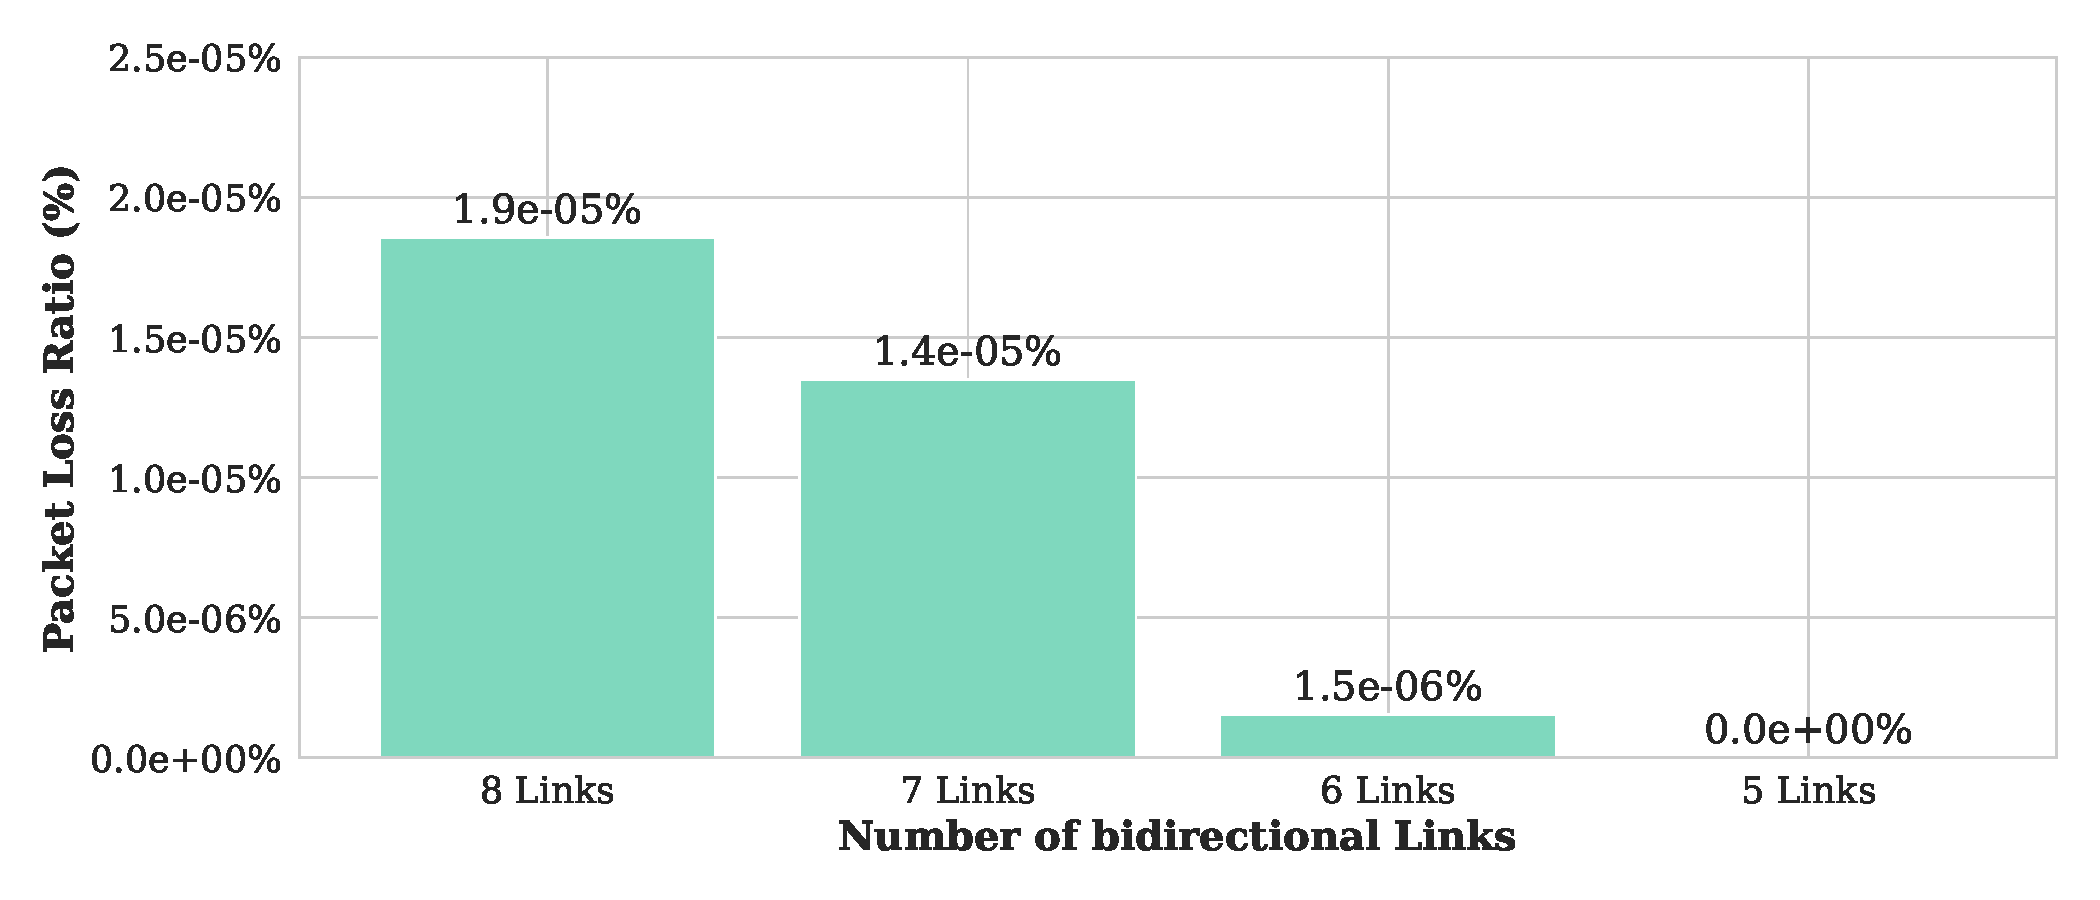
\includegraphics[width=1\linewidth]{figures/reliability/ihawk/diagr5.pdf}
    \caption{Packet Loss Ratio by Number of Links with a Datagram Size of 65000 Byte in Direction `R' (Campaign `Tests without additional Load').}
    \label{fig:diagr5Loss}
\end{figure}

The investigation shows that there are no losses in the direction `R' when using 5 bidirectional links. The ratio of losses to the total number of packets decreases as the number of links decreases.

In this test campaign, only the number of links decreased, but the configuration of the TestSuite remains unchanged. Therefore, the load on a single link remains the same, so the route cannot be considered the cause of the packet losses. In the test with five bidirectional links, endpoints 1 and 4 utilize both of their respective links, while endpoint 2 only utilizes link A. Endpoint 3 is not part of this test. Since the load on endpoints 1 and 4 is the same as in the original scenario with eight links, the senders, in this case the endpoints, are not considered to be responsible for the packet losses.

Based on these findings, it can be concluded that the receiver, in direction `R' the center, is where the packet losses occurred. Observing that losses occur only at a datagram size of 65000 bytes suggests a correlation with the defragmentation on the network stack. One possible scenario is an overflow of the buffer allocated for defragmentation, resulting in packet losses. \\


As displayed in figure \ref{fig:diagr3Loss}, the direction `H' from the center to endpoints experiences significantly higher packet loss at a rartio of \num{9.55e-4} \% for a datagram size of 65000 bytes compared to direction `R'. Table \ref{tab:LossesC1:H} includes a breakdown of the packet losses for a datagram size of 65000 bytes by channel. It is important to note that only packet losses were observed in communications with endpoint 3.

The statistics (Standard Interface Statistic and Network Stack Statistic) recorded in the sender (Center) show no losses. In contrast, the statistics for the affected receiver (Endpoint 3) show packet losses in the \texttt{rx\_missed\_errors} counter of the Standard Interface Statistic (see Table \ref{tab:ep3InterfaceStat}).

\begin{table}[h]
\centering
\begin{tabular}{l|l|l|l}
	\toprule
	\textbf{Interface} & \textbf{Channel} & \textbf{\texttt{rx\_dropped}} & \textbf{\texttt{rx\_missed\_errors}} \\
	\midrule
 	enp1s0f0 & 3A-(H/R) & 0 & 19507 \\ 
 	enp1s0f1 & 3B-(H/R) & 0 & 19414 \\
	\bottomrule
\end{tabular}
\caption{Extract of the Standard Interface Statistic for Endpoint 3.}
\label{tab:ep3InterfaceStat}
\end{table}

According to the Linux kernel documentation, \texttt{rx\_missed\_errors} indicates the number of packets that were dropped by the computer due to insufficient space in the buffer \cite{sock11}. This indicates that the computer may not be able to handle incoming packets at the rate at which they arrive at the network interface, resulting in network congestion at the endpoint 3. The ksoftriq threads, which handle the processing of incoming packets as described in \label{chap:recpath} were unable to process all the packets available in the network device's ring buffer before their CPU time expired.

The recorded losses of the TestSuite are lower than the values for \texttt{rx\_missed\_error}. This is due to the fact that losses only occurred at 65000 bytes, where the UDP packets were fragmented into 8 IP packets due to the configured MTU of 9000 bytes. If a fragment is lost, the entire packet is discarded.

\begin{figure}[h!]
    \centering
    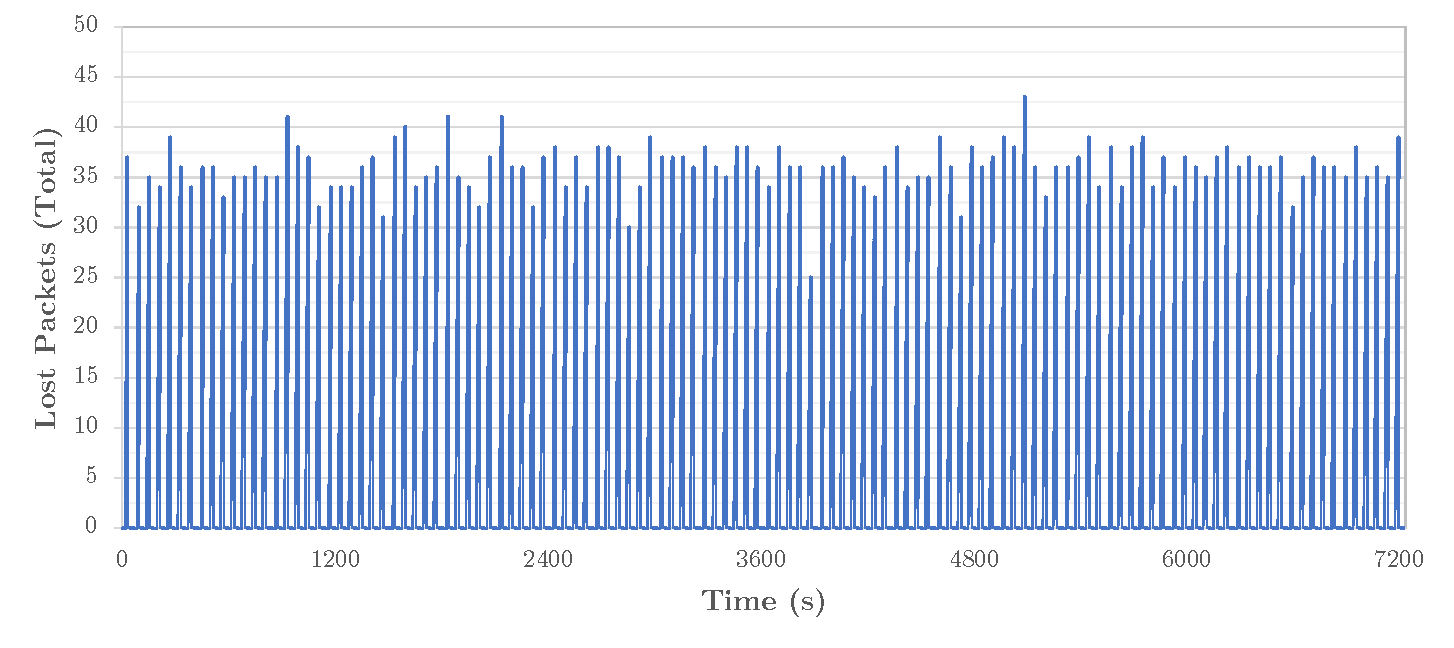
\includegraphics[width=1\linewidth]{figures/reliability/ihawk/diagr6.pdf}
    \caption{Temporal Distribution of Packet Loss for Channel 3A-H (Campaign `Tests without additional Load').}
    \label{fig:diagr6Temp}
\end{figure}

Figure 3 shows the temporal distribution of packet losses for communication 3A-H. The graph uses a resolution of 100,000 packets.  It is clear that packet losses occur uniformly over time rather than in bursts. Furthermore, it can be observed that losses are cyclic in nature. Upon examining the individual query requests, it is noticeable that there is a packet loss of approximately 30 to 40 packets every 900,000 packets (~65 seconds), but no packets are lost in the intervening period. The graph for 3B-H shows comparable results.

These results confirm the hypothesis of network congestion on endpoint 3, which where already assumed in the presentation of the standard interface statistics (see Table \ref{tab:ep3InterfaceStat}). However, there is no indication of CPU overload, as the average CPU utilization on endpoint 3 during this test was 36.7\%. An additional investigation focusing on endpoint 3 revealed no packet loss when using only one bidirectional link with this endpoint.

It is also important to note that packet losses are only observed on endpoint 3. Endpoint 2 and endpoint 3 belong to the Traffic PC system type (refer to \ref{chap:ComputerHardware}), meaning they utilize the same CPU and are equipped with the Intel X540-T2 network card. The recorded average CPU utilization of both computers during the test  was also almost identical.

The primary distinction between the two Traffic PCs is the motherboard. TPC1 (Endpoint 2) uses a GA-Z77X-UD5H motherboard, while TPC2 (Endpoint 3) is equipped with a GA-Z77X-UD3H motherboard. Although both motherboards have the PCIe x16 slot, which is used for the network card, connected directly to the CPU and feature the same Intel X77 chipset, there are still differences in the components and their cooling, which is more advanced on the GA-Z77X-UD5H \cite{reli04, reli05}.

Both computer systems are equipped with air cooling to provide heat dissipation to the CPU. However, TPC1 is equipped with a superior type of air cooling. As a result, the CPU of TPC2 may be subjected to higher temperatures compared to TPC1, which could lead to CPU throttling. This could be a possible explanation for the differences in packet loss observed between endpoints 2 and 3.

Table \ref{tab:LossesC1:H} shows that there were no losses observed in the `H' direction with the High-Performance PCs.

\paragraph{Classification of Results}

The results indicate that packet losses occur in the test setup when using all bidirectional links, both in the center and in endpoint 3 due to congestion. However, it should be noted that these losses are relatively modest and occur only at maximum load and only in conjunction with a datagram size of 65000 bytes with fragmentation.

\subsubsection{Tests with additional Load at the Center}

\paragraph{Motivation and Context}
The purpose of this test campaign is to analyze the reliability of the system under additional load at the center. The realistic scenario described in \ref{chap:campaignloadscen} was used as the additional system load. The number and intensity of stress-ng stressors on the computer system remain the same. However, no network stressors were used because the network load is entirely generated and measured by the TestSuite.

A test duration of 10 minutes was chosen. To maintain consistency with the prior campaign, datagrams sizes of 80, 8900, and 65000 bytes were tested. Despite packet loss in the previous scenario, a cycle time of 0 µs was again selected to evaluate the system under a high network load. All 16 communication channels were utilized.

\paragraph{Results}

\begin{figure}[h]
    \centering
    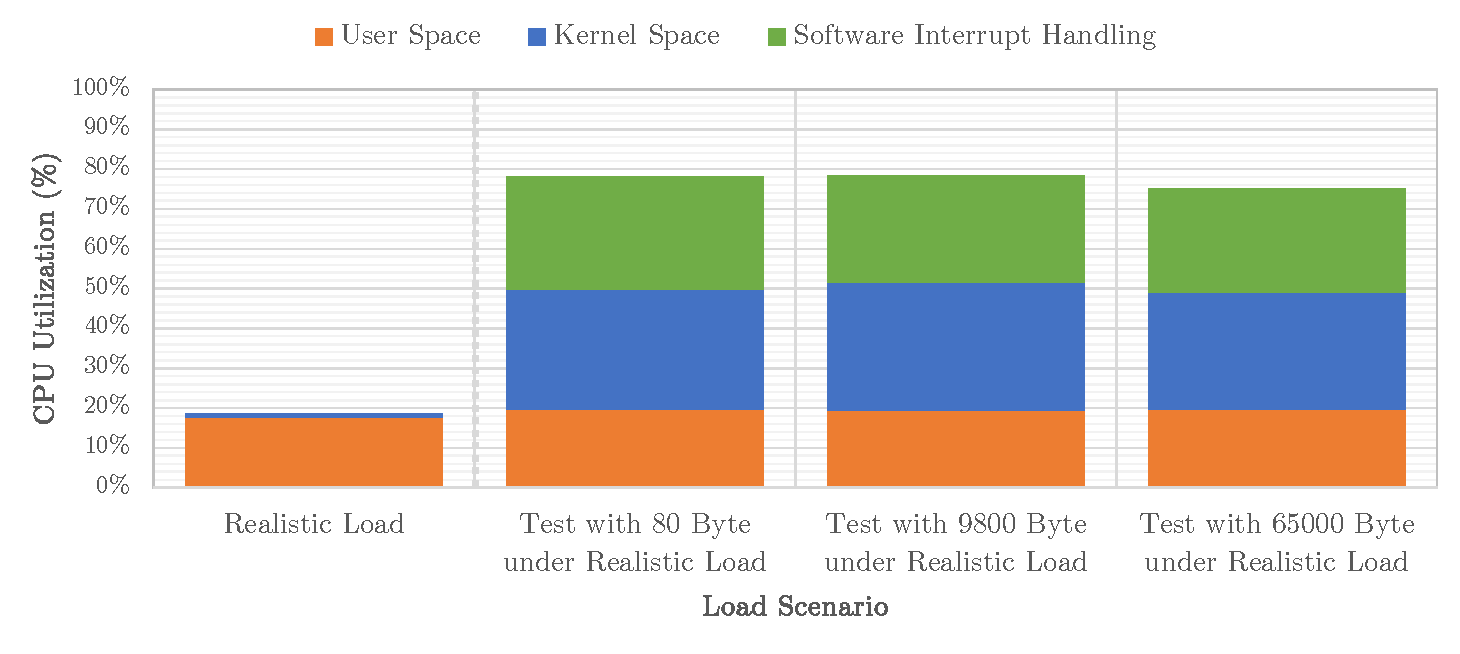
\includegraphics[width=1\linewidth]{figures/reliability/ihawk/diagr7.pdf}
    \caption{CPU Utilization in the Center for different Load Scenarios (Campaign `Tests with additional Load at the Center').}
    \label{fig:diagr7CPU}
\end{figure}

Figure \ref{fig:diagr7CPU} displays the average CPU utilization in the center during the execution of this test campaign and compares it with the execution of the realistic load scenario without running the tests with the TestSuite.

The realistic scenario utilizes 18.6\% of the CPU. The majority of the CPU time is spent in the user space with 17.6\% and 1\% is spent in the kernel space. The average CPU utilization during the execution of the test campaign is between 72\% and 78\%. No overload situation due to the additional system load can be identified when examining CPU utilization. Additionally, the transmission data transfer rate is also not affected by the additional load.

\begin{figure}[h]
    \centering
    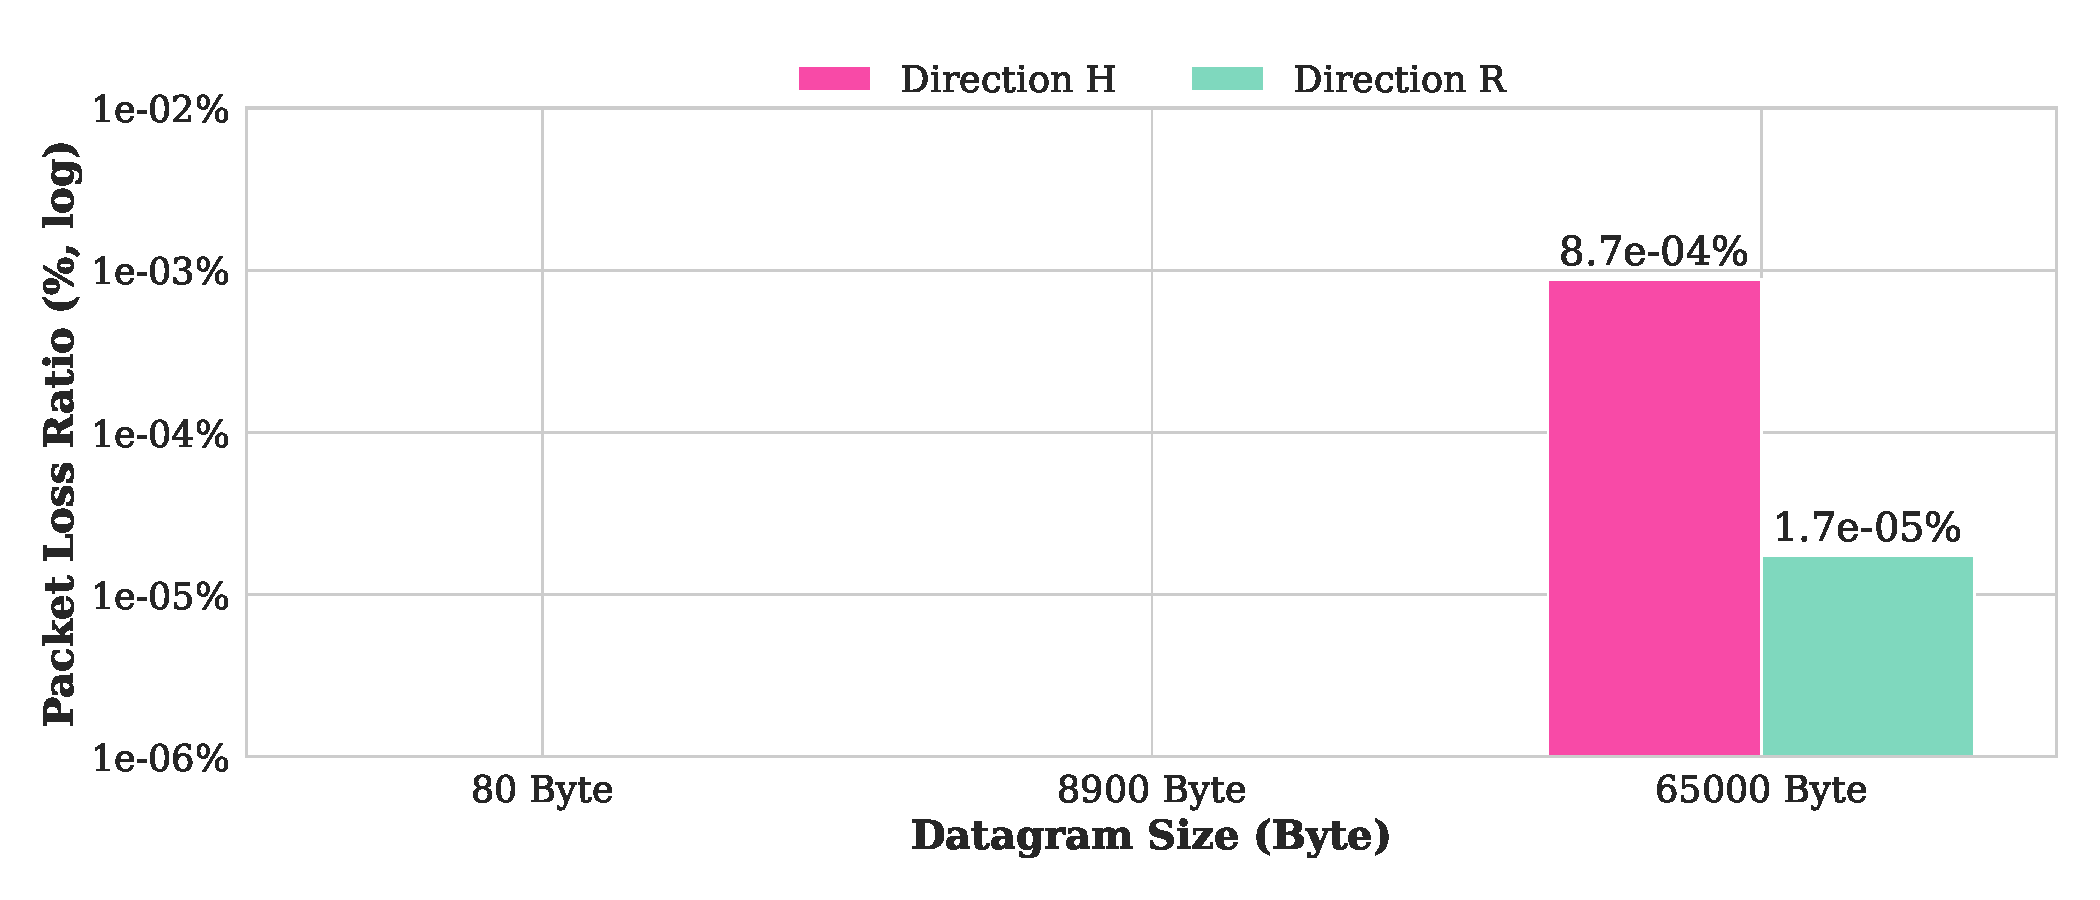
\includegraphics[width=1\linewidth]{figures/reliability/ihawk/diagr8.pdf}
    \caption{Packet Loss Ratio by Datagram Size and Communication Direction (Campaign `Tests with additional Load at the Center').}
    \label{fig:diagr8Loss}
\end{figure}

Figure \ref{fig:diagr8Loss} displays the results of the test campaign categorized by communication direction and datagram size. The results are consistent with those observed in the first test campaign (Figure \ref{fig:diagr3Loss}), as packet losses only occurred with a datagram size of 65000 bytes in both communication directions.

Packet losses were observed in the direction `H' (Center to Endpoints), which again only occurred during communication with endpoint 3. The reasons for those losses were already described in the previous section.

In direction `R' (Endpoints to Center), packet losses were also comparable to the results of the campaign without additional load. The loss ratio is with \num{1.75e-5} \% slightly higher than on the scenario without additional load (\num{7.56e-6} \%). A possible explanation for this might be a variation in the exact number of packet losses, as well as the shorter duration choosen for this campaign. The absolute number of these losses, however, is very low at 8 packets across all links in direction `R'.

\paragraph{Classification of Results}
The results of this campaign showed that the additional load on the iHawk in the center of the star had no impact on reliability, as the number of packet losses was comparable to the campaign with no additional load.


\subsubsection{Tests to Investigate the Influence of CPU Affinity} \label{chap:AffinityAnalysis}
\paragraph{Motivation and Context}

CPU affinity refers to the ability to bind processes to one or more specific CPU cores \cite{reli06}. The objective of this campaign is to examine the impact of various CPU affinity options applied to the center PC on the reliability.

As mentioned in \ref{chap:iHawkChar}, the iHawk's PCIe slots are directly connected to one of the CPUs. CPU 0 is connected to slots 1 to 3, which contain network cards connected to endpoints 2 and 3. Similarly, CPU 1 is connected to slots 4 to 6, which contain network cards connected to endpoints 1 and 4. The CPUs are interconnected through two UPI links. The purpose of the test campaign is to investigate any possible limitations in this two-socket configuration. These limitations could be caused by bottlenecks in the memory connection of the network cards and the connection between the CPUs.

If CPU affinity is not explicitly configured, the scheduler will assign arbitrary CPU cores to the corresponding TestSuite processes, as it has no information about which I/O devices are used by which process \cite{reli07}. In this test campaign, a scenario with 'enabled' CPU affinity was performed. This describes the situation when client and server processes of TestSuite were bound to the CPU cores on the local NUMA node. This refers to the CPU node to which the respective network card is connected. Additionally, a test was conducted usi`H'ng an 'inverse' CPU affinity, in which the processes of the TestSuite were configured to use CPU cores from the other socket. The Receive Side Scaling settings (see \ref{chap:ReceiveSideScaling}) of the network interface were not changed in all tests, as they are set by default to use only the cores on the local NUMA node.

Tests were performed with a duration of 10 minutes, using the same datagram sizes and a cycle time of 0 µs as in the previous campaigns.

\paragraph{Results}

\begin{figure}[h]
    \centering
    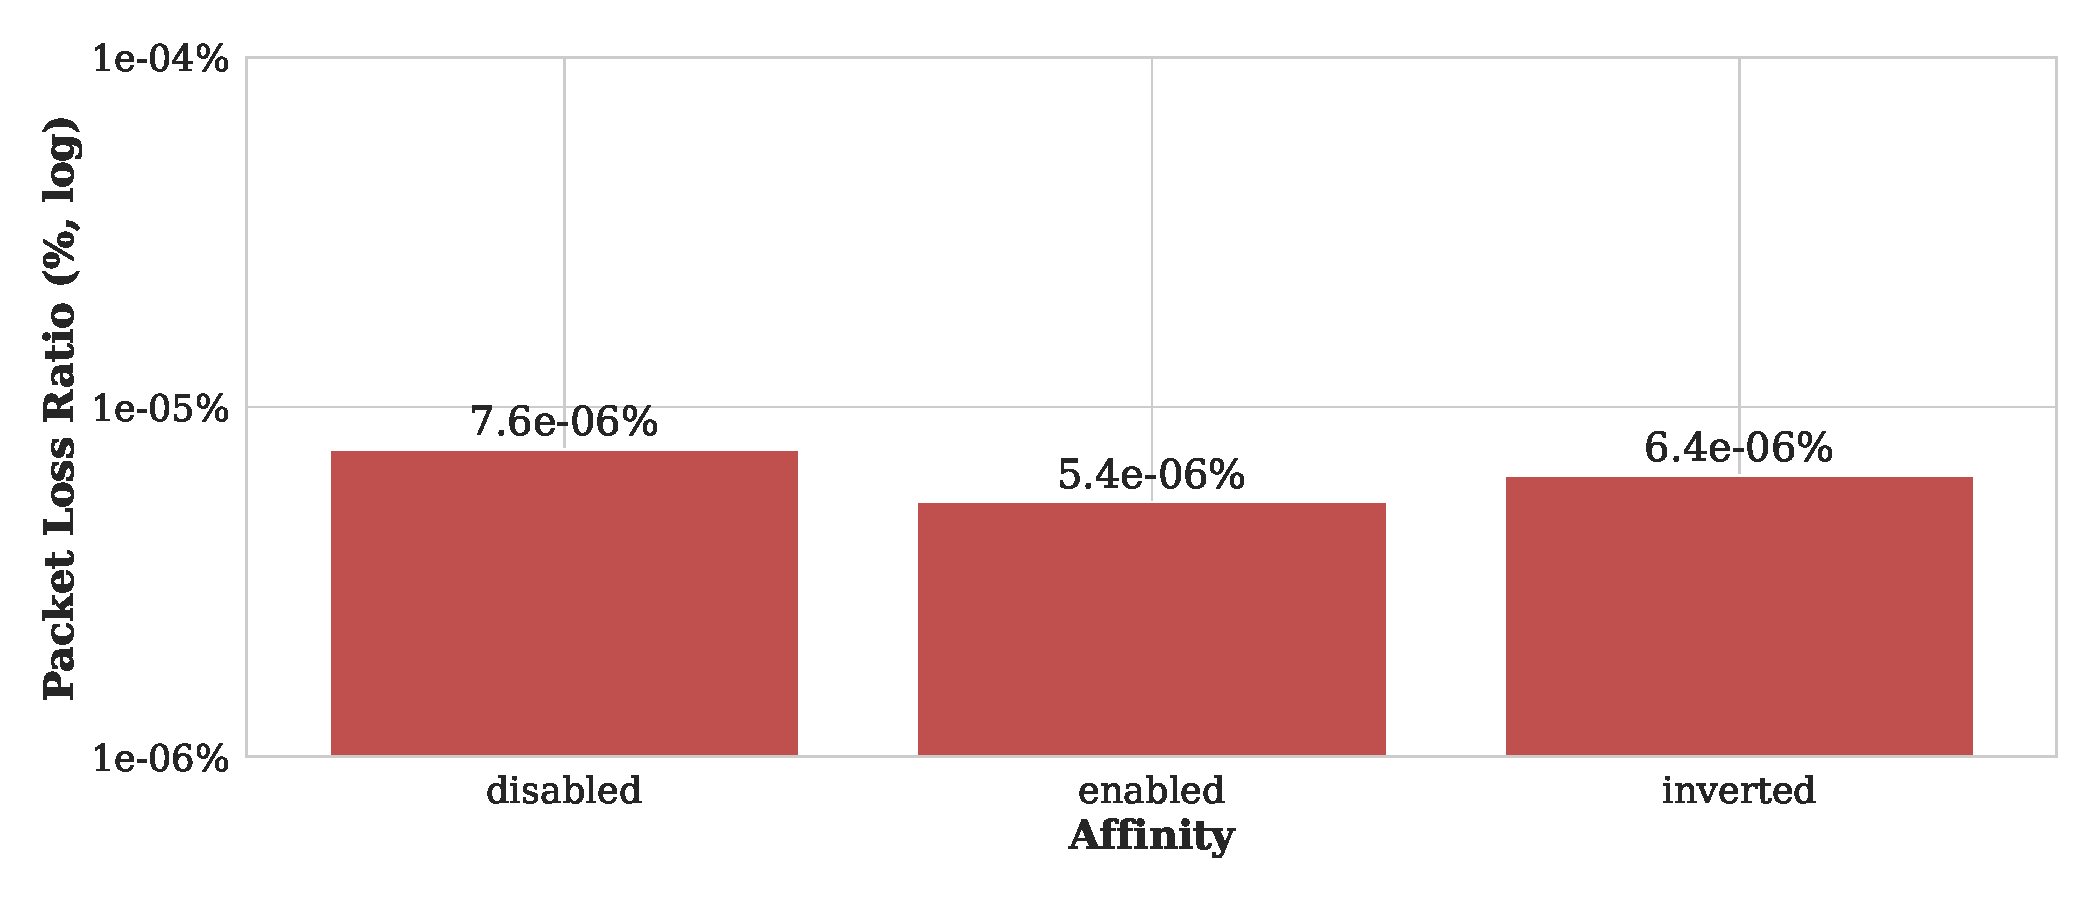
\includegraphics[width=1\linewidth]{figures/reliability/ihawk/diagr9.pdf}
    \caption{Packet Loss Ratio by Affinity Setting for a Datagram Size of 65000 Byte (Campaign `Tests to Investigate the Influence of CPU Affinity').}
    \label{fig:diagr9Loss}
\end{figure}

Figure \ref{fig:diagr9Loss} shows the packet losses using the two CPU affinity settings in the `R' direction (Endpoints to Center) for a datagram size of 65000 byte and compares them to the results with no affinity setting from a previous campaign. For all tests performed, packet losses were only detected with a datagram size of 65000 byte. The packet losses in the direction `H' (Center to Endpoints) will not be discussed in detail here, as no particular anomalies were observed compared to the other test campaigns. There were packet losses in the communication channels from the center to endpoint 3.

Packet losses were observed with all three affinity settings in direction `R' when the datagram size was 65000 bytes, which is in connection with fragmented packets. These losses were also observed in the previous test campaigns.  The packet loss ratio varies slightly depending on the affinity settings utilized, but remains within a comparable range, ranging from \num{7.6e-6} \%  to \num{5.4e-6} \%. These variations in individual tests result more from variations in the specific number of packet losses, combined with the relatively short duration of the tests, than from the different evaluated CPU affinity settings. The CPU utilization of the center is similar for all three CPU affinity choices being evaluated and have already been discussed in the 'Tests without additional Load' campaign (see \ref{chap:noaddloadTest}).

\begin{figure}[h]
    \centering
    \begin{subfigure}[b]{0.32\textwidth}
        \centering
        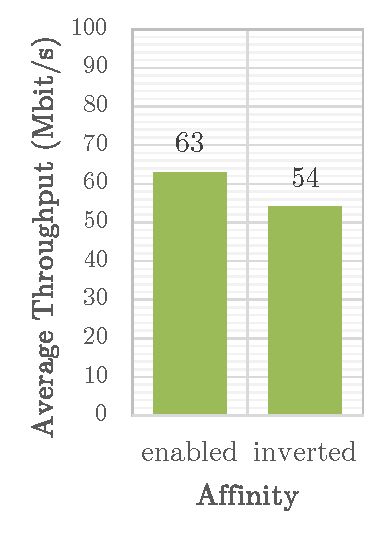
\includegraphics[width=\textwidth]{figures/reliability/ihawk/diagr10a.pdf}
        \caption{80 Byte}
    \end{subfigure}
    \hfill
    \begin{subfigure}[b]{0.32\textwidth}
        \centering
        \includegraphics[width=\textwidth]{figures/reliability/ihawk/diagr10b.pdf}
        \caption{8900 Byte}
    \end{subfigure}
    \hfill
    \begin{subfigure}[b]{0.32\textwidth}
        \centering
        \includegraphics[width=\textwidth]{figures/reliability/ihawk/diagr10c.pdf}
        \caption{65000 Byte}
    \end{subfigure}
    \caption{Average Throughput for different Affinity Settings (Campaign `Tests to Investigate the Influence of CPU Affinity').}
    \label{fig:diagr10Throuhput}
\end{figure}

One notable result of this test campaign is the difference in the average transmit throughput of the center. Figure \ref{fig:diagr10Throuhput} compares the transmit data rates between 'enabled' and 'inverted' CPU affinity. The results show that, for datagram sizes of 80 bytes and 8900 bytes, the send throughput is approximately 15\% higher for the 'enabled' CPU affinity scenario than for the 'inverted' CPU affinity test. For a datagram size of 6500 bytes, the send throughput is approximately 3\% higher. The higher throughput is due to the fact that the CPU can access its local resources much faster than the other CPU. The UPI Link, which connects the two CPU sockets, has a latency of about 130 ns \cite{setup07}.

\paragraph{Classification of Results}
The results of this test campaign indicate that CPU affinity does not affect system reliability. Furthermore, it is important to note that potential bottlenecks in multi-socket systems, do not have an impact on the packet loss rate of a UDP communication.


\subsubsection{Tests to Investigate the Influence of Interrupt-Moderation} \label{chap:RelInterMod}
\paragraph{Motivation and Context}

Interrupt moderation, described in \ref{chap:InterMod}, can reduce the number of interrupts generated by the network interface.

This campaign investigates the influence of different settings for interrupt moderation on reliability. The reliability will be examined with deactivated interrupt moderation, as used in all previous campaigns. The recommended timeout values of 84 µs (equivaltent to \num{\sim{12000}} interrupts/s) and 62 µs (equivaltent to \num{\sim{16000}} interrupts/s) from the Intel Linux Performance Tuning Guide \cite{intermod03} were also tested. Additionally, adaptive interrupt moderation, which is active by default, was examined.  

The test campaign included tests with three datagram sizes of 80, 8900, and 65000 bytes, each with a duration of 5 minutes.

\paragraph{Results}
No significant differences in reliability were found among the various rates of interrupt moderation and the scenario without such moderation. Similar to the test scenario with interrupt moderation disabled, low levels of packet loss in direction `R' were detected in all three variants tested. Furthermore, packet losses were also detected at endpoint 3, as discussed in previous sections.

\begin{figure}[h]
    \centering
    \includegraphics[width=1\linewidth]{figures/reliability/ihawk/diagr11.pdf}
    \caption{CPU Utilization in the Center for different Interrupt Moderation Configurations (Campaign `Tests to Investigate the Influence of Interrupt-Moderation').}
    \label{fig:diagr11CPU}
\end{figure}

Figure \ref{fig:diagr11CPU} displays CPU usage in the center with various interrupt moderation settings. As expected, the CPU usage reaches its maximum at about 54\% when interrupt moderation is disabled. All three datagram sizes exhibit similar values in this case. The two interrupt moderation rates of 84 µs and 62 µs record equally high CPU utilization rates of around 33\%, with slightly higher values observed for 62 µs. However, these two test scenarios revealed significant differences in datagram sizes across the various areas. When dealing with small datagrams, especially those of 80 byte in the test, a lower CPU utilization can be experienced. This is because a higher number of UDP packets per second are sent or received (\num{\sim{99000}} pps) compared to the other two datagram sizes (\num{\sim{81000}} pps for 8900 bytes and \num{\sim{19000}} pps for 65000 bytes). The utilization of interrupt moderation leads to a decrease in the number of interruptions generated and a reduction in CPU load.

Adaptive interrupt moderation demonstrated variations in CPU utilization between the examined datagram sizes when compared to a fixed moderation rate. In this case, the interrupt rate is adjusted to provide low latency or high throughput depending on the type of traffic. This process is explained in detail in the patent \cite{intermod04}. For small datagrams, a low interrupt moderation rate is selected, which is equivalent to a high number of interrupts per second. Conversely, for large datagrams, a high interrupt moderation rate is selected, which is equivalent to a lower number of interrupts per second. These results are consistent with the CPU usage, which is significantly higher for 80 bytes than for 8900 or 65000 bytes.

\paragraph{Classification of Results}
The campaign has shown that all examined interruption moderation rates exhibit comparable reliability. The differences in CPU utilization was also investigated.

Although adaptive interrupt moderation was found to be as reliable as other settings, it should not be used in the Distributed Test Support System at this time due to the uncontrollability of its implementation. While the function is described in \cite{intermod04}, the behavior of the implementation may be unpredictable if used without closer examination.

However, the interrupt moderation in connection with the selected interrupt rate also has an influence on the latency, which is considered in section 5. %TODO - Change Reference

\subsubsection{Tests with the Intel X540-T2 Network Interfaces in the Center} \label{chap:IntelRel540}
\paragraph{Motivation and Context}
This campaign investigates the reliability of the Intel X540-T2 network interface in the iHawk in the center of the star and compares it to the Intel X710-T2L network interface examined so far. Both interfaces are presented in \ref{chap:NicTypes} and have two RJ45 ports and are both 10 GbE capable. The X540 chipset network cards were released in 2012, which means they are 7 years older than the X710 chipset network cards, which were released in 2019 \cite{setupnw02, setupnw03}. In addition, interfaces use different drivers (see Table \ref{tab:drivernic}). Both devices offer comparable offloading mechanisms.

During testing, datagram sizes of 80 bytes, 8900 bytes, and 6500 bytes were considered with a cycle time of 0 µs and a test duration of 2 hours each.

\paragraph{Results}
The reliability results show no noticeable differences compared to the Intel X710-T2L network cards. In direction `R', a minimal number of packet losses were observed that can be attributed to the center, as previously mentioned. However, no packet losses were recorded in direction `H' during the test.

Moreover, there were no notable variations in the transmission data rates of the center achieved through the utilization of Intel X540-T2 network cards and those of Intel X710- T2L network cards. Both cards also show a similarly CPU utilization.

\paragraph{Classification of Results}
The results indicate that both network interfaces, the Intel X710-T2L and the Intel X540-T2, are suitable for use in the Distributed Test Support System from a reliability standpoint. 

\subsection{Insights}
Overall, packet losses were detected during the tests, but only under maximum load and in relation to fragmented packets with a size of 65,000 bytes. Therefore, although packet losses occurred, the investigated topology can still be considered suitable for a Distributed Test Support System.

No degradation was found with increased stress at the center or when changing the location of the CPU socket on which the send or receive process is executed. Additionally, no differences in reliability were found among the different interrupt moderation rates tested, despite a noticeable variation in CPU utilization.

The reliability of the Intel X540-T2 network card in the center was tested and no differences were found compared to the X710-T2L. Therefore, the Intel X540-T2 is also suitable for use in the center of a Distributed Test Support System.









	\chapter{Analysis of Performance} \label{chap:perfAnalysis}
The test campaigns presented here aim to investigate the performance of UDP communication in a local network under conditions similar to those in a Distributed Test Support System. The considered performance indicators are latency and jitter. The investigations are performed using the star topology with the iHawk in the center, presented in \ref{chap:TopoiHawk}.

Contrary to the investigation of reliability, no direct requirement can be defined here under which this test can be considered a success. The aim of the investigation is rather to determine the expected latencies, which may lead to certain restrictions concerning the use of a UDP communication within a Distributed Test Support System.

There are several factors that can contribute to the latency of a network. However, since there are no intermediate stations between the computer systems in the network topology, the focus will be on these computer systems and their operating states. In a computer system, latency is influenced by the network interface and driver, processing in the network stack, and the application. Prytz and Johannessen contend in \cite{perfnew01} that the latency is primarily determined by the performance of the end node.

The worst-case latency (see \ref{chap:LatencyExplanation}) is the most important indicator for these investigations. However, the mean latency should be also considered. Additionally, secondary data, such as packet losses and datagram sequence, are taken into consideration.

\section{System under Test}
Although the topology with the iHawk in the center is used, in contrast to the reliability tests with this topology (see \ref{chap:ReliabIhawk}), not all bi-directional links between the iHawk in the center and the High-Performance or Traffic PCs are to be examined simultaneously. Instead, a single isolated communication is considered.

\begin{figure}[h]
    \centering
    \begin{subfigure}[b]{0.48\textwidth}
        \centering
        \includegraphics[width=\textwidth]{figures/performance/sut_1a.pdf}
        \caption{Direction `H'}
        \label{fig:SutHpcPerf:H}
    \end{subfigure}
    \hfill
    \begin{subfigure}[b]{0.48\textwidth}
        \centering
        \includegraphics[width=\textwidth]{figures/performance/sut_1b.pdf}
        \caption{Direction `R'}
        \label{fig:SutHpcPerf:R}
    \end{subfigure}
    \caption{Illustration of the used System under Test with a High-Performance PC.}
    \label{fig:SutHpcPerf}
\end{figure}

The system under test is defined as the UDP communication generated by the TestSuite. Figure  \ref{fig:SutHpcPerf} illustrates this communication between the iHawk and HPC1. Both directions are considered in the campaigns. Direction '\textbf{H}', as depicted in Figure \ref{fig:SutHpcPerf:H}, refers to the communication with iHawk as the sender and HPC1 as the receiver. In contrast, Figure \ref{fig:SutHpcPerf:R} illustrates Direction '\textbf{R}', where HPC1 acts as the sender and iHawk as the receiver.

Similarly, a UDP communication between the iHawk and TPC1 was also considered a system under test. Again, both directions were analyzed.

The network interfaces mentioned in the topology description are used unless otherwise stated in the test campaign description. Furthermore, as with the reliability tests with the iHawk in the center, several settings recommended in the Intel Linux Performance Tuning Guide for the Ethernet 700 series were used. A list of these settings can be found in chapter \ref{chap:ReliabIhawk:SuT}.

\section{Accuracy of Measurements}
As showed in \ref{chap:LatencyExplanation}, latency calculation is based on the difference between two time stamps. One of them is recorded at the sender and the other at the receiver. In order to calculate a valid latency value, clock synchronization between the systems is required. The accuracy and reliability of the measurements depend on the accuracy of this clock synchronization.

As previously stated in \ref{chap:targetcom:timestamps}, PTP is utilized to synchronize clocks between systems. To minimize the interference between test execution and clock synchronization, a separate network with an Ethernet switch was used soley for clock synchronization, independent of the topology under investigation. This approach also reduces the configuration effort required for PTP.

The programs ptp4l and phc2sys implement the PTP standard for Linux. They provide information about the accuracy of the synchronization with the master offset \cite{perf02}. Table \ref{tab:PTPMasterOffset} shows this information for the setup used in the test. HPC1 was the master and TPC1 and the iHawk were the slaves.

\begin{table}[h]
\centering
\begin{tabular}{l|l|l}
	\toprule
	\textbf{System} & \textbf{Role} & \textbf{Master Offset} \\
	\midrule
 	HPC1 & Master & - \\ 
 	TPC1 & Slave & ±80 ns \\
 	iHawk & Slave & ±85 ns \\
	\bottomrule
\end{tabular}
\caption{PTP Master Offset in the Test Setup.}
\label{tab:PTPMasterOffset}
\end{table}

The data indicates that the clocks of the two slaves synchronize with the master with an accuracy of 80 to 85 ns. Since the measured latencies in the test are expected to be at least in the two- to three-digit microsecond range, the accuracy of the clock synchronization is sufficient to provide reliable latency results.

\clearpage
\section{Test Campaigns}
The first test campaign performed as part of the latency investigation is to examine the latency when using a High-Performance PC. The campaign includes a comparison of UDP sockets with Raw and Packet sockets. Subsequently, a campaign was conducted to investigate latency when using a Traffic PC. Additional campaigns were carried out to examine the influence of additional load, CPU affinity, and interrupt moderation. Finally, the latency when using Intel X540-T2 network interfaces was also investigated.

\subsection{Tests with UDP, Raw and Packet Sockets using a High-Performance PC} \label{chap:PerfSockType}
The purpose of this test campaign is to examine and compare the latency of UDP, Raw, and Packet sockets. Both the sender and receiver will use the respective socket type. No additional system load will be applied to either computer system.

\subsubsection{Test Setup}
The test campaigns will be carried out with datagram sizes ranging from 80 to 8080 bytes, increasing in steps of 1000 bytes. Additionally, a datagram size of 65000 bytes was tested for UDP sockets utilizing fragmentation.

All tests were conducted using the iHawk and HPC1 systems under test, with a cycle time of 0 µs used, which corresponds to an uninterrupted transmission process. The test duration for each datagram size was 60 seconds.

\subsubsection{Results}
\paragraph{Worst-Case Latency}

\begin{figure}[h!]
  \centering
  \subcaptionbox{Direction `H'\label{fig:SockTypeWc:a}}{%
    \includegraphics[width=1\textwidth]{figures/performance/d_2a.pdf}
  }
  \subcaptionbox{Direction `R'\label{fig:SockTypeWc:b}}{%
    \includegraphics[width=1\textwidth]{figures/performance/d_2b.pdf}
  }
  \caption{Worst-Case Latency by Datagram Size and Socket Type (Campaign `Tests with UDP, Raw and Packet Sockets using a High-Performance PC').}
  \label{fig:SockTypeWc}
\end{figure}

Figure \ref{fig:SockTypeWc} displays the worst-case latency for the three investigated socket types in relation to the datagram size. A distinction is made between direction `H' and `R'.

The worst-case latency for UDP sockets in direction `H' is 163.97 µs, while Raw sockets have a slightly higher worst-case latency of 169.32 µs. Packet sockets, on the other hand, have a slightly lower worst-case latency of 150.61 µs. Figure \ref{fig:SockTypeWc:a} illustrates the worst-case latency as in relation of datagram size. The figure shows that the worst-case latency fluctuates, but no trend is apparent from the data.

The worst-case latency in direction `R' is significantly lower than in direction `H'. When using UDP sockets, the worst-case latency is 109.31 µs, with Raw sockets it is 81.19 µs, and with Packet sockets it is 93.87 µs. Figure \ref{fig:SockTypeWc:b} displays the worst-case latency as a function of datagram size, but again no trend can be identified.

It is noticeable that the measured worst-case latency in the `R' direction is 33\% lower than in direction `H' when using UDP sockets. This reduction is even greater at 52\% when using Raw sockets. The exact reason for this difference is difficult to determine at this point due to the inability to obtain time stamps from the network interface, which makes it impossible to identify which system causes how much latency. Both systems use the same network interface, so a likely cause of these differences between directions `H' and `R' is the different hardware of the systems. As \cite{perfnew01} suggests, latency is primarily determined by the performance of the end node. Since the iHawk as receiver in direction 'R' has a more powerful hardware, this could be a reason for the observed lower latencies in this direction.

When examining the time distribution of latencies, it is evident that the highest latencies (worst-case latencies) consistently occur for the first 10 packets sent during the test. This applies to all socket types in both directions. As previously mentioned, no time stamps can be obtained from the network interface, making it difficult to analyze the reason for this observation.

During the tests, no packet losses were detected with any of the three socket types examined. However, it was found that when Packet sockets are used in both directions `H' and `R', the packets are re-sorted and do not arrive in the correct order. This behavior was not observed with UDP sockets and Raw sockets.

\paragraph{Mean Latency}

Figure \ref{fig:SockTypeMl} shows the mean latency for different datagram sizes, compared across the three examined socket types.

\begin{figure}[h!]
  \centering
  \subcaptionbox{Direction `H'\label{fig:SockTypeMl:a}}{%
    \includegraphics[width=1\textwidth]{figures/performance/d_3a.pdf}
  }
  \subcaptionbox{Direction `R'\label{fig:SockTypeMl:b}}{%
    \includegraphics[width=1\textwidth]{figures/performance/d_3b.pdf}
  }
  \caption{Mean Latency by Datagram Size and Socket Type (Campaign `Tests with UDP, Raw and Packet Sockets using a High-Performance PC').}
  \label{fig:SockTypeMl}
\end{figure}

In the direction `H', the mean latency is 26.4 µs across all datagram sizes when using UDP sockets. Raw socket have has a comparable mean latency of 27.15 µs. Packet sockets had the lowest mean latency of 21.83 µs, which is 17\% lower than UDP sockets.

Figure \ref{fig:SockTypeMl:a} illustrates the correlation between datagram size and mean latency. The data indicates that as the size of the datagram increases, the mean latency also increases. This is primarily due to the fact that larger packets require more processing.

In the direction `R', UDP sockets had a mean latency of 24.67 µs. Raw sockets and Packet sockets had a mean latency that was approximately 10\% lower, as shown in Figure \ref{fig:SockTypeMl:b}. The figure also demonstrates that the mean latency increases also in this direction when the datagram size is increased. The mean latency in direction `R' is lower than that in direction `H'.

\paragraph{Influence of Fragmentation on Latency}

The campaign also examined the latency associated with fragmentation, using a datagram size of 65000 bytes as an example. The test was only performed with UDP sockets, as Raw and Packet sockets do not support fragmentation.

\begin{figure}[h!]
  \centering

  \begin{subfigure}[b]{0.45\linewidth}
    \includegraphics[width=\linewidth]{figures/performance/d_4a.pdf}
    \caption{80 Byte}
    \label{fig:histFrag:a}
  \end{subfigure}
  \hfill
  \begin{subfigure}[b]{0.45\linewidth}
    \includegraphics[width=\linewidth]{figures/performance/d_4b.pdf}
    \caption{8900 Byte}
    \label{fig:histFrag:b}
  \end{subfigure}

  \begin{subfigure}[b]{0.45\linewidth}
    \includegraphics[width=\linewidth]{figures/performance/d_4c.pdf}
    \caption{65000 Byte}
    \label{fig:histFrag:c}
  \end{subfigure}
  \hfill
  \begin{subfigure}[b]{0.45\linewidth}
    \includegraphics[width=\linewidth]{figures/performance/d_4d.pdf}
    \caption{65000 Byte (enlarged Section)}
    \label{fig:histFrag:d}
  \end{subfigure}
  
  \caption{Latency Distribution for UDP Sockets with different Datagram Sizes in Direction `H' (Campaign `Tests with UDP, Raw and Packet Sockets using a High-Performance PC').}
  \label{fig:histFrag}
\end{figure}

Figure \ref{fig:histFrag} displays histograms of the latency for datagram sizes of 80 bytes, 8900 bytes and 65000 bytes in direction `H'. Figure \ref{fig:histFrag:d} presents an enlarged version of the histogram, showing only the section from 150 µs to 300 µs.

With a datagram size of 65000 bytes (see Figure \ref{fig:histFrag:c}), a worst case latency of 3431.16 µs was observed, which is more than 20 times higher than with a datagram size of 8900 bytes (163.97 µs). The mean latency for a datagram size of 65000 bytes is 215.78 µs, which is approximately 7.5 times higher than for a datagram size of 8900 bytes. This difference can be attributed to fragmentation (see \ref{chap:frag}). When a UDP datagram with a size of 65000 bytes is sent, it is divided into 8 packets at an MTU of 9000 bytes. This correlates with the observed increase in mean latency.

While the distribution is close to the mean for datagram sizes of 80 bytes (see Figure \ref{fig:histFrag:a}) and 8900 bytes (see Figure \ref{fig:histFrag:b}), indicating low Jitter. However, for a datagram size of 65000 bytes, a wider distribution can be seen. Upon closer inspection of the enlarged section in Figure \ref{fig:histFrag:d}, a multimodal distribution is observed.

Additionally, it was discovered that datagrams are rearranged at a datagram size of 65000 bytes due to fragmentation.  These fundamental observations about fragmentation also apply to direction `R'.

\subsubsection{Classification of Results}
One outcome of this campaign is that Packet have a lower worst-case and mean latency than UDP sockets or Raw sockets, but it was observed as a secondary result observed that packets do not arrive in the application in the order in which they were sent. Another argument against Packet sockets is that they are more complex to handle, since layer 2, 3, and 4 headers must be generated by the application. For this reason, this Socket Type will not be considered in the further performance analysis.

The campaign also revealed that Raw sockets have a latency comparable to that of UDP sockets. However, they are also more complex to handle than UDP sockets, so they are not considered in the following campaigns.

Regarding fragmentation, the campaign discovered that latency increases significantly for datagram sizes above the MTU due to fragmentation. Additionally, it was observed that fragmented packets arrive in reverse order.


\subsection{Tests with UDP Sockets using a Traffic PC}
The purpose of this test campaign is to examine the latency of the system under test utilizing the iHawk and a Traffic PC. Both directions `H' and `R' are considered.

\subsubsection{Test Setup}
Based on the results of the previous test campaign 'Tests with UDP, Raw and Packet Sockets' (see \ref{chap:PerfSockType}), the tests were performed only with UDP sockets and datagram sizes from 80 to 8080 bytes in steps of 1000 bytes. The cycle time and test duration used in this campaign are the same as in the previous one.

\subsubsection{Results}
\paragraph{Worst-Case Latency}

\begin{figure}[h!]
  \centering
  \subcaptionbox{Direction `H'\label{fig:TrafficWc:a}}{%
    \includegraphics[width=1\textwidth]{figures/performance/d_5a.pdf}
  }
  \subcaptionbox{Direction `R'\label{fig:TrafficWc:b}}{%
    \includegraphics[width=1\textwidth]{figures/performance/d_5b.pdf}
  }
  \caption{Worst-Case Latency by Datagram Size and System under Test (Campaign `Tests with UDP Sockets using a Traffic PC').}
  \label{fig:TrafficWc}
\end{figure}

Figure \ref{fig:TrafficWc} displays the worst-case latency for the system under test with a Traffic PC. Additionally, the results from the previous test campaign (see \ref{chap:PerfSockType}) for a UDP socket with a high performance PC as the system under test are shown for comparison.

In direction `H' a worst case latency of 229.20 µs was measured. Figure \ref{fig:TrafficWc:a} shows it in relation to the datagram size. The worst-case latency of the system under test with a Traffic PC is therefore approximately 30\% higher than with a High Performance PC.

Possible reasons for the higher latency in the direction `H' compared to a High-Performance PC are the  less capable hardware of the Traffic PCs, resulting in a longer processing time of a received packet in the network stack. Additionally, the Traffic PCs use different network cards that use a different driver.

In the `R' direction, the worst-case latency is 80.73 µs, which is 26\% lower than the worst-case latency of a High-Performance PC used as the system under test. This could be due to the use of a different network interface, the Intel X540-T2, in the Traffic PCs.

\paragraph{Mean Latency}
\begin{figure}[h!]
  \centering
  \subcaptionbox{Direction `H'\label{fig:TrafficMean:a}}{%
    \includegraphics[width=1\textwidth]{figures/performance/d_6a.pdf}
  }
  \subcaptionbox{Direction `R'\label{fig:TrafficMean:b}}{%
    \includegraphics[width=1\textwidth]{figures/performance/d_6b.pdf}
  }
  \caption{Mean Latency by Datagram Size and System under Test (Campaign `Tests with UDP Sockets using a Traffic PC').}
  \label{fig:TrafficMean}
\end{figure}

Regarding the mean latency in Direction `H' with a traffic PC in the system under test, shown in Figure \ref{fig:TrafficMean:a}, it can be observed that it is 108.79 µs on average. This is 76\% higher than in the tests with a High-Performance PC. In direction `R', shown in figure \ref{fig:TrafficMean:b}, the average mean latency is 24.8 µs, which is almost the same as the average latency measured in the tests with a High-Performance PC. In both directions, there is an increase in latency as the datagram size increases.

\subsubsection{Classification of Results}
The test campaign examined the latency of UDP communication with a Traffic PC in the setup and compared it to a setup with a High-Performance PC.

It was found that the latency in direction "H" is higher for communication between the iHawk and a Traffic PC than for communication between the iHawk and a High-Performance PC. This applies to both the worst-case and mean latency. In contrast, in the `R' direction, a significantly lower worst-case latency and a comparably high average latency are observed.


\subsection{Tests with additional Load using a High-Performance PC}
The purpose of this test campaign is to analyze and compare latency under different load situations.

One load situation is to stress all participating computer systems. For this purpose, the realistic load scenario described in Table \ref{tab:realpc} is used. The number and intensity of the stress-ng stressors remain the same. However, no network stressors are used as the focus of this load scenario is on the computer systems.

Additionally, the overall system is subjected to network load. The TestSuite is used to generate a maximum network load through UDP communications with a datagram size of 8900 bytes and a maximum bandwidth of 10 GBit/s between the iHawk in the center and all participating computer systems of the topology used, resulting in 7 generated bidirectional communications. This is comparable to the load in the reliability test with the iHawk in the center (refer to Figure \ref{fig:topoihawknaming}). No additional network load is generated on communication link 1A, where the latency is measured.

\subsubsection{Test Setup}
The tests were conducted using UDP sockets and datagram sizes ranging from 80 to 8080 bytes in increments of 1000 bytes. A cycle time of 0 µs and a test duration of 60 seconds were utilized. Only the system under test with the High-Performance PC was evaluated.

\subsubsection{Results}
\paragraph{Worst-Case Latency}

\begin{figure}[h!]
  \centering
  \subcaptionbox{Direction `H'\label{fig:StressWc:a}}{%
    \includegraphics[width=1\textwidth]{figures/performance/d_7a.pdf}
  }
  \subcaptionbox{Direction `R'\label{fig:StressWc:b}}{%
    \includegraphics[width=1\textwidth]{figures/performance/d_7b.pdf}
  }
  \caption{Worst-Case Latency by Datagram Size and Load Scenario with the System under Test with a High-Performance PC (Campaign `Tests with additional Load using a High-Performance PC').}
  \label{fig:StressWc}
\end{figure}

Figure \ref{fig:StressWc} displays the worst-case latency under additional system and network load in directions `H' and `R' and compares it to the worst-case latency without additional load.

The realistic scenario causes a CPU utilization of 19.5\% on the iHawk and 47.8\% on the High-Performance PC during the test. In both directions, the worst-case latency remains unaffected by the system load from the realistic scenario. The worst-case latency values are similar to those without additional load.

A network load in direction `H' (Center to Endpoint) also causes only a small increase in worst-case latency compared to the test with no additional load. The worst-case latency in this direction is 180 µs.

However, in direction `R' (Endpoint to Center), maximum network load causes a significant increase in worst-case latency, as shown in Figure \ref{fig:StressWc:b}. The maximum value, measured in tests with a datagram size of 7080 bytes, is 721.73 µs. Additionally, there is a more noticeable variation in worst-case latency across different datagram sizes. This increase is due to the high network load on the iHawk in the center. In addition to the measured communication, the system is stressed with 7 additional links of bidirectional communication, each with an average throughput of 9.68 GBit/s per direction. This high load is causing additional latency during processing in the receiving system.

\begin{figure}[h!]
    \centering
    \includegraphics[width=1\linewidth]{figures/performance/d_13.pdf}
    \caption{Worst-Case Latency by Datagram Size and Number of Links in Direction 'R' with the System under Test with a High-Performance PC (Campaign `Tests with additional Load using a High-Performance PC').}
    \label{fig:NetLoadLinkReduction}
\end{figure}

To examine the worst-case latency not only at the maximum network load of 7 bidirectional links, additional tests were performed. These tests analyzed latencies with different numbers of links that generate additional load. The results are presented in Figure \ref{fig:NetLoadLinkReduction}.

The results show that the highest worst case latency of 721.73 µs occurs when using 7 links. However, with 6 and 5 bidirectional links, the worst case latency is reduced to approximately 480 µs, a 33\% reduction compared to the use of 7 links. A further significant reduction to 175.84 µs is observed when using 4 links. When using 3, 2 or 1 bidirectional links, the worst-case latency is comparable to the latency no additional network load.

\paragraph{Mean Latency}
When both computer systems were stressed with the realistic load scenario, average latencies were observed in both directions that were comparable to the tests without load. This also applies to the network load in the direction `H'.

However, when maximum network load with 7 links was applied in the `R' direction, a significantly higher mean latency was observed compared to the test without additional load, as already described for the worst-case latency. The mean latency in this direction was 243.67 µs, which is almost 10 times higher than without additional load (24.67 µs). As the number of links decreases, the mean latency also decreases. Here too, no difference in mean latency was observed when using 3, 2, or 1 links compared to the tests without additional load.

\subsubsection{Classification of Results}
The results of the campaign suggest that the latency is not affected by additional system load, such as those from realistic scenarios, which involves CPU load, I/O load, and interrupt load.

When a network load is applied, the worst-case latency increased 4.5 times in direction `R', but remained unchanged in direction `H'. This is due to the high network load in the center. It is important to note that this scenario involved applying maximum utilization to all available communication channels.

\subsection{Tests to Investigate the Influence of CPU Affinity}
This campaign aims to investigate the impact of CPU affinity on latency. Such an investigation has already been done as part of the reliability analysis, so please refer to \ref{chap:AffinityAnalysis} for a detailed description of the goal and motivation of this campaign.

\subsubsection{Test Setup}
The tests in this campaign examine the CPU affinity option 'enabled' and compare it to no affinity setting. The tests are performed with UDP sockets and datagram sizes from 80 to 8080 bytes in steps of 1000 bytes. A cycle time of 0 µs and a test duration of 60 seconds were used. Only the system under test with the High-Performance PC was used.

\subsubsection{Results}
\paragraph{Worst-Case Latency}

\begin{figure}[h!]
  \centering
  \subcaptionbox{Direction `H'\label{fig:AffWc:a}}{%
    \includegraphics[width=1\textwidth]{figures/performance/d_8a.pdf}
  }
  \subcaptionbox{Direction `R'\label{fig:AffWc:b}}{%
    \includegraphics[width=1\textwidth]{figures/performance/d_8b.pdf}
  }
  \caption{Worst-Case Latency by Datagram Size and Affinity Setting with the System under Test with a High-Performance PC (Campaign `Tests to Investigate the Influence of CPU Affinity').}
  \label{fig:AffWc}
\end{figure}

Figure \ref{fig:AffWc} shows the worst-case latencies for the two investigated CPU affinity settings in both directions, `H' and `R'.

In direction `H' (Center to Endpoint), a maximum worst case latency of 144.76 µs was observed with CPU affinity enabled, which is 11.7\% lower than without CPU affinity enabled. In direction `R' (Endpoint to Center), a 12.4\% reduction in worst-case latency was observed. Again, as in the previous test campaigns, a higher latency was observed in direction `H' than in direction `R'.

It can be assumed that with configured CPU affinity, the fact that the CPU can access its local resources faster than the resources of the remote CPU has a positive influence on the worst-case latency. As explained in \ref{chap:iHawkChar}, accessing resources from the other CPU via the UPI link results in a latency of around 130 ns \cite{setup07}. This value is small compared to the measured latencies of UDP communication, which typically range from double to triple digits in microseconds. However, if CPU affinity is not taken into account, the latency caused by the UPI link can occur multiple times, resulting in a higher worst-case latency.

\paragraph{Mean Latency}

In both directions a mean latency comparable to the mean latency without CPU affinity could be observed for all datagram sizes with enabled CPU affinity (see Figure \ref{fig:SockTypeWc}, Data Series 'UDP Socket'). The maximum deviation observed was 1 µs.

\subsubsection{Classification of Results}
The campaign results indicate that enabling CPU affinity reduces worst-case latency by over 10\% compared to when CPU affinity is not enabled. CPU affinity has no effect on the mean latency.

\subsection{Tests to Investigate the Influence of Interrupt Moderation}
The purpose of this campaign is to analyze the latency associated with various interrupt moderation configurations.

Interrupt moderation, which can decrease the number of interrupts generated by the network interface, is described in \ref{chap:InterMod}. When examining reliability under different interrupt moderation settings (see \ref{chap:RelInterMod}), it was found that the options examined did not differ in the number of packet losses, but did vary in CPU utilization.

\subsubsection{Test Setup}
In addition to the previously used disabled interrupt moderation, the timeout values 62 µs and 84 µs recommended in the Intel Linux Performance Tuning Guide \cite{intermod03} as well as the adaptive interrupt moderation were examined. Tests were conducted using UDP sockets and datagram sizes ranging from 80 to 8080 bytes in increments of 1000 bytes. A cycle time of 0 µs and a test duration of 60 seconds were utilized. The campaign only considered the system under test with the High-Performance PC.

\subsubsection{Results}
\paragraph{Worst-Case Latency}

\begin{figure}[h!]
  \centering
  \subcaptionbox{Direction `H'\label{fig:IMWc:a}}{%
    \includegraphics[width=1\textwidth]{figures/performance/d_9a.pdf}
  }
  \subcaptionbox{Direction `R'\label{fig:IMWc:b}}{%
    \includegraphics[width=1\textwidth]{figures/performance/d_9b.pdf}
  }
  \caption{Worst-Case Latency by Datagram Size for different Interrupt Moderation Configurations with the System under Test with a High-Performance PC (Campaign `Tests to Investigate the Influence of Interrupt-Moderation').}
  \label{fig:IMWc}
\end{figure}

Figure \ref{fig:IMWc} displays the worst-case latency for various interrupt moderation configurations in direction `H' and `R'.

The highest worst-case latency in direction `H' is observed with interrupt moderation set to a timeout of 84 µs, with a maximum of 476.73 µs. The setting with a timeout value of 62 µs has a worst-case latency of 226.05 µs, which is considerably lower. With adaptive interrupt moderation, a worst case latency of 211.16 µs was observed with a datagram size of 3080 bytes. However, when interrupt moderation was disabled, the lowest worst-case latency was observed at 163.97 µs. Figure \ref{fig:IMWc:a} shows the worst-case latency against datagram size for all interrupt moderation configurations. No clear trend can be identified.

In direction `R', the highest worst-case latency of 488.94 µs is also observed with interrupt moderation set to a timeout value of 84 µs. Adaptive interrupt moderation has a worst-case latency of 214.11 µs in this direction, which is similar to the value in the `H' direction. With a timeout value of 62 µs, a worst-case latency of 158.13 µs is measured, while the lowest worst-case latency of 109.31 µs is also observed in this direction with disabled interrupt moderation. Similar to previous campaigns, the worst-case latency is lower in direction `R' compared to direction `H', except for adaptive interrupt moderation.

The finding that the timeout values have a higher worst-case latency than the disabled interrupt moderation was expected, since interrupt moderation, as described in \ref{chap:InterMod}, delays the generation of interrupts.  The worst-case latency in both directions for adaptive interrupt moderation ranges from 210 µs to 215 µs. Based on the test results, no clear dependency between datagram size and latency can be recognized for this configuration, although the description of the functionality (see \ref{chap:InterMod}) suggests otherwise.

\paragraph{Mean Latency}

Figure \ref{fig:IMean} shows the mean latency based on datagram size and interrupt moderation configuration.

The results show that activating interrupt moderation with a timeout value of 62 µs increases the average latency in direction `H' by more than two times and in direction `R' by more than three times. As expected, the configuration with a timeout value of 84 µs has an even higher mean latency.

The mean latency for adaptive interrupt moderation is 103 µs in both directions, making it the highest observed mean latency. Figure \ref{fig:IMean} shows a slight increase in mean latency with increasing datagram size. The interrupt moderation rate for adaptive interrupt moderation is determined by the number of connections and packet size. In this test with a low number of connections, a high number of interrupts per second should be configured for low latency \cite{intermod04}. However, this behavior cannot be confirmed in the performed tests, as the measured average latency is the highest compared to the other options examined. One possible reason for this could be the test duration, which may be too short for the adaptive interrupt moderation to configure itself.

\begin{figure}[h!]
  \centering
  \subcaptionbox{Direction `H'\label{fig:IMean:a}}{%
    \includegraphics[width=1\textwidth]{figures/performance/d_10a.pdf}
  }
  \subcaptionbox{Direction `R'\label{fig:IMean:b}}{%
    \includegraphics[width=1\textwidth]{figures/performance/d_10b.pdf}
  }
  \caption{Mean Latency by Datagram Size for different Interrupt Moderation Configurations with the System under Test with a High-Performance PC (Campaign `Tests to Investigate the Influence of Interrupt-Moderation').}
  \label{fig:IMean}
\end{figure}

\subsubsection{Classification of Results}
The results indicate that latency is at its lowest when interrupt moderation is deactivated. Additionally, the campaign presents the expected worst-case and mean latencies for interrupt moderation configurations with timeout values of 62 µs and 84 µs.

The highest latencies were measured with an adaptive interrupt configuration. However, the configuration changes due to factors such as the number of packets, packet size, or number of connections. As a result, the measured latency may fluctuate, making this option unsuitable for use in a Distributed Test Support System.

\subsection{Tests with the Intel X540-T2 Network Interface}
This campaign aims to investigate the latency of the Intel X540-T2 network interfaces in both iHawk and HPC1. The reliability of these interfaces has already been examined in \ref{chap:IntelRel540}, where no difference was found compared to the currently used Intel X710-T2L.

\subsubsection{Test Setup}
The test also employed the settings from the Intel Linux Performance Tuning Guide (see \cite{intermod03}) for the Intel X540-T2 network interfaces. This means for example that interrupt moderation is disabled.

The test mode used for this campaign was the same as in the previous campaigns. This involved the use of UDP sockets and datagram sizes ranging from 80 to 8080 bytes, with a cycle time of 0 µs and a test duration of 60 seconds. Only the system under test with the High-Performance PC was utilized.

\subsubsection{Results}
\paragraph{Worst-Case Latency}

Figure \ref{fig:540Wc} shows the worst-case latency when using the Intel X540-T2 network interfaces compared to the Intel X710-T2L network interfaces in both directions.

\begin{figure}[h!]
  \centering
  \subcaptionbox{Direction `H'\label{fig:540Wc:a}}{%
    \includegraphics[width=1\textwidth]{figures/performance/d_11a.pdf}
  }
  \vspace{10pt}
  \subcaptionbox{Direction `R'\label{fig:540Wc:b}}{%
    \includegraphics[width=1\textwidth]{figures/performance/d_11b.pdf}
  }
  \caption{Worst-Case Latency by Datagram Size of the Intel X540-T2 Network Interface compared with the Intel X710-T2L Network interface (Campaign `Tests with the Intel X540-T2 Network Interface').}
  \label{fig:540Wc}
\end{figure}

The results show that the worst-case latency is greater when using the Intel X540-T2 in both directions compared to the Intel X710-T2L. Across all datagram sizes, the worst-case latency is 257.79 µs in direction `H' and 229.56 µs in direction `R'.

The higher worst-case latencies with the same configuration with the Intel X540-T2 can be attributed to the fact that the network interface itself is older compared to the Intel X710-T2L. Additionally, the network interfaces use different drivers (see Table \ref{tab:drivernic}), which also affects the latency.

\paragraph{Mean Latency}

\begin{figure}[h!]
  \centering
  \subcaptionbox{Direction `H'\label{fig:540Mean:a}}{%
    \includegraphics[width=1\textwidth]{figures/performance/d_12a.pdf}
  }
  \subcaptionbox{Direction `R'\label{fig:540Mean:b}}{%
    \includegraphics[width=1\textwidth]{figures/performance/d_12b.pdf}
  }
  \caption{Mean Latency by Datagram Size of the Intel X540-T2 Network Interface compared with the Intel X710-T2L Network interface (Campaign `Tests with the Intel X540-T2 Network Interface').}
  \label{fig:540Mean}
\end{figure}


Figure \ref{fig:540Mean} displays a comparison of the mean latency of the Intel X540-T2 and Intel X710-T2L network interfaces. The mean latency in both directions, `H' and `R', increases with larger datagram sizes and is on average about 90.30 µs in direction `H' and 98.34 µs in direction `R'.

It is noticeable that with a datagram size of 80 bytes, the average latency in both directions has a value of about 42 µs and increases significantly with a datagram size of 1080 bytes. These differences are not observable when using the Intel X710-T2L network interfaces with small datagrams.

\subsubsection{Classification of Results}
The campaign has demonstrated that the Intel X540-T2 network interfaces exhibit significantly higher worst-case and mean latencies than the Intel X710-T2L network interfaces with the same configuration. Therefore, when using these network interfaces in the Distributed Test Support System, a higher latency should be expected. \\

\clearpage
\section{Insights} \label{insight:perf}
The test campaigns conducted to investigate the performance of an topology with an iHawk at the center provided the following key insights:

\begin{enumerate}[label=(\roman*),resume]
    \item The analysis revealed the anticipated latencies of a UDP communication on the application level. The lowest latencies are to be expected when communication is between the iHawk and a High-Performance PC. However, when communicating systems similar to Traffic PCs, higher latencies should be expected in some cases. \label{insight:perf:1}
    \item The analysis also examined latencies with Raw sockets and Packet sockets, in addition to UDP sockets. The results indicate that Packet sockets have lower latency than the other socket types, but sometimes packets do not arrive in the order in which they were sent. \label{insight:perf:2}
    \item Upon examination of the temporal distribution of latencies, it was found that the highest latencies occur during the first 10 transmitted packets. Therefore, it may be useful to integrate a warm-up phase in the Distributed Test Support System as part of the initialization process, during which a few packets are exchanged.
    \item Furthermore, the impact of different load scenarios on the participating computer systems was analyzed. The study found that exceptionally high network load on the receiving side using seven bidirectional links increases the worst-case latency by a factor of seven. However, when using three or fewer links to generate load, no increase in latency can be noticed. Similarly, a system with load comparable to the Test Support System shows no increase in latency. \label{insight:perf:3}
    \item The analyis investigated the impact of CPU affinity on multi-socket systems and found that it has a minor effect on latency. Also the latencies can be expected with different interrupt moderation options are presented. As expected, the lowest latency was observed when interrupt moderation was disabled. \label{insight:perf:4}
    \item Additionally, the investigation examined the latency of the Intel X540-T2 network interface and found it to be higher than that of the newer Intel X710-T2L network interface. \label{insight:perf:5}
    \item These observed latencies and their variation with respect to the computer system, network hardware, and system load must be taken into account when using a UDP-based implementation in a Distributed Test Support System. \label{insight:perf:6}
\end{enumerate}


 






	\textbf{NOCH NICHT IN DIESER VERSION:}
	\begin{itemize}
		\item Kapitel 1 – Einleitung
		\item Kapitel 6 – Conclusion, Zusammenfassung der Konfigurationen / Punkte woduch UDP geeignet ist
		\item Kapitel 7 – Ausblick: Fragmentierung und DPDK (User Space Driver)
		\item Anhang (mit Code)
	\end{itemize}
	
	
	\bibliography{bibliography/references.bib}
	\bibliographystyle{plainurl}
    
    
    \begin{appendix}
    	\chapter{Anhang}
Der Anhang kann Teile der Arbeit enthalten, die im Hauptteil zu weit führen würden, aber trotzdem für manche Leser interessant sein könnten. Das können z.\,B. die Ergebnisse weiterer Messungen sein, die im Hauptteil nicht betrachtet werden aber trotzdem durchgeführt wurden. Es ist ebenfalls möglich längere Codeabschnitte anzuhängen. Jedoch sollte der Anhang kein Ersatz für ein Repository sein und nicht einfach den gesamten Code enthalten.

		\listoffigures
		\listoftables
		\lstlistoflistings
    \end{appendix}
    
\end{document}
